\begin{savequote}[75mm]
Nature laughs at the difficulties of integration.
\qauthor{--- Pierre-Simon Laplace ---}
\end{savequote}


\chapter{Integration}
\label{chap_int}
\graphicspath{{figures/Int/}}

We have spent considerable time considering the derivatives of a function and their applications. In the following chapters, we are going to starting thinking in the other direction. That is, given a function $f(x)$, we are going to consider functions $F(x)$ such that $F'(x) = f(x)$. These functions will help us compute area, volume, mass, force, pressure, work, and much more.



\section{Antiderivatives and (in)definite integration}\label{sec:antider}
\subsection{Antiderivatives and indefinite integration}
Given a function $y=f(x)$, a \textbf{differential equation} (\textit{differentiaalvergelijking}) \index{differential equation}\index[aut]{differentiaalvergelijking} is one that incorporates $y$, $x$, and the derivatives of $y$. For instance, a simple differential equation is: $$y' = 2x.$$
Solving a differential equation amounts to finding a function $y$ that satisfies the given equation. Take a moment and consider that equation; can you find a function $y$ such that $y' = 2x$?

Hopefully one was able to come up with at least one solution: $y = x^2$. Finding another may have seemed impossible until one realizes that a function like $y=x^2+1$ also has a derivative of $2x$. Once that discovery is made, finding yet another is not difficult; the function $y = x^2 + 123\,456\,789$ also has a derivative of $2x$. The differential equation $y' = 2x$ has many solutions. This leads us to some definitions.
%\enlargethispage{3\baselineskip}

\begin{definition}[Antiderivatives and indefinite integrals]\label{def:antider}
Let a function $f(x)$ be given. An \textbf{antiderivative} (\textit{primitieve functie}) of $f(x)$ is a function $F(x)$ such that $\Fp(x) = f(x)$.\index{antiderivative}\index[aut]{primitieve functie}\index[aut]{functie ! primitieve}\index{indefinite integral}\index[aut]{onbepaalde integraal}\index{integration!indefinite}\index[aut]{integraal ! onbepaalde}\\

The set of all antiderivatives of $f(x)$ is the \textbf{indefinite integral} (\textit{onbepaalde integraal}) of $f$, denoted by $$\ds\int f(x) \ dx.$$
\end{definition}

Note that we refer to an antiderivative of $f$, as opposed to the antiderivative of $f$, since there is always an infinite number of them. We often use upper-case letters to denote antiderivatives. Besides, knowing one antiderivative of $f$ allows us to find infinitely more, simply by adding a constant. Not only does this give us more antiderivatives, it gives us all of them.

\begin{theorem}[Antiderivative forms]\label{thm:antideriv_const}
Let $F(x)$ and $G(x)$ be antiderivatives of $f(x)$ on an interval $I$. Then there exists a constant $C$ such that, on $I$,  $$G(x) = F(x) + C.$$
\end{theorem}

Given a function $f$ defined on an interval $I$ and one of its antiderivatives $F$, we know all antiderivatives of $f$ on $I$ have the form $F(x) + C$ for some constant $C$. Using Definition~\ref{def:antider}, we can say that 
$$\int f(x) \ dx = F(x) + C.$$

The integration symbol\index{integration symbol}\index[aut]{integraalteken}, $\int$, is in reality an elongated S, representing summing. We will later see how sums and antiderivatives are related. The function we want to find an antiderivative of is called the \textbf{integrand} (\textit{integrand}). It contains the differential of the variable we are integrating with respect to. \index{integrand}\index[aut]{integrand}

Let us now use our notice to evaluate
$$\displaystyle \int \sin (x)\ dx.$$

Essentially, this means that we should find all functions $F(x)$ such that $\Fp(x) = \sin (x)$. Of course, some thought leads us to one solution: $F(x) = -\cos (x)$, because $\frac{d}{dx}(-\cos (x)) = \sin (x)$. The indefinite integral of $\sin (x)$ is thus $-\cos (x)$, plus a constant of integration $C$. So:
$$\int \sin (x) \ dx = -\cos (x) + C.$$

To fully understand what is happening, it is important to realise that the process of antidifferentiation is really solving a differential question. The integral $$\int \sin (x)\ dx$$ presents us with a differential, $dy = \sin (x)\ dx$. It is asking: What is $y$? We found lots of solutions, all of the form $y = -\cos (x)+C$.

%We can view integration in the following way. 
Letting $dy = \sin (x)\ dx$,  rewrite 
$$\int \sin (x) \ dx \quad \text{as}\quad \int  dy.$$
This is asking: ``What functions have a differential of the form $dy$?'' The answer is ``Functions of the form $y+C$, where $C$ is a constant.'' What is $y$? We have lots of choices, all differing by a constant; the simplest choice is $y = -\cos (x)$.

\ifmathematica
In Mathematica, we can use the command \lstinline{Integrate} to evaluate an indefinite integral. For instance, 
$$\ds \int (3x^2 + 4x+5)\ dx.$$
can be evaluated as follows. 
	\begin{mdframed}[default,backgroundcolor=gray!40,roundcorner=8pt]
\begin{mmaCell}[morefunctionlocal={x}]{Input}
  Integrate[3*x^2+4*x+5, x]
\end{mmaCell}

\begin{mmaCell}{Output}
   5x +2\mmaSup{x}{2} +\mmaSup{x}{3}
\end{mmaCell}
\end{mdframed}


\index{\lstinline{Integrate}}\index[aut]{\lstinline{Integrate}}
\fi
\ifpython
In Python, we can use the command \lstinline{integrate} to evaluate an indefinite integral. For instance, 
$$\ds \int (3x^2 + 4x+5)\ dx.$$
can be evaluated as follows. 
\begin{pyin}
from sympy import symbols, integrate
x = symbols('x')
integrate(3*x**2 + 4*x + 5, x)
\end{pyin}
\begin{pyout}
x^3 + 2x^2 + 5x
\end{pyout}
\fi

We can also see that taking the derivative of our answer returns the function in the integrand. Thus we can say that: $$\frac{d}{dx}\left(\int f(x)\ dx\right) = f(x).$$
Differentiation undoes the work done by antidifferentiation. 

Taking into account the lists of derivatives of algebraic and transcendental functions presented in Chapter~\ref{chap_diff},  we may now state some important antiderivatives. We easily see that
$$
\int 0\ dx = C\,,
$$
and 
$$
\int 1\ dx = \int dx = x+C\,,
$$ 
from which we can infer the following more general integral rule:
$$
\int x^n\ dx =\frac{1}{n+1}x^{n+1}+ C,
$$
for $n\neq -1$.



For what concerns the exponential and logarithmic functions, we get the following derivative functions:
\begin{itemize}
\item $\ds\int e^x\ dx = e^x+C$,
\item $\ds\int a^x\ dx = \frac{1}{\ln(a)} a^x+C$,
\item $\ds\int \frac{1}x\ dx = \ln |x|+C$,
\end{itemize}
\ifanalysis
while for the trigonometric and hyperbolic functions we get:

\begin{multicols}{2}
\begin{itemize}
\item $\ds\int \sin (x)\ dx = -\cos (x)+C$
\item $\ds\int \cos (x)\ dx = \sin (x)+C$
\item $\ds\int \sec^2 (x)\ dx = \tan (x)+C$
\item $\ds\int \csc^2 (x)\ dx = -\cot (x)+C$
%\item $\ds\int \sec (x)\tan (x)\ dx = \sec (x)+C$
%\item $\ds\int \csc (x)\cot  (x)\ dx = -\csc (x)+C$
\item $\ds\int \sinh (x)\ dx = \cosh (x)+C$
\item $\ds\int \cosh (x)\ dx = \sinh (x)+C$
\item $\ds\int \dfrac{1}{\cosh^2(x)}\ dx= \tanh(x) + C$ 
\item $\ds\int \dfrac{1}{\sinh^2(x)}\ dx =- \coth(x) + C $
\end{itemize}
\end{multicols}
\fi

\ifcalculus
while for the trigonometric functions we get:


\begin{itemize}
\item $\ds\int \sin (x)\ dx = -\cos (x)+C$
\item $\ds\int \cos (x)\ dx = \sin (x)+C$
\item $\ds\int \sec^2 (x)\ dx = \tan (x)+C$
\item $\ds\int \csc^2 (x)\ dx = -\cot (x)+C$
\end{itemize}
%\begin{itemize}
%\item $\ds\int \sec (x)\tan (x)\ dx = \sec (x)+C$
%\item $\ds\int \csc (x)\cot  (x)\ dx = -\csc (x)+C$
%\end{itemize}

\fi


Besides, we have the following properties, which are completely in line with those for derivatives (Theorem~\ref{thm:deriv_prop})
\begin{theorem}[Properties of the antiderivative]\label{thm:antideriv_prop}
Let $f$ and $g$ be differentiable on an open interval $I$ and let $k$ be a real number. Then:
	\begin{enumerate}
	%\item		\parbox{75pt}{\textbf{Sum/Difference Rule:}}\parbox[t]{176pt}{$\ds \frac{d}{dx}\Big(f(x) \pm g(x)\Big) = \frac{d}{dx}\Big(f(x)\Big) \pm \frac{d}{dx}\Big(g(x)\Big)$ $= \rule{0pt}{15pt}\fp(x)\pm g\primeskip'(x)$}
	\item	Sum/Difference rule:
	\begin{equation}
	\int \big(f(x)\pm g(x)\big)\ dx = \int f(x)\ dx\pm \int g(x)\ dx\,.
	\label{primitievesom}
	\end{equation}
	\index{antiderivative ! sum/difference rule}\index[aut]{ primitieve functie ! som/verschilregel}
	\item		Constant multiple rule:
	\begin{equation}
\int k\, f(x)\ dx = k\, \int f(x)\ dx\,.
	\label{primitievesom2}
	\end{equation}
	\end{enumerate}
\end{theorem}

\ifanalysis

\begin{proof}
For the sake of illustration, We will prove the sum rule. The proofs of the other properties proceed in a similar way.  

Suppose that $F(x)$ is an anti-derivative of $f(x)$ and that $G(x)$ is an anti-derivative of $g(x)$. So we have that $F'(x)=f(x)$ and $G'(x)=g(x)$. Basic properties of derivatives also tell us that
$$
{\left( {F\left( x \right) + G\left( x \right)} \right)^\prime } = \,F'\left( x \right) + G'\left( x \right) = f\left( x \right) + g\left( x \right),
$$
and so $F(x)+G(x)$ is an anti-derivative of $f(x)+g(x)$. In other words,
$$
\int{{f\left( x \right) +g\left( x \right)\,dx}} = F\left( x \right) + G\left( x \right) + C = \int{{f\left( x \right)\,dx}} + \int{{g\left( x \right)\,dx}}\,.
$$
\phantom{}
\end{proof}


\fi


In Section \ref{sec:interp_deriv} we saw that the derivative of a position function gave a velocity function, and the derivative of a velocity function describes  acceleration. We can now go the other way: the antiderivative of an acceleration function gives a velocity function, etc. While there is just one derivative of a given function, there are infinitely many antiderivatives. Therefore we cannot ask ``What is the velocity of an object whose acceleration is $-32$m/s$^2$?'', since there is more than one answer. 

We can find the answer if we provide more information with the question, as done in the following example. Often the additional information comes in the form of an initial value, a value of the function that one knows beforehand.

\begin{example}\label{ex_anti4}
The acceleration due to gravity of a falling object is $-9$ m/s$^2$. At time $t=3$, a falling object had a velocity of $-10$ m/s. Find the equation of the object's velocity.

\xhrulefill{gray}{2.5pt}Solution \xhrulefill{gray}{2.5pt}

We want to know a velocity function, $v(t)$. We know two things:
	\begin{itemize}
		\item		The acceleration, i.e., $v'(t)= -9$, and
		\item		the velocity at a specific time, i.e., $v(3) = -10$.
	\end{itemize}
Using the first piece of information, we know that $v(t)$ is an antiderivative of $v'(t)=-9$. So we begin by finding the indefinite integral of $-9$:
		$$\int v'(t)\ dt=\int (-9)\ dt = -9t+C=v(t).$$
Now we use the fact that $v(3)=-10$ by plugging in this point in the equation we just got for $v(t)$: 
$$-9\cdot(3)+C = -10\,,$$
for which it directly follows that  $C = 17$. 

Thus $v(t)= -9t+17$. We can use this equation to understand the motion of the object: when $t=0$, the object had a velocity of $v(0) = 17$ m/s. Since the velocity is positive, the object was moving upward.
\end{example}

In the remainder of this section, we will see how position and velocity are unexpectedly related by the areas of certain regions on a graph of the velocity function.



\subsection{The definite integral}\label{sec:def_int}
We start with an easy problem. An object travels in a straight line at a constant velocity of 5m/s for 10 seconds. How far away from its starting point is the object?

Since, we have that Distance $=$ Rate $\times$ Time, it follows that this distance is 50 metres. This solution can be represented graphically. Consider Figure~\ref{fig_int_1a}, where the constant velocity of 5m/s is graphed on the axes. Shading the area under the line from $t=0$ to $t=10$ gives a rectangle with an area of 50 square units; when one considers the units of the axes, we can say this area represents 50 m.



\ifanalysis\begin{figure}
\centering
%\raisebox{0.5cm}{
\subfigure[\label{fig_int_1a}]{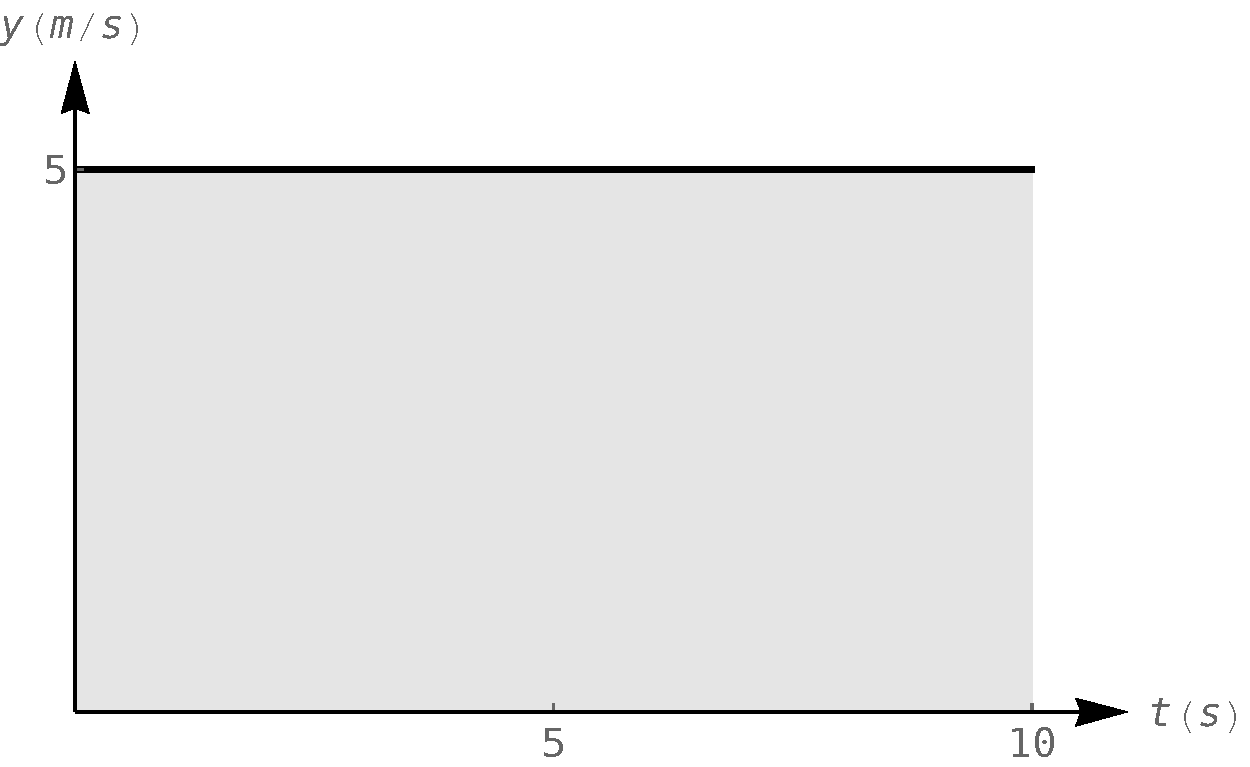
\includegraphics[width=0.43\textwidth]{fig_int_1a}}
\qquad
\subfigure[\label{fig_int_1b}]{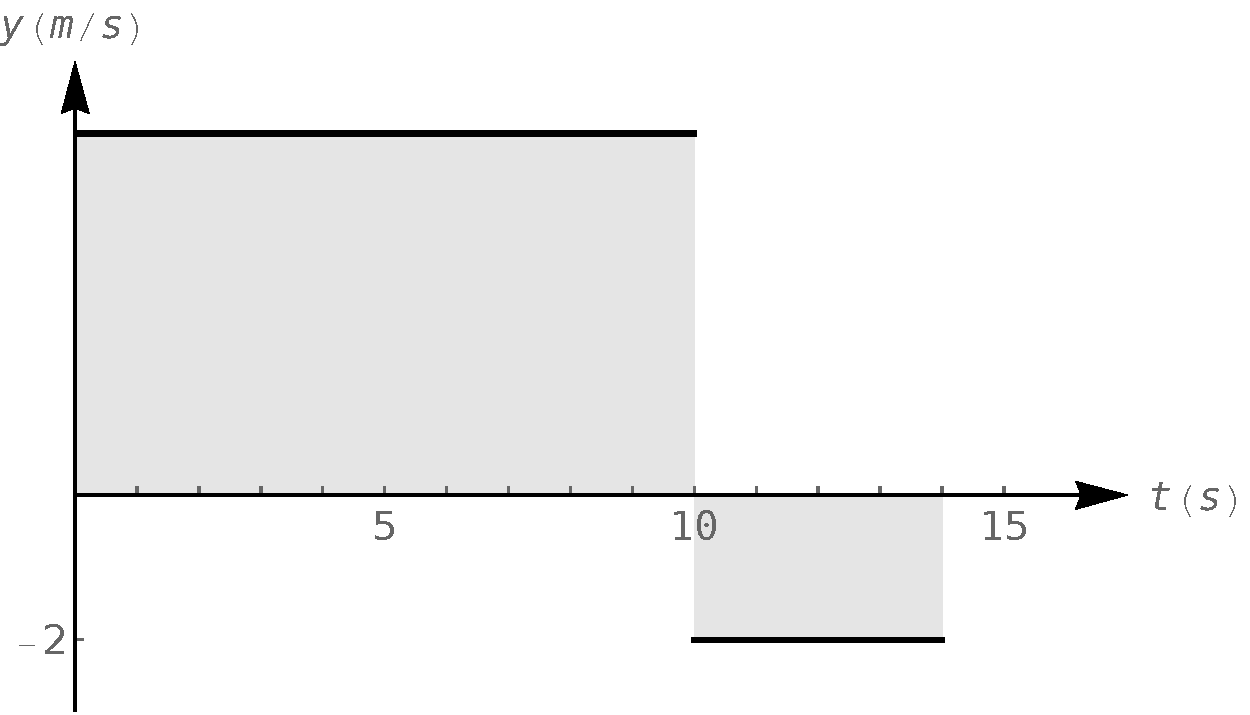
\includegraphics[width=0.43\textwidth]{fig_int_1b} }
\caption{The total displacement of an object travelling in a straight line at a constant velocity of 5m/s for 10 seconds (a) and an object  travelling a straight line with a constant velocity of 5m/s for 10 seconds, and then instantly reversing course at a rate of 2m/s for 4 seconds (b). }
\end{figure}\fi

\ifcalculus\begin{figure}[h]
\centering
%\raisebox{0.5cm}{
\subfigure[\label{fig_int_1a}]{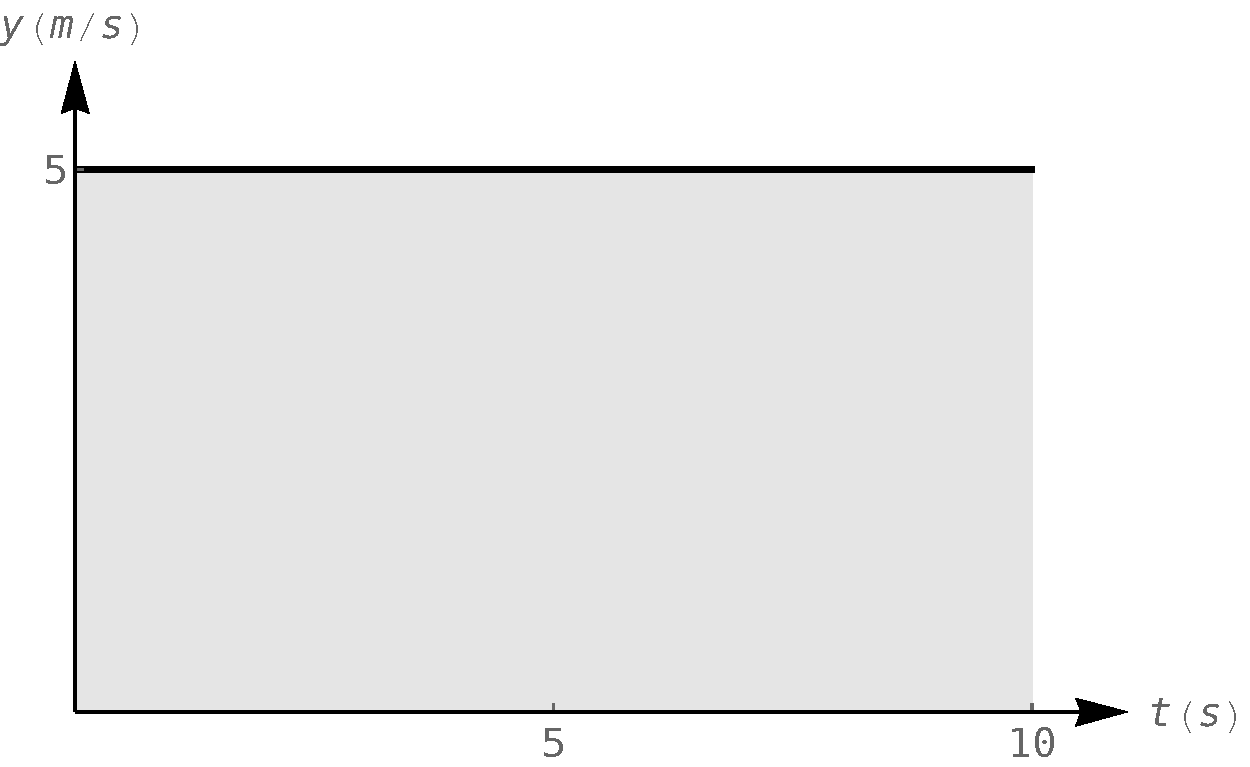
\includegraphics[width=0.43\textwidth]{fig_int_1a}}
\qquad
\subfigure[\label{fig_int_1b}]{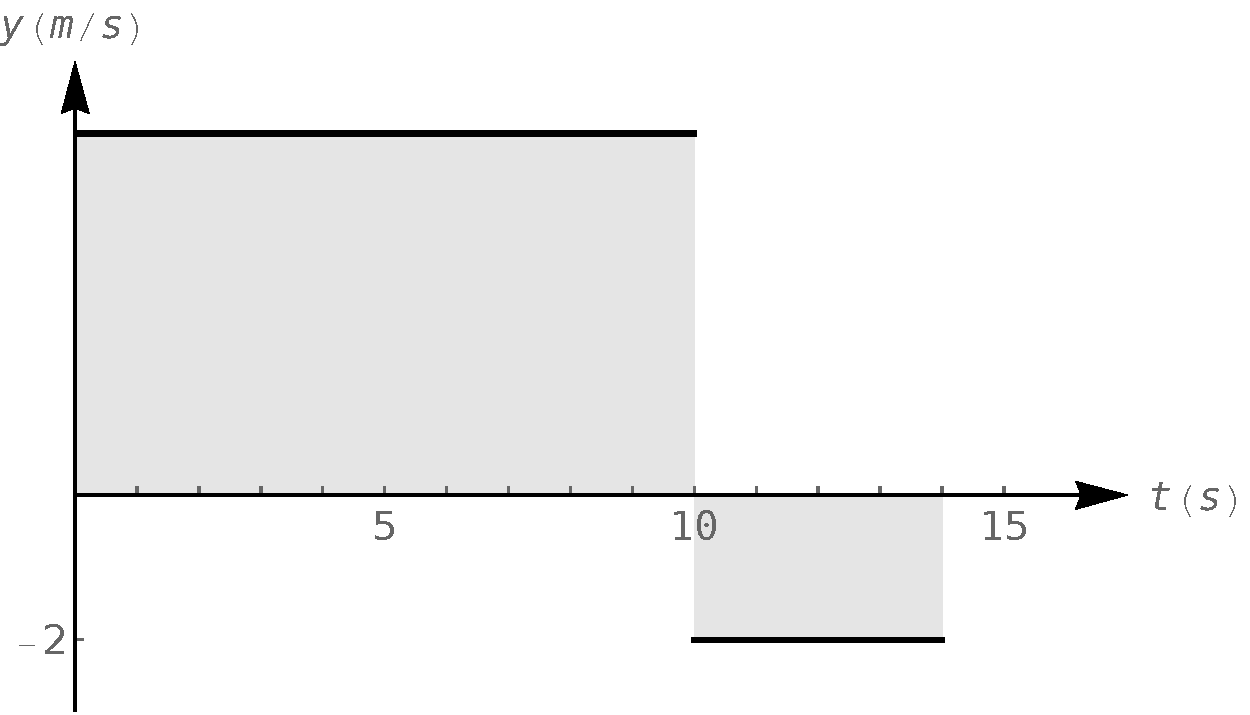
\includegraphics[width=0.43\textwidth]{fig_int_1b} }
\caption{The total displacement of an object travelling in a straight line at a constant velocity of 5m/s for 10 seconds (a) and an object  travelling a straight line with a constant velocity of 5m/s for 10 seconds, and then instantly reversing course at a rate of 2m/s for 4 seconds (b). }
\end{figure}
\fi

Now consider a slightly harder situation (and not particularly realistic): an object travels in a straight line with a constant velocity of 5m/s for 10 seconds, then instantly reverses course at a rate of 2m/s for 4 seconds.  How far away from the starting point is the object -- what is its displacement?

Here, we get:
	$$\text{Distance } \ = 5\cdot10 + (-2)\cdot 4 = 42\text{ m.}$$ 
Hence the object is 42 metres from its starting location.

\ifanalysis\pagebreak\fi
We can again depict this situation graphically. In Figure \ref{fig_int_1b} we have the velocities graphed as straight lines on $[0,10]$ and $[10,14]$, respectively. The displacement of the object is given by  
		\begin{center}Area above the $t$--axis \quad $-$\quad Area below the $t$--axis,
		\end{center}
which is easy to calculate as $50-8=42$ metres.

These examples do not prove a relationship between area under a velocity function and displacement, but it does imply a relationship exists. Section~\ref{sec:FTC} will fully establish fact that the area under a velocity function is displacement.


Anyhow, given a graph of a function $y=f(x)$, we will find that there is great use in computing the area between the curve $y=f(x)$ and the $x$-axis. Because of this, we need to define some terms.

\begin{definition}[The definite integral, total signed area]\label{def:def_int}
Let $y=f(x)$ be defined on a closed interval $[a,b]$. The total signed area from $x=a$ to $x=b$ between $f$ and the $x$-axis  is:\index{integration!definite}\index{definite integral}\index{signed area}\index{total signed area}\index{integration!area}

\centering (area  under $f$ and above the $x$--axis on $[a,b]$) $-$ (area above $f$ and under the $x$--axis on $[a,b]$).\\
\vspace{0.25cm}
\raggedright
The \textbf{definite integral} (\textit{bepaalde integraal}) of $f$ on $[a,b]$ is the total signed area of $f$ on $[a,b]$, denoted $$\ds\int\limits_a^b f(x)\ dx,$$
where $a$ and $b$ are the bounds of integration.
\end{definition}
\index[aut]{integraal ! bepaalde}\index[aut]{integratiegrenzen}

By our definition, the definite integral gives the signed area under $f$. We usually drop the word signed when talking about the definite integral, and simply say the definite integral gives the area under $f$\, or, more commonly, the area under the curve. The indefinite integral and definite integral are very much related, as we will see in Section \ref{sec:FTC}. 

Let us now practice this definition. 

\begin{example}\label{ex_defint4}
Consider the function $f$ given in Figure \ref{fig_int_2}.

\begin{figure}[H]
	\begin{center}
			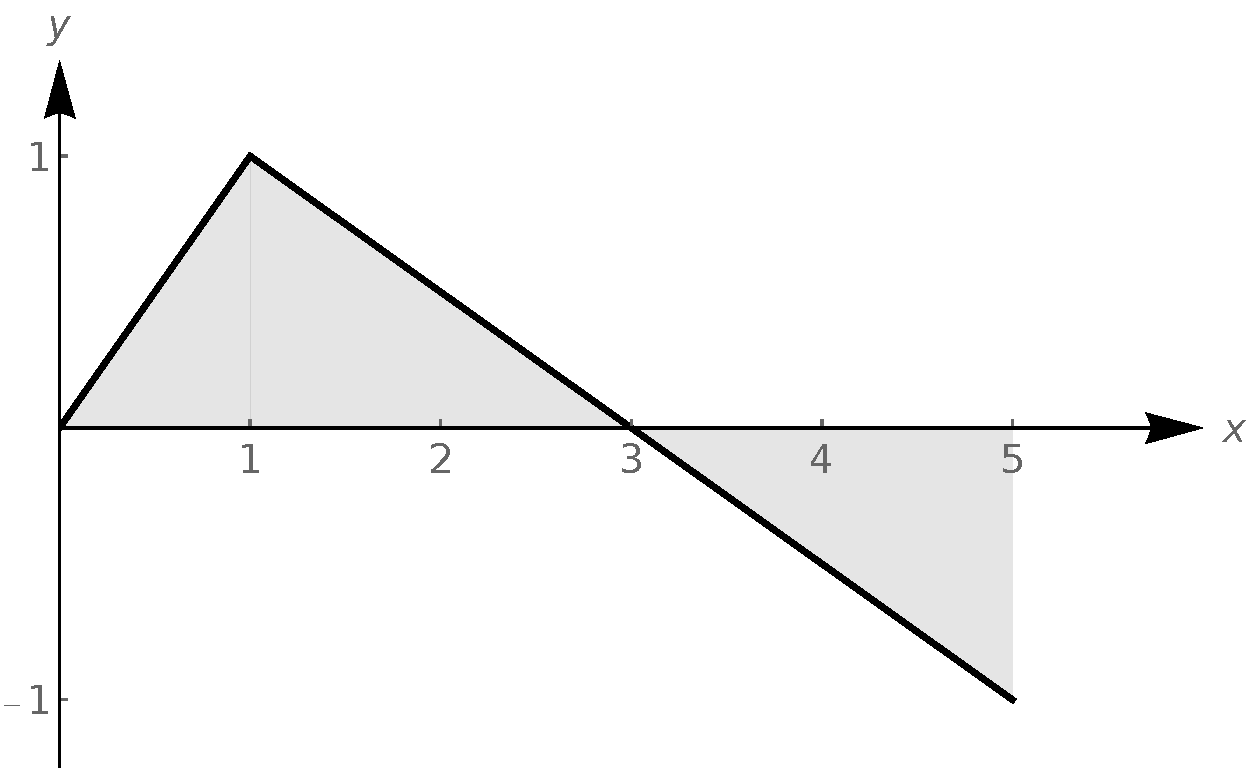
\includegraphics[width=0.5\textwidth]{fig_int_2}
	\caption{A graph of $f(x)$ in Example \ref{ex_defint4}.}
	\label{fig_int_2}
	\end{center}
\end{figure}

\ifanalysis\pagebreak\fi
 Find:

\begin{multicols}{3}
\begin{enumerate}
		\item		$\ds \int\limits_0^3 f(x)\ dx$
		\item		$\ds \int\limits_3^5 f(x)\ dx$
		\item		$\ds \int\limits_0^5 f(x)\ dx$
		\item		$\ds \int\limits_0^3 5f(x)\ dx$
		\item		$\ds \int\limits_1^1 f(x) \ dx$
\end{enumerate}
\end{multicols}


\xhrulefill{gray}{2.5pt}Solution \xhrulefill{gray}{2.5pt}

\begin{enumerate}
		\item	This definite integral is the area under $f$ on the interval $[0,3]$. This region is a triangle, so the area is 
		$$\ds \int\limits_0^3 f(x)\ dx=\frac12(3)(1) = 1.5.$$ 
		\item		This definite integral  represents the area of the triangle found under the $x$--axis on $[3,5]$. The area is $1/2(2)(1) = 1$; since it is found under the $x$--axis, this is negative area. So, 
		$$ \ds \int\limits_3^5 f(x)\ dx = -1.$$
		\item		This definite integral  is the total signed area under $f$ on $[0,5]$. This is $1.5 + (-1) = 0.5$.
		\item		This definite integral is the area under $5f$ on $[0,3]$. Again, the region is a triangle, with height 5 times that of the height of the original triangle. Thus the area is $$\ds \int\limits_0^35f(x)\ dx = \frac12(15)(1) = 7.5.$$
		
		\item		This definite integral  is the area under $f$ on the interval $[1,1]$. This describes a line segment, not a region; it has no width. Therefore the area is 0.
\end{enumerate}
\end{example}

This example illustrates some of the properties of the definite integral, listed in the following theorem.

\begin{theorem}[Properties of the definite integral]\label{thm:defintprop}
Let $f$ and $g$ be defined on a closed interval $I$ that contains the values $a$, $b$ and $c$, and let $k$ be a constant. The following hold:
		\begin{enumerate}
		\item		$\ds \int\limits_a^a f(x)\ dx = 0,$
		\item		$\ds \int\limits_a^b f(x)\ dx + \int\limits_b^c f(x)\ dx = \int\limits_a^cf(x)\ dx,$
		\item		$\ds \int\limits_a^bf(x)\ dx = -\int\limits_b^a f(x)\ dx,$
		\item		$\ds \int\limits_a^b\big(f(x)\pm g(x)\big)\ dx = \int\limits_a^bf(x)\ dx \pm \int\limits_a^bg(x)\ dx,$
		\item		$\ds \int\limits_a^bk\, f(x)\ dx = k\cdot\int\limits_a^bf(x)\ dx.$
		\end{enumerate}
\end{theorem}

\ifanalysis

The proofs of these properties will be provided at the end of the next section once we have a better understanding of definite integrals through the conceptualisation of Riemann sums.

\fi
The area definition of the definite integral allows us to use geometry to compute the definite integral of some simple functions.\\

\begin{example}\label{ex_defint8}
Evaluate the following definite integrals:
\begin{multicols}{2}
\begin{enumerate}
    \item $\ds\int\limits_{-2}^5 (2x-4)\ dx $
    \item $ \ds\int\limits_{-3}^3 \sqrt{9-x^2}\ dx.$
\end{enumerate}
\end{multicols}



\xhrulefill{gray}{2.5pt}Solution \xhrulefill{gray}{2.5pt}

\begin{enumerate}
		\item		It is useful to sketch the function in the integrand, as shown in Figure \ref{fig_int_3a}. We see we need to compute the areas of two regions, which we have labelled $R_1$ and $R_2$. Both are triangles, so the area computation is straightforward:
			$$R_1:\; \frac12(4)(8) = 16 \qquad \qquad R_2:\; \frac12(3)6 = 9.$$ 
Region $R_1$ lies under the $x$--axis, hence it is counted as negative area, so $$\int\limits_{-2}^5(2x-4)\ dx = -16+9 = -7.$$
\ifmathematica
We may check this answer in Mathematica as follows
	\begin{mdframed}[default,backgroundcolor=gray!40,roundcorner=8pt]
\begin{mmaCell}[morefunctionlocal={x}]{Input}
  Integrate[2*x-4, {x,-2,5}]
\end{mmaCell}

\begin{mmaCell}{Output}
   -7
\end{mmaCell}
\end{mdframed}
\index{\lstinline{Integrate}}\index[aut]{\lstinline{Integrate}}
\fi
\ifpython
We may check this answer in Mathematica as follows
\begin{pyin}
from sympy import symbols, integrate
x = symbols('x')
integrate(2*x - 4, (x, -2, 5))
\end{pyin}
\begin{pyout}
-7
\end{pyout}
\fi

\begin{figure}[H]
\centering
%\raisebox{0.5cm}{
\subfigure[\label{fig_int_3a}]{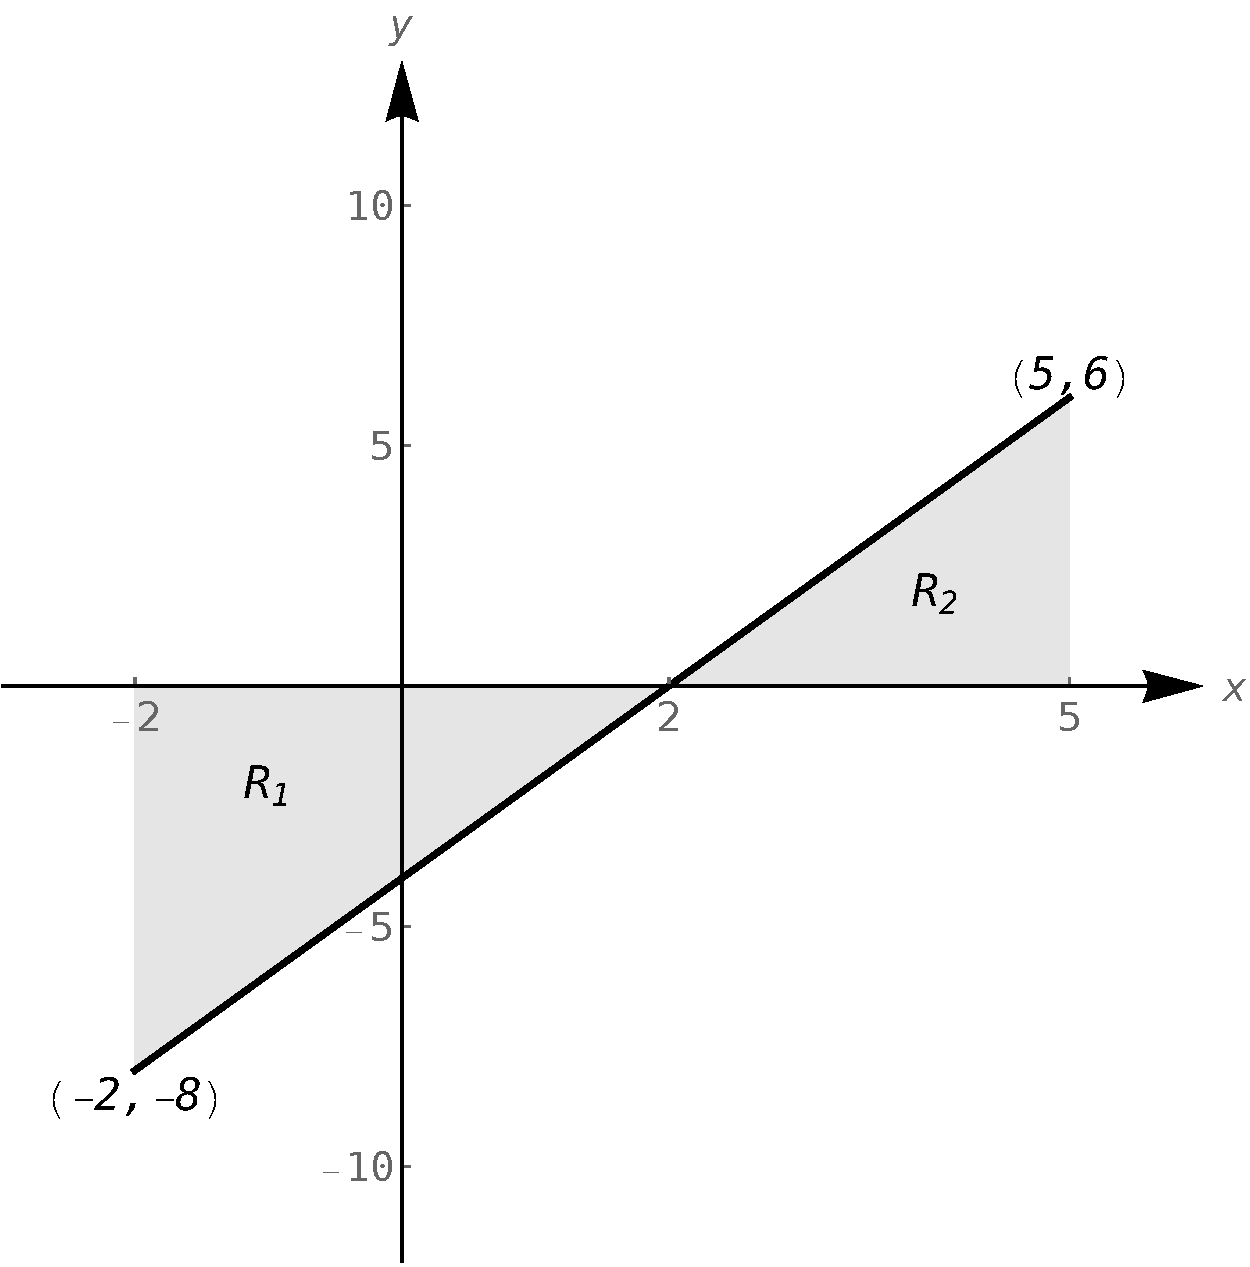
\includegraphics[width=0.43\textwidth]{fig_int_3a}}
\qquad
\subfigure[\label{fig_int_3b}]{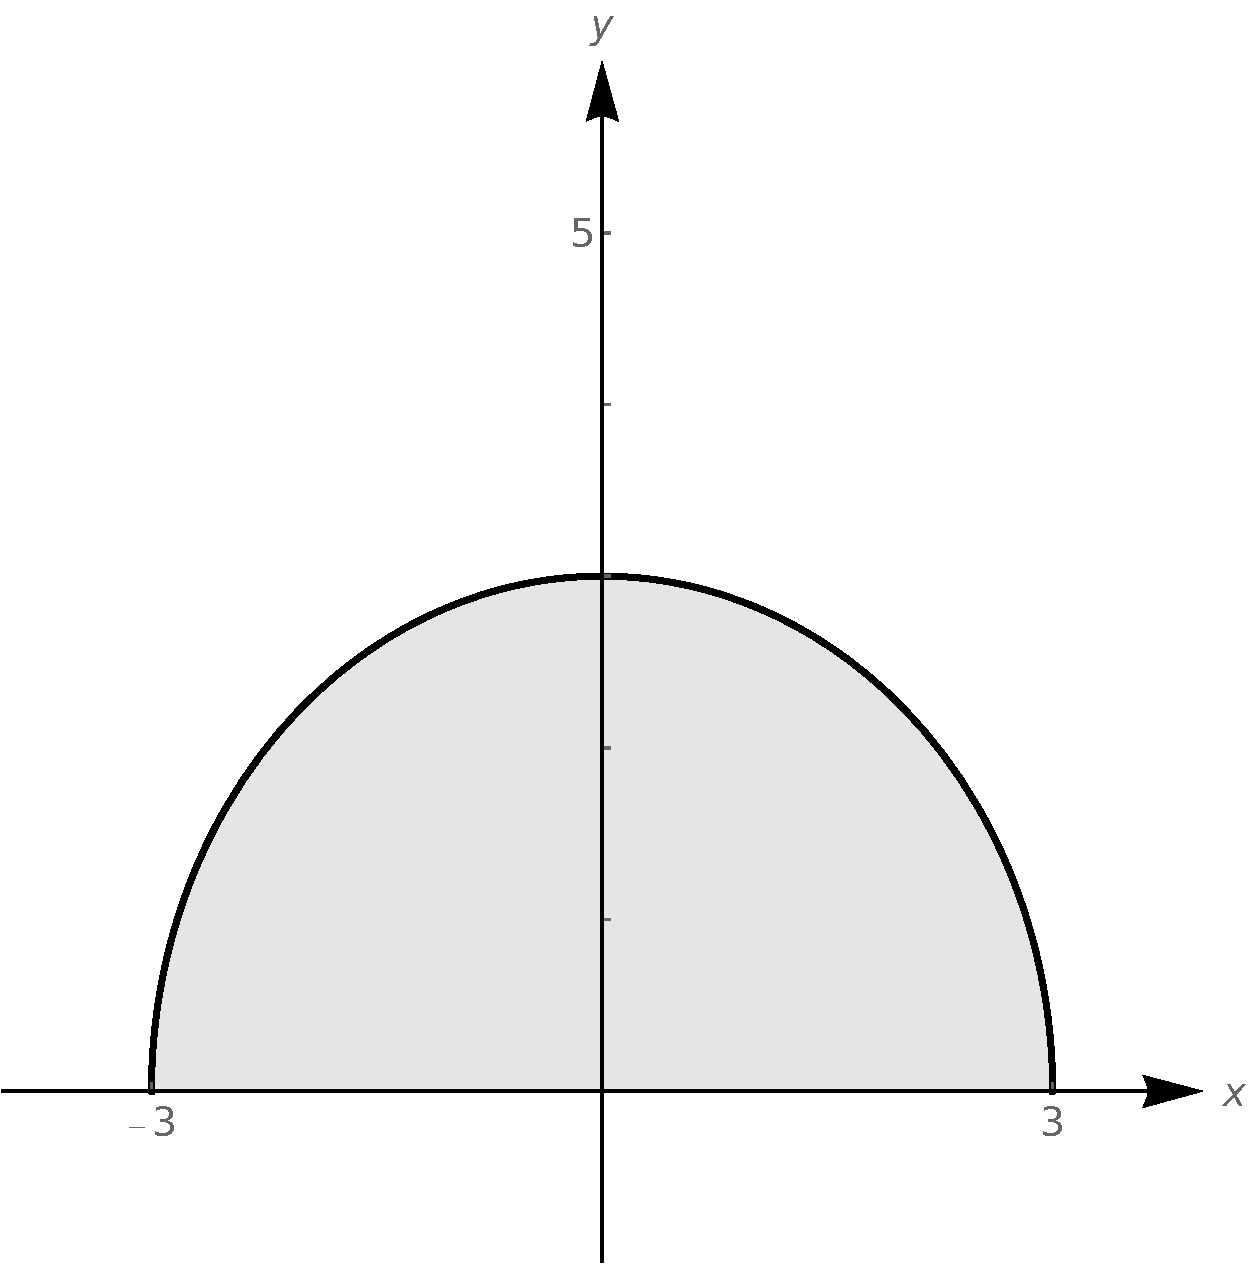
\includegraphics[width=0.43\textwidth]{fig_int_3b} }
\caption{A graph of $f(x) = 2x-4$ in (a) and $f(x) = \sqrt{9-x^2}$ in (b), from Example \ref{ex_defint8}.}
\end{figure}

		\item		Recognize that the integrand of this definite integral describes a half circle, as sketched in Figure \ref{fig_int_3b}, with radius 3. Thus the area is:
		$$\int\limits_{-3}^3 \sqrt{9-x^2}\ dx = \frac12\pi r^2 = \frac 92\pi.$$




\end{enumerate}
\end{example}



\section{Riemann sums}\label{sec:riemann}

In our previous examples, we have either found the areas of regions that have nice geometric shapes  or the areas were given to us. But what is, for instance, the area of a region below $y=x^2$? The function $y=x^2$ is relatively simple, yet the shape it defines has an area that is not simple to find geometrically. In this section we will explore how to find the areas of such regions.

\index{Riemann Sum}\index[aut]{Riemann som}

\subsection{Approximating areas}\label{subsec:Approximating_areas}

Consider the region given in Figure \ref{fig_int_4}, which is the area under $y=4x-x^2$ on $[0,4]$. What is the signed area of this region -- i.e., what is $\int_0^4(4x-x^2)\ dx$? We start by approximating. We can surround the region with a rectangle with height and width of 4 and find the area is approximately 16 square units. This is obviously an over--approximation; we are including area in the rectangle that is not under the parabola. 

\begin{figure}[h]
	\begin{center}
			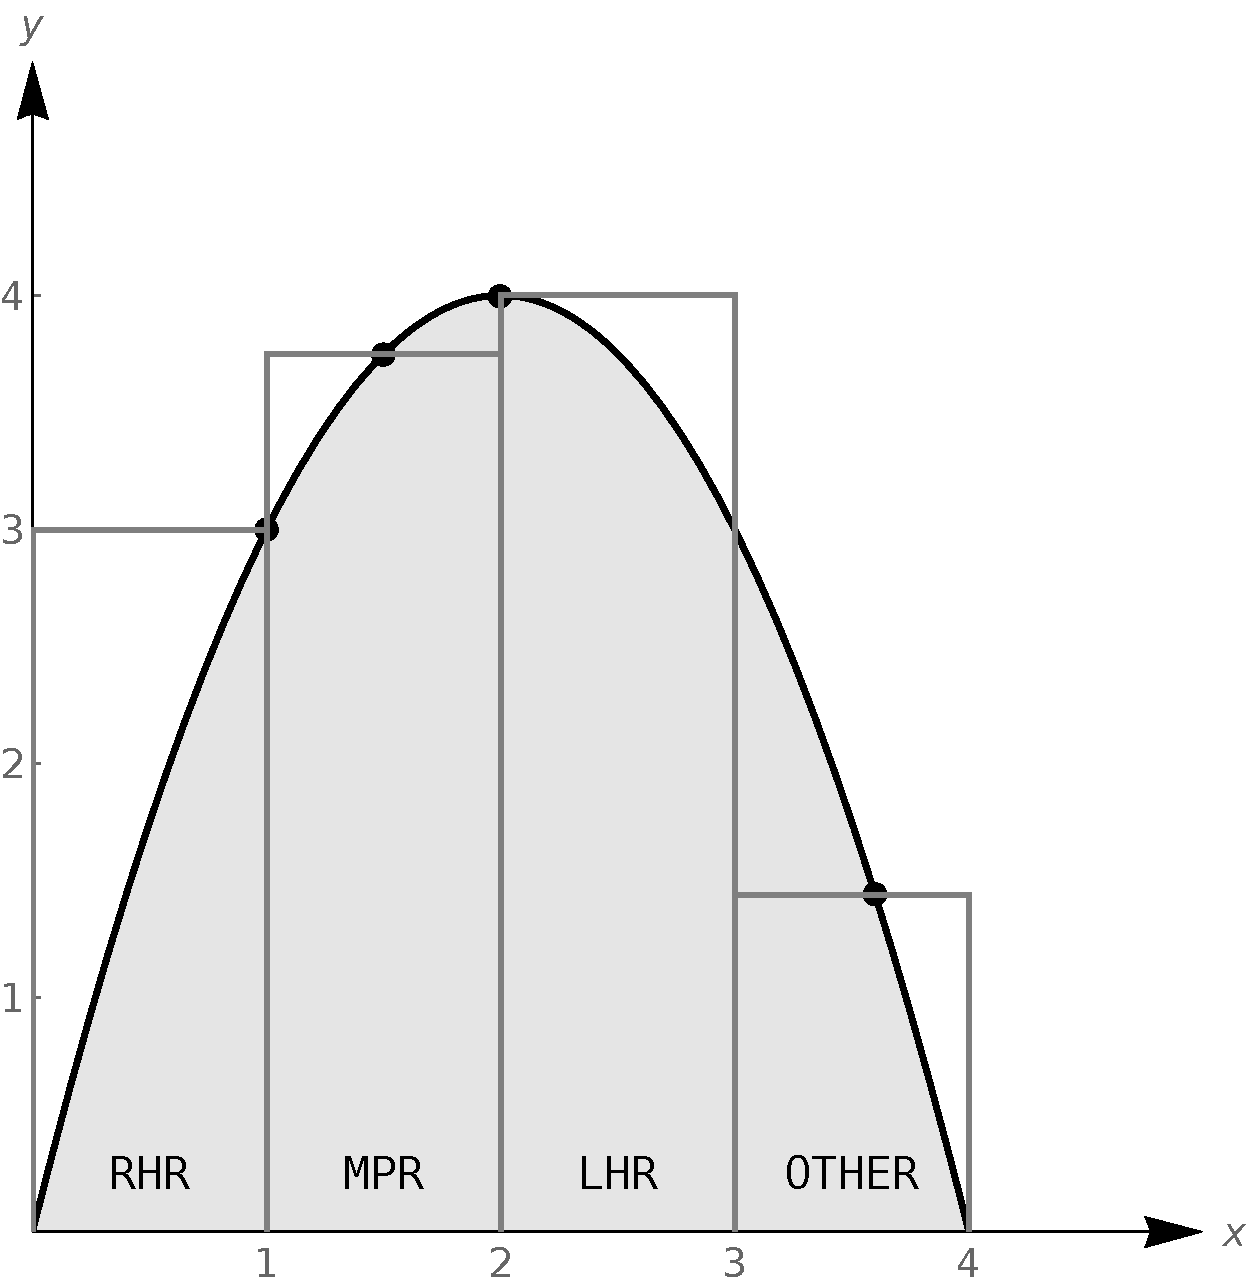
\includegraphics[width=0.4\textwidth]{fig_int_4}
	\caption{A graph of $f(x) = 4x-x^2$ and approximating $\int_0^4(4x-x^2)\ dx$ using rectangles.}
	\label{fig_int_4}
	\end{center}
\end{figure}

We have an approximation of the area, using one rectangle. How can we refine our approximation to make it better? The key to this section is this answer: use more rectangles. Let us use 4 rectangles with an equal width of 1. This partitions the interval $[0,4]$ into 4 subintervals, $[0,1]$, $[1,2]$, $[2,3]$ and $[3,4]$. On each subinterval we will draw a rectangle.

There are three common ways to determine the height of these rectangles: the \textbf{left hand rule} (\textit{linkerhand regel}), the \textbf{right hand rule} (\textit{rechterhand regel}), and the \textbf{midpoint rule} (\textit{midpoint regel}). The left hand rule says to evaluate the function at the left--hand endpoint of the subinterval and make the rectangle that height. In Figure \ref{fig_int_4}, the rectangle drawn on the interval $[2,3]$ has height determined by the left hand rule (LHR); it has a height of $f(2)$. \index{left hand rule}\index{right hand rule}\index{midpoint rule}\index[aut]{midpoint ! regel van intervalmiddens}

The right hand rule (RHR) says the opposite: on each subinterval, evaluate the function at the right endpoint and make the rectangle that height. In  Figure \ref{fig_int_4}, the rectangle drawn on $[0,1]$ is drawn using $f(1)$ as its height. The midpoint rule (MPR) says to evaluate the function at the midpoint of each subinterval, and to make the rectangle that height. The rectangle drawn on $[1,2]$ was made using the midpoint rule, with a height of $f(1.5)$. 

These are the three most common rules for determining the heights of approximating rectangles, but one is not forced to use one of these three methods. The rectangle on $[3,4]$ has a height of approximately $f(3.53)$, very close to the midpoint rule. It was chosen so that the area of the rectangle is exactly the area of the region under $f$ on $[3,4]$.

% The following example will put these rules into practice.%approximate the value of $\ds \int_0^4 (4x-x^2)\ dx$ using these rules.

% \begin{example}\label{ex_rie2}
% Approximate the value of 
% $$\ds \int\limits_{0}^4 (4x-x^2)\ dx$$
% using the left hand rule, the right hand rule, and the midpoint rule, using 4 equally spaced subintervals.

% \xhrulefill{gray}{2.5pt}Solution \xhrulefill{gray}{2.5pt}

% We break the interval $[0,4]$ into four subintervals as before. In Figure \ref{fig_int_5a} we see 4 rectangles drawn on $f(x) = 4x-x^2$ using the left hand rule. The areas of the rectangles are given in each figure.

% %\noindent 
% Note how in the first subinterval, $[0,1]$, the rectangle has height $f(0)=0$. We add up the areas of each rectangle (height$\times$width) for our left hand rule approximation:
% $$f(0)\cdot 1 + f(1)\cdot 1+ f(2)\cdot 1+f(3)\cdot 1 =	0+3+4+3 = 10\,.
% $$
% %	\begin{align*} f(0)\cdot 1 + f(1)\cdot 1+ f(2)\cdot 1+f(3)\cdot 1 &=\\
% %	0+3+4+3&= 10.
% %	\end{align*}
	
% Figure \ref{fig_int_5b} shows 4 rectangles drawn under $f$ using the right hand rule; note how the $[3,4]$ subinterval has a rectangle of height 0. 

% In this example, these rectangles seem to be the mirror image of those found in Figure~\ref{fig_int_5a}. This is because of the symmetry of our shaded region. Our approximation gives the same answer as before, though calculated a different way:
% $$f(1)\cdot 1 + f(2)\cdot 1+ f(3)\cdot 1+f(4)\cdot 1 =
% 	3+4+3+0 = 10\,.$$
% %	\begin{align*} f(1)\cdot 1 + f(2)\cdot 1+ f(3)\cdot 1+f(4)\cdot 1 &=\\
% %	3+4+3+0&= 10.
% %	\end{align*}

% Figure \ref{fig_int_5c} shows 4 rectangles drawn under $f$ using the midpoint rule. This gives :
% $$f(0.5)\cdot 1 + f(1.5)\cdot 1+ f(2.5)\cdot 1+f(3.5)\cdot 1 =
% 	1.75+3.75+3.75+1.75 = 11\,.$$
% %\begin{align*} f(0.5)\cdot 1 + f(1.5)\cdot 1+ f(2.5)\cdot 1+f(3.5)\cdot 1 &=\\
% %	1.75+3.75+3.75+1.75&= 11.
% %	\end{align*}
% Our three methods provide two approximations, namely 10 and 11.

% \begin{figure}[H]
% \centering
% %\raisebox{0.5cm}{
% \subfigure[\label{fig_int_5a}]{\includegraphics[width=0.3\textwidth]{fig_int_5a}}
% \qquad
% \subfigure[\label{fig_int_5b}]{\includegraphics[width=0.3\textwidth]{fig_int_5b} }
% \qquad
% \subfigure[\label{fig_int_5c}]{\includegraphics[width=0.3\textwidth]{fig_int_5c} }
% \caption{Approximating $\int_0^4(4x-x^2)\ dx$ in Example \ref{ex_rie2} using  the left hand rule (a), the right hand rule (b) and the midpoint rule (c).}
% \end{figure}



% \end{example}


It is hard to tell at this moment which is a better approximation. We can continue to refine our approximation by using more rectangles.

\subsection{Riemann sums}
Consider again $\int_0^4(4x-x^2)\ dx$. 
%We will now approximate this definite integral using 16 equally spaced subintervals and the right hand rule in Example \ref{ex_rie7}.
We divide or partition the number line of $[0,4]$ into 16 equally spaced subintervals. We denote $0$ as $x_1$
%; we have marked the values of $x_5$, $x_9$, $x_{13}$ and $x_{17}$. So, 
, so in general, we have
$$x_i = x_1 + (i-1)\Delta x\,,$$
where $i=1,2,\ldots,16$ For the sake of simplicity, we will often write $\Delta x=\Delta x_i$, where $\Delta x_i$ is the width of the $i^\text{ th}$ subinterval, whenever the width of the subintervals is the same. 

Given any subdivision of $[0,4]$, the first subinterval is $[x_1,x_2]$; the second is $[x_2,x_3]$; the $i^\text{ th}$ subinterval is $[x_i,x_{i+1}]$. Hence, when using the left hand rule, the height of the $i^\text{ th}$ rectangle will be $f(x_i)$. When using the right hand rule, the height of the $i^\text{ th}$ rectangle will be $f(x_{i+1})$, and finally, when using the midpoint rule, the height of the $i^\text{ th}$ rectangle will be 
$$\ds f\left(\frac{x_i+x_{i+1}}2\right).$$ 


We illustrate this in the next example.

\begin{example}\label{ex_rie7}
Approximate 
$$\ds\int\limits_0^4(4x-x^2)\ dx$$
 using the right hand rule with 16 and 1000 equally spaced intervals.

\xhrulefill{gray}{2.5pt}Solution \xhrulefill{gray}{2.5pt}

Using 16 equally spaced intervals and the right hand rule, we can approximate the definite integral as $$\sum_{i=1}^{16}f(x_{i+1})\Delta x,$$
where we have $\Delta x = 4/16 = 0.25$. Moreover, since $x_1=0$, we have 
\begin{align*}
x_{i+1} &= 0 + \big((i+1)-1\big)\Delta x \\
				&=	i\Delta x\,.
\end{align*}
%In our examples using the right hand rule is simpler notationally as $f(x_{i+1}) = f(i\Delta x)$. 

Using summation formulas, we may now consider:
\allowdisplaybreaks
\begin{align}
\ds\int\limits_0^4 (4x-x^2)\ dx &\approx \sum_{i=1}^{16} f(x_{i+1})\Delta x = \sum_{i=1}^{16} f(i\Delta x) \Delta x \notag\\[0.2cm]
                                    &= \sum_{i=1}^{16} \big(4i\Delta x - (i\Delta x)^2\big)\Delta x = \sum_{i=1}^{16} (4i\Delta x^2 - i^2\Delta x^3)\notag\\[0.2cm] 
									&= (4\Delta x^2)\sum_{i=1}^{16} i - \Delta x^3 \sum_{i=1}^{16} i^2 \label{eq:rie7}\\[0.2cm]
									&= (4\Delta x^2)\frac{16\cdot 17}{2} - \Delta x^3 \frac{16(17)(33)}6=10.625 &\quad \text{ $(\Delta x = 0.25)$}\notag\\[0.2cm]
									%&=	4\cdot 0.25^2\cdot 136-0.25^3\cdot 1496\notag\\
									%&=10.625\,.\notag
\end{align}
We were able to sum up the areas of 16 rectangles with very little computation. In Figure \ref{fig_int_5} the function and the 16 rectangles are graphed. While some rectangles over--approximate the area, other under--approximate the area by about the same amount. Thus our approximate area of 10.625 is likely a fairly good approximation.


For what concerns the approximation based on 1000 equally spaced, we can just use Equation \eqref{eq:rie7}; after replacing the 16's to 1000's and appropriately changing the value of $\Delta x$.
%\drawexampleline

%\enlargethispage{\baselineskip}
We do so here, skipping from the original summand to the equivalent of Equation \eqref{eq:rie7} to save space. Note that $\Delta x = 4/1000 = 0.004$.

\begin{align}
\ds\int\limits_0^4 (4x-x^2)\ dx &\approx \sum_{i=1}^{1000} f(x_{i+1})\Delta x \notag\\
									&= (4\Delta x^2)\sum_{i=1}^{1000} i - \Delta x^3 \sum_{i=1}^{1000} i^2 \notag\\
									&= (4\Delta x^2)\frac{1000\cdot 1001}{2} - \Delta x^3 \frac{1000(1001)(2001)}6 \notag\\
									%&=	4\cdot 0.004^2\cdot 500500-0.004^3\cdot 333,833,500\notag\\
									&=10.666656 \notag
\end{align}


\begin{figure}[H]
	\begin{center}
			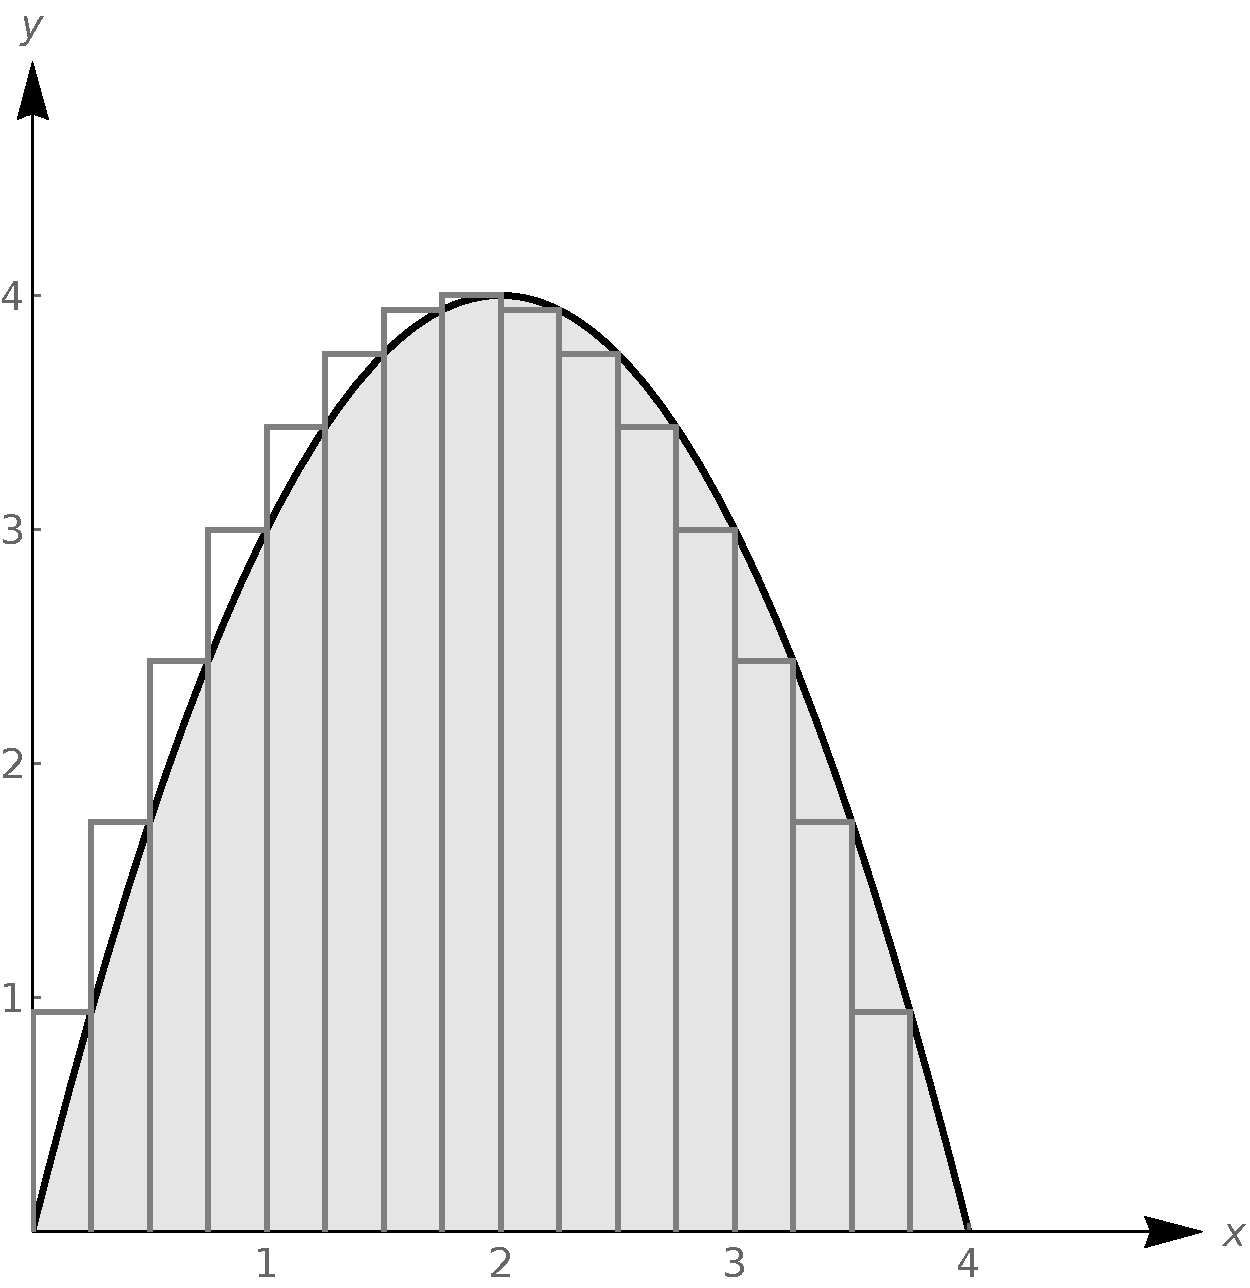
\includegraphics[width=0.4\textwidth]{fig_int_5}
	\caption{Approximating $\int_0^4(4x-x^2)\ dx$ with the right hand rule and 16 evenly spaced subintervals.}
	\label{fig_int_5}
	\end{center}
\end{figure}


Using many, many rectangles, we have a likely good approximation of 

$\int_0^4 (4x-x^2)\dx$. That is, $$\int_0^4(4x-x^2)\ dx \approx 10.666656.$$
\end{example}

Instead of approximating a definite integral using rectangles of the same width and height determined by evaluating $f$ at a particular point in each consecutive subinterval, we could partition an interval $[a,b]$ with subintervals that do not have the same size. We refer to the length of the $i^\text{ th}$ subinterval as $\Delta x_i$. Also, one could determine each rectangle's height by evaluating $f$ at any point $c_i$ in the $i^\text{ th}$ subinterval. Thus the height of the $i^\text{ th}$ subinterval would be $f(c_i)$, and the area of the $i^\text{ th}$ rectangle would then be $f(c_i)\Delta x_i$.

These ideas are formally defined below.
%\enlargethispage{4\baselineskip}

\begin{definition}[Partition]\label{def:partition}
A \textbf{partition} (\textit{partitie}) of a closed interval $[a,b]$ is a set of numbers $x_1$, $x_2$, $\ldots$ $x_{n+1}$ where 
$$a=x_1 < x_2 < \ldots < x_n < x_{n+1}=b.$$
The length of the $i^\text{ th}$ subinterval, $[x_i,x_{i+1}]$, is $\Delta x_i = x_{i+1}-x_i$. If $[a,b]$ is partitioned into subintervals of equal length, we let $\Delta x_i$ represent the length of each subinterval.\\

The size of the partition, denoted $\mathcal{L}$, is the length of the largest subinterval of the partition, i.e. $\mathcal{L}=\max\limits_i\left(\Delta x_i\right)$.\index{partition}\index{partition ! size of}\index[aut]{partitie}
\end{definition}

Summations of rectangles with area $f(c_i)\Delta x_i$ are named after mathematician Georg Friedrich Bernhard Riemann, as given in the following definition.

\begin{definition}[Riemann sum]\label{def:rie_sum}
Let $f$ be defined on a closed interval $[a,b]$, let $\{x_1,\,x_2,\ldots,x_{n+1}\}$ be a partition of $[a,b]$ \index{Riemann Sum}\index[aut]{Riemann som}

and let $c_i$ denote any value in the $i^\text{ th}$ subinterval.

The sum $$\sum_{i=1}^n f(c_i)\Delta x_i$$  is a \textbf{Riemann sum} (\textit{Riemann som}) of $f$ on $[a,b]$.
\end{definition}



Usually Riemann sums are calculated using one of the three methods we have introduced. The uniformity of construction  makes computations easier. So 
$$\ds\int\limits_a^b f(x) \ dx$$
is typically approximated by means of the following Riemann sum
$$
\sum_{i=1}^n f(c_i)\Delta x_i\,,
$$
for which we take the following steps. 
\begin{enumerate}
\item	Divide the interval $[a,b]$ in $n$ subintervals have equal length, such that
$$\ds \Delta x_i = \Delta x = \frac{b-a}n$$
and the $i^\text{ th}$ term of the equally spaced partition is 
$$x_i = a + (i-1)\Delta x\,.$$ Thus $x_1=a$ and  $x_{n+1} = b\,.$

\item Evaluate one of the following summations:
\begin{enumerate}
\item		using the left hand rule we get the so-called \textbf{left Riemann sum} (\textit{linker Riemann som}):
$$\ds \sum_{i=1}^n f(x_i)\Delta x,$$
\item		using the right hand rule we get the so-called \textbf{right Riemann sum} (\textit{rechter Riemann som}): 
$$\ds \sum_{i=1}^n f(x_{i+1})\Delta x,$$
\item		and using the midpoint rule we get the \textbf{middle Riemann sum} (\textit{midden Riemann som}):
$$\ds \sum_{i=1}^n f\left(\frac{x_i+x_{i+1}}{2}\right)\Delta x\,.$$
\end{enumerate}
\end{enumerate}

% \begin{example}\label{ex_rie8}
% Approximate $$\ds\int\limits_{-2}^3 (5x+2)\ dx$$ using the midpoint rule and 10 equally spaced intervals.


% \xhrulefill{gray}{2.5pt}Solution \xhrulefill{gray}{2.5pt}


% We have $\Delta x = 1/2$ and  $x_i = (-2) + (1/2)(i-1) = i/2-5/2$ for $i=1,2,\ldots,10$.  	As we are using the midpoint rule, we will also need $x_{i+1}$ and $ \frac{x_i+x_{i+1}}2$: 
% 	$$\frac{x_i+x_{i+1}}2 = \frac{(i/2-5/2) + \left((i+1)/2-5/2\right)}{2} = \frac{i-9/2}{2} = \dfrac{i}{2} - \dfrac{9}{4}.$$
% 	We now construct the Riemann sum and compute its value.
% 	\allowdisplaybreaks
% \begin{align*}
% \ds\int\limits_{-2}^3 (5x+2)\ dx 	&\approx \sum_{i=1}^{10} f\left(\frac{x_i+x_{i+1}}{2}\right)\Delta x \\[0.2cm]
% 												&=	\sum_{i=1}^{10} f\left(\dfrac{i}{2} - \dfrac{9}{4}\right)\Delta x \\[0.2cm]
% 												&=	\sum_{i=1}^{10} \left(5\left(\dfrac{i}{2} - \dfrac{9}{4}\right) + 2\right)\Delta x\\[0.2cm]
% 												&=	\Delta x\sum_{i=1}^{10}\left[\left(\frac{5}{2}\right)i - \frac{37}{4}\right]\\[0.2cm]
% 												&=	\Delta x\left(\frac{5}2\sum_{i=1}^{10} (i) - \sum_{i=1}^{10}\left(\frac{37}{4}\right)\right) \\[0.2cm]
% 												&= \frac12\left(\frac52\cdot\frac{10(11)}{2} - 10\cdot\frac{37}4\right)  \\[0.2cm]
% 												&= \frac{45}2 = 22.5
% \end{align*}


% Note the graph of $f(x) = 5x+2$ in Figure \ref{fig_int_7}. The regions whose area is computed by the definite integral are triangles, meaning we can find the exact answer without summation techniques. We find that the exact answer is indeed 22.5. One of the strengths of the midpoint rule is that often each rectangle includes area that should not be counted, but misses other area that should. When the partition size is small, these two amounts are about equal and these errors almost cancel each other out. In this example, since our function is a line, these errors are exactly equal and they do cancel each other out, giving us the exact answer.

% Note too that when the function is negative, the rectangles have a negative height. When we compute the area of the rectangle, we use $f(c_i)\Delta x$; when $f$ is negative, the area is counted as negative.

% \begin{figure}[H]
% 	\begin{center}
% 			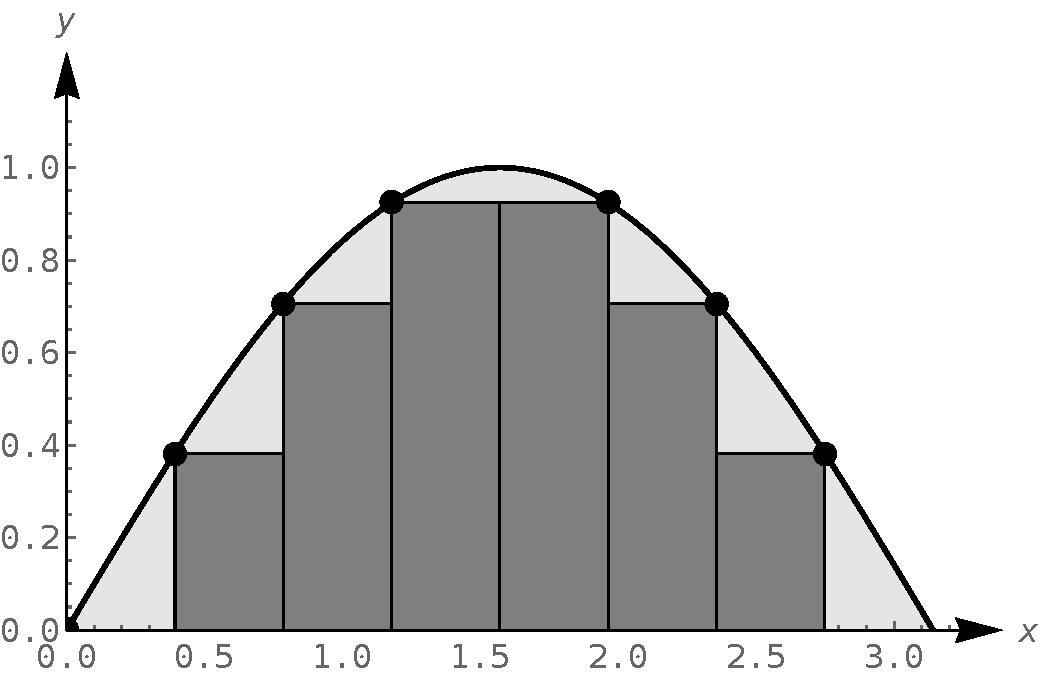
\includegraphics[width=0.5\textwidth]{fig_int_7}
% 	\caption{Approximating $ \int_{-2}^3 (5x+2)\ dx$ using the midpoint rule and 10 evenly spaced subintervals in Example \ref{ex_rie8}.}
% 	\label{fig_int_7}
% 	\end{center}
% \end{figure}


% \end{example}

% Notice in the previous example that while we used 10 equally spaced intervals, this number did not play a big role in the calculations until the very end. Mathematicians love to abstract ideas; let us approximate the area of another region using $n$ subintervals, where we do not specify a value of $n$ until the very end.

\ifanalysis
\begin{example}\label{ex_rie9}

Revisit $$\ds\int\limits_0^4(4x-x^2)\ dx$$ yet again. Approximate this definite integral using the right hand rule with $n$ equally spaced subintervals.

\xhrulefill{gray}{2.5pt}Solution \xhrulefill{gray}{2.5pt}

We know $\Delta x = (4-0)/n = 4/n$. We also find $x_i = 0 + \Delta x(i-1) = 4(i-1)/n$. The right hand rule uses $x_{i+1}$, which is $x_{i+1} = 4i/n$.

We construct the right Riemann sum as follows.
\allowdisplaybreaks
\begin{align*}
		\ds\int\limits_0^4(4x-x^2)\ dx &\approx \sum_{i=1}^n f(x_{i+1})\Delta x \\[0.2cm]
											&= \sum_{i=1}^n f\left(\frac{4i}{n}\right) \Delta x \\[0.2cm]
											&=	\sum_{i=1}^n \left[4\frac{4i}n-\left(\frac{4i}n\right)^2\right]\Delta x\\[0.2cm]
											&=	\sum_{i=1}^n \left(\frac{16\Delta x}{n}\right)i - \sum_{i=1}^n \left(\frac{16\Delta x}{n^2}\right)i^2 \\[0.2cm]
											&=	\left(\frac{16\Delta x}{n}\right)\sum_{i=1}^n i - \left(\frac{16\Delta x}{n^2}\right)\sum_{i=1}^n i^2  \\[0.2cm]
											&= \left(\frac{16\Delta x}{n}\right)\cdot \frac{n(n+1)}{2} - \left(\frac{16\Delta x}{n^2}\right)\frac{n(n+1)(2n+1)}{6} \quad \\[0.2cm]
											&=\frac{32(n+1)}{n} - \frac{32(n+1)(2n+1)}{3n^2} \quad  \\[0.2cm]
											&= \frac{32}{3}\left(1-\frac{1}{n^2}\right)
\end{align*}
%\drawexampleline

The result is an amazing, easy to use formula. To approximate the definite integral with 10 equally spaced subintervals and the right hand rule, set $n=10$ and compute $$\ds\int\limits_0^4 (4x-x^2)\ dx \approx \frac{32}{3}\left(1-\frac{1}{10^2}\right) = 10.56.$$
Recall how earlier we approximated the definite integral with 4 subintervals; with $n=4$, the formula gives 10, our answer as before.

We now take an important leap. More precisely, for any finite $n$, we know that 
$$\ds\int\limits_0^4 (4x-x^2)\ dx \approx \frac{32}{3}\left(1-\frac{1}{n^2}\right)\,.$$ 
Both common sense and high--level mathematics tell us that as $n$ gets large, the approximation gets better. In fact, if we take the limit as $n\rightarrow +\infty$, we get the exact are we are looking for, that is: 
\allowdisplaybreaks
\begin{align*}
\ds\int\limits_0^4 (4x-x^2)\ dx &= \lim_{n\rightarrow +\infty} \frac{32}{3}\left(1-\frac{1}{n^2}\right) \\[0.2cm]
									&= \frac{32}{3}\left(1-0\right)\\[0.2cm]
									&= \frac{32}{3}\,.
\end{align*}
This is a fantastic result. By considering $n$ equally--spaced subintervals, we obtained a formula for an approximation of the definite integral that involved our variable $n$. As $n$ grows large -- without bound -- the error shrinks to zero and we obtain the exact area.
\end{example}

In addition to the left, right and middle Riemann sums, also \textbf{upper and lower Riemann sums} (\textit{boven en onder Riemann som}) can be defined. For that purpose, we consider a partition as before, and note that $f$ has both a minimum and maximum on $[x_i,x_{i+1}]$, so there are numbers $l_i$ and $u_i$ in $[x_i,x_{i+1}]$ such that
$$
f(l_i)\leq f(x)\leq f(u_i)
$$
for all $x$ in $[x_i,x_{i+1}]$. If $f(x)\geq0$, $f(l_i)\Delta x_i$ and $f(u_i)\Delta x_i$ represent the areas of rectangles having the interval $[x_i,x_{i+1}]$ as basis and having tops passing through the lowest and highest points on the graph of $f$ on that interval (Figure~\ref{fig_int_6}). Clearly, if $A_i$ is the area under the graph of $f$ and above the horizontal axis, enclosed between the straight lines $x=x_i$ and $x+x_{i+1}$, then it holds that 
$$
f(l_i)\Delta x_i\leq A_i\leq f(u_i)\Delta x_i.
$$
If $f$ is not restricted to the positive half plan, then either one or both $f(l_i)\Delta x_i$ and $f(u_i)\Delta x_i$ can be negative and will then represent the area of a rectangle lying below the $x$-axis. Anyhow, it will always hold that $f(l_i)\Delta x_i\leq f(u_i)\Delta x_i$.

\begin{figure}
	\begin{center}
			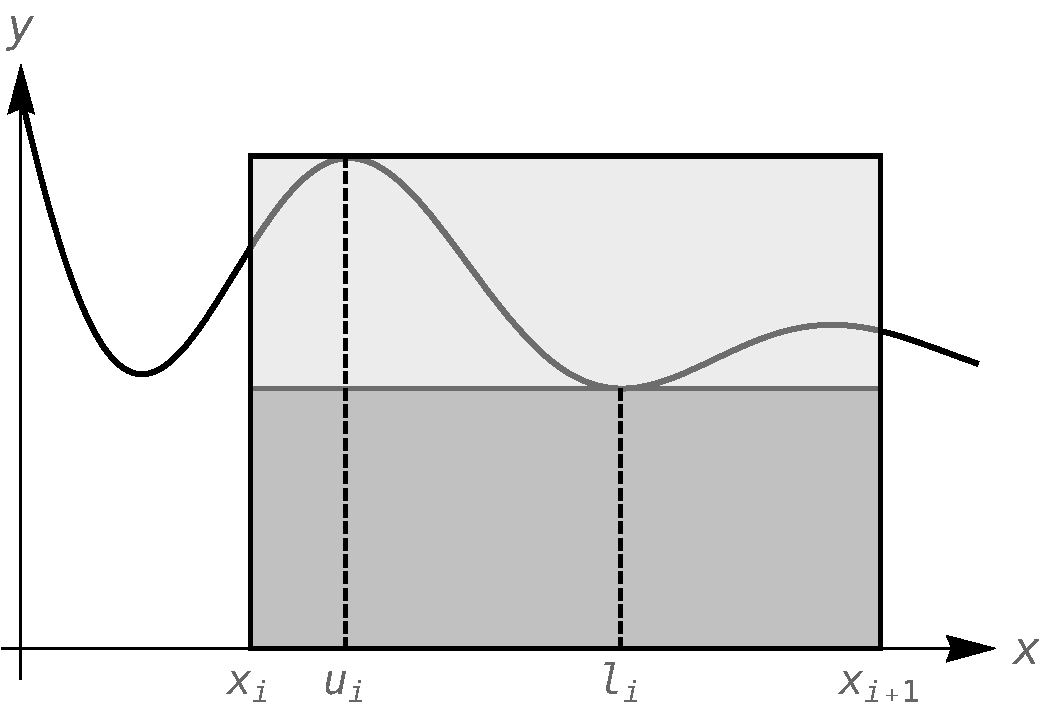
\includegraphics[width=0.5\textwidth]{fig_int_6}
	\caption{$f$ has both a minimum and maximum on $[x_i,x_{i+1}]$.}
	\label{fig_int_6}
	\end{center}
\end{figure}

With this notation in place we can define the lower Riemann sum as
$$\ds S_l(n) = \sum_{i=1}^n f(l_i)\Delta x\,,$$
and the upper Riemann sum as
$$\ds S_u(n) = \sum_{i=1}^n f(u_i)\Delta x\,.$$

To illustrate the subtle difference between the left and lower Riemann sums, on the one hand, and the lower Riemann sum, for instance, on the other hand, consider Figure~\ref{fig_int_7}, where the area under the sine curve between $x=0$ and $x=\pi$ is approximated using the latter. From this figure, it should be clear that lower Riemann sum agrees with the left Riemann sum where the sine is increasing, whereas it corresponds with the right Riemann sum on the interval where the sine curve is decreasing. 

\begin{figure}[h]
	\begin{center}
			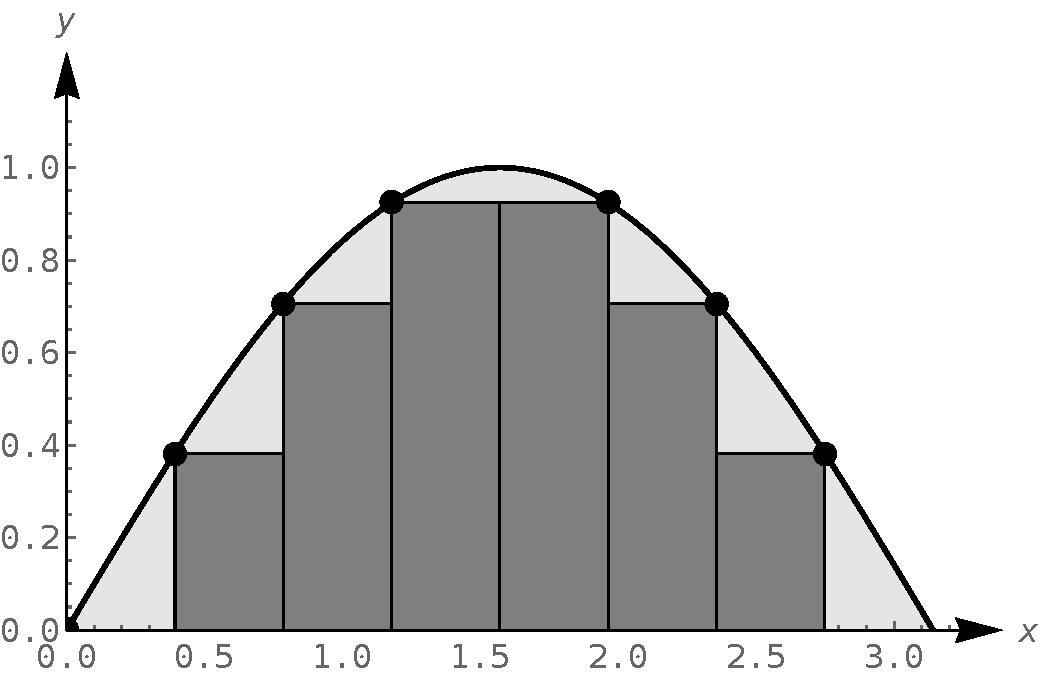
\includegraphics[width=0.5\textwidth]{fig_int_7}
	\caption{Distinction between the left and right Riemann sums and the lower Riemann sum.}
	\label{fig_int_7}
	\end{center}
\end{figure}
\fi

\subsection{Limits of Riemann sums}
We have used limits to evaluate given definite integrals. Will this always work? We will show, given not--very--restrictive conditions, that yes, it will always work.

The previous example has shown us how we can think of a summation as a function of $n$. More precisely, given a definite integral $\int_a^b f(x)\ dx$, we let:
	\begin{itemize}
	\item	$\ds S_L(n) = \sum_{i=1}^n f(x_i)\Delta x$, be the left Riemann sum,
	\item	$\ds S_R(n) = \sum_{i=1}^n f(x_{i+1})\Delta x$, be the right Riemann sum,
	\item	$\ds S_M(n) = \sum_{i=1}^n f\left(\frac{x_i+x_{i+1}}{2}\right)\Delta x$, be the sum of equally spaced rectangles formed using the midpoint rule,
	\end{itemize}
	
and likewise for the lower and upper Riemann sums. Now, recall that the definition of the limit	$\ds\lim_{n\to+\infty}S_L(n) = K$ implies that given any $\epsilon>0$, there exists $N>0$ such that 
		$$\left|S_L(n)-K\right| < \epsilon,$$
when $n\geq N$.

The following theorem states that we can use any of our three rules to find the exact value of a definite integral.

\begin{theorem}[Definite integrals and the limit of Riemann sums]\label{thm:riemann_sum}
Let $f$ be continuous on the closed interval $[a,b]$  and let $S_L(n)$, $S_R(n)$, $S_M(n)$, $\Delta x$, $\Delta x_i$ and $c_i$ be defined as before. Then:\index{Riemann sum}\index[aut]{Riemann som}
\begin{enumerate}
	\item		$\ds \lim_{n\to+\infty} S_L(n) = \lim_{n\to+\infty} S_R(n) = \lim_{n\to+\infty} S_M(n) = \lim_{n\to+\infty}\sum_{i=1}^n f(c_i)\Delta x$, 
	
	\item		$\ds \lim_{n\to+\infty}\sum_{i=1}^n f(c_i)\Delta x = \ds\int\limits_a^b f(x)\ dx$, and %$\ds \lim_{n\to+\infty} S_L(n) = \int_a^b f(x)\ dx$.
	\item		$\ds \lim_{\mathcal{L}\to 0} \sum_{i=1}^n f(c_i)\Delta x_i = \ds\int\limits_a^b f(x)\ dx$.%, where the latter sum is any Riemann sum of $f$ on $[a,b]$, and
\end{enumerate}
\end{theorem}

This theorem also goes two steps further. It states that the height of each rectangle does not have to be determined following a specific rule, but could be $f(c_i)$, where $c_i$ is any point in the $i^\text{ th}$ subinterval. Furthermore, it goes on to state that the rectangles do not need to be of the same width. 

Let $\mathcal{L}$ represent the length of the largest subinterval in the partition: that is, $\mathcal{L}$ is the largest of all the $\Delta x_i$'s. If $\mathcal{L}$ is small, then $[a,b]$ must be partitioned into many subintervals, since all subintervals must have small lengths. Taking the limit as $\mathcal{L}$ goes to zero implies that the number $n$ of subintervals in the partition is growing to infinity, as the largest subinterval length is becoming arbitrarily small. We then interpret the expression 
$$\lim_{\mathcal{L}\to 0}\sum_{i=1}^nf(c_i)\Delta x_i$$
as the limit of the sum of the areas of rectangles, where the width of each rectangle can be different but getting small, and the height of each rectangle is not necessarily determined by a particular rule. The theorem states that this Riemann sum also gives the value of the definite integral of $f$ over $[a,b]$.



\ifanalysis

Having  a better understanding of the definite integral in terms of Riemann sums, we are now ready to prove the properties listed in Theorem~\ref{thm:defintprop}.

\begin{proof}[of Theorem~\ref{thm:defintprop}]
We prove the fourth statement in this theorem, namely that
$$
\displaystyle\int\limits_{{\,a}}^{{\,b}}{{\left(f\left( x \right) \pm g\left( x \right) \right)\,dx}} = \int\limits_{{\,a}}^{{\,b}}{{f\left( x \right)\,dx}} \pm \int\limits_{{\,a}}^{{\,b}}{{g\left( x \right)\,dx}}\,.
$$
The proofs of the other properties proceed in a similar way. 

First we will prove the sum rule. From the definition of the definite integral we have,
\allowdisplaybreaks
\begin{align*}
\int\limits_{{\,a}}^{{\,b}}{{\left(f\left( x \right) + g\left( x \right)\right)\,dx}} & = \mathop {\lim }\limits_{n \to +\infty } \sum\limits_{i = 1}^n {\left( {f\left( {x_i^*} \right) + \,g\left( {x_i^*} \right)} \right)\Delta x} \\ &  = \mathop {\lim }\limits_{n \to +\infty } \left( {\sum\limits_{i = 1}^n {f\left( {x_i^*} \right)\Delta x}  + \sum\limits_{i = 1}^n {g\left( {x_i^*} \right)\Delta x} } \right)\\ &  = \mathop {\lim }\limits_{n \to +\infty } \sum\limits_{i = 1}^n {f\left( {x_i^*} \right)\Delta x}  + \mathop {\lim }\limits_{n \to +\infty } \sum\limits_{i = 1}^n {g\left( {x_i^*} \right)\Delta x} \\ &  = \int\limits_{{\,a}}^{{\,b}}{{f\left( x \right)\,dx}} + \int\limits_{{\,a}}^{{\,b}}{{g\left( x \right)\,dx}}
\end{align*}

To prove the difference formula we can either redo the above work with a minus sign instead of a plus sign or we can use the fact that we now know this is true with a plus and using the properties proved above as follows.
\begin{align*}
\int\limits_{{\,a}}^{{\,b}}{{\left(f\left( x \right) - g\left( x \right)\right)\,dx}} & = \int\limits_{{\,a}}^{{\,b}}{{f\left( x \right) + \left( { - g\left( x \right)} \right)\,dx}}\\ &  = \int\limits_{{\,a}}^{{\,b}}{{f\left( x \right)\,dx}} + \int\limits_{{\,a}}^{{\,b}}{{\left( { - g\left( x \right)} \right)\,dx}}\\ &  = \int\limits_{{\,a}}^{{\,b}}{{f\left( x \right)\,dx}} - \int\limits_{{\,a}}^{{\,b}}{{g\left( x \right)\,dx}}\end{align*}
\end{proof}

By resorting to Riemann sums we can also prove some properties related to the magnitude of a definite integral. These are listed in the following theorem.

\begin{theorem}[Properties of the magnitude of a definite integral]
Let $f$ and $g$ be defined on a closed interval $I$ that contains the values $a$ and $b$, and let $m$ and $M$ be constants. The following hold:
\begin{enumerate}
    \item If $f(x)\geq0$ for $a\leq x\leq b$, then
    $$
    \displaystyle \int\limits_{{\,a}}^{{\,b}}{{f\left( x \right)\,dx}} \ge 0.
    $$
    \item If $f(x)\geq g(x)$ for $a\leq x\leq b$ then
    $$
    \displaystyle \int\limits_{{\,a}}^{{\,b}}{{f\left( x \right)\,dx}} \ge \int\limits_{{\,a}}^{{\,b}}{{g\left( x \right)\,dx}}.
    $$
    \item If $m\leq f(x)\leq M$ for $a\leq x\leq b$ then 
    $$
    m\left( {b - a} \right) \le \ds\int\limits_{{\,a}}^{{\,b}}{{f\left( x \right)\,dx}} \le M\left( {b - a} \right).
    $$
    \item 
    $$
    \left| {\ds\int\limits_{{\,a}}^{{\,b}}{{f\left( x \right)\,dx}}} \right| \le \int\limits_{{\,a}}^{{\,b}}{{\left| {f\left( x \right)\,} \right|dx}}.
    $$
\end{enumerate}
\end{theorem}

\begin{proof}
We will prove the first property in this theorem. From the definition of the definite integral we have
$$
\ds\int\limits_{{\,a}}^{{\,b}}{{f\left( x \right)\,dx}} = \lim_{n \to +\infty } \sum\limits_{i = 1}^n {f\left( {x_i^*} \right)\Delta x}\,,
$$
where $\Delta x = \frac{{b - a}}{n}$. Now, by assumption $f(x)\geq0$ and we also have $\Delta x>0$ and so we know that
$$
\sum\limits_{i = 1}^n {f\left( {x_i^*} \right)\Delta x}  \ge 0\,.
$$
So, from the basic properties of limits we then have
$$
\mathop {\lim }\limits_{n \to +\infty } \sum\limits_{i = 1}^n {f\left( {x_i^*} \right)\Delta x}  \ge \mathop {\lim }\limits_{n \to +\infty } 0 = 0\,.
$$
But the left side is exactly the definition of the integral and so we have
$$
\ds\int\limits_{{\,a}}^{{\,b}}{{f\left( x \right)\,dx}} = \mathop {\lim }\limits_{n \to +\infty } \sum\limits_{i = 1}^n {f\left( {x_i^*} \right)\Delta x}  \ge 0\,.
$$
\end{proof}

\fi

We now know of a way to evaluate a definite integral using limits; in the next section we will see how the fundamental theorem of calculus makes the process simpler. The key feature of this theorem is its connection between the indefinite integral and the definite integral.

\ifanalysis
\begin{remark}[Lebesgue integration]
The integral we study within the framework of this course, the so-called Riemann integral, is just one kind of integral that has been proposed. While the Riemann integral considers the area under a curve as made out of vertical rectangles, the Lebesgue definition considers horizontal slabs that are not necessarily just rectangles, and so it is more flexible. For this reason, the Lebesgue definition makes it possible to calculate integrals for a broader class of functions. How the Lebesgue integral differs from the Riemann integral is illustrated in Figure~\ref{fig_int_8} for a function $f$. Essentially, to compute the latter, one partitions the domain of $f$ into subintervals, while for the latter one partitions the range of $f$.  


\begin{figure}[H]
	\begin{center}
			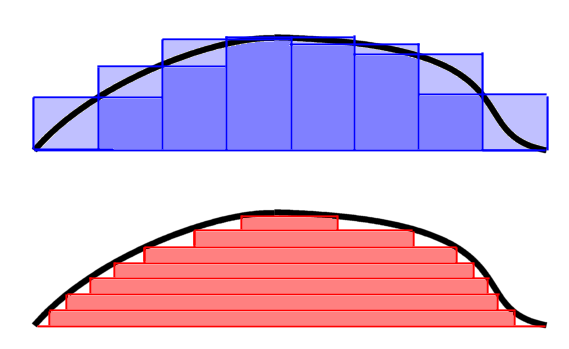
\includegraphics[width=0.5\textwidth]{fig_int_8}
	\caption{Riemann (top) versus Lebesgue integration (bottom).}
	\label{fig_int_8}
	\end{center}
\end{figure}


\end{remark}
\fi

\section{The fundamental theorem of calculus}\label{sec:FTC}

\subsection{Mean value theorem for definite integrals}
\ifcourse
	\checkoddpage
\marginpar{\ifoddpage\hspace*{-1.5cm}\else\hspace*{0.25cm}\fi
\includegraphics[width=0.075\textwidth]{youtube}\\
\ifoddpage\hspace*{-1.75cm}\else\hspace*{0.1cm}\fi
\qrcode[height=1.75cm]{https://youtu.be/59UeshgSuEE}
%\includegraphics[width=0.1\textwidth]{mvt_int}
}
 \fi
Consider the graph of a function $f$ in Figure \ref{fig_int_9a} and the area defined by $\int_1^4 f(x)\ dx$. In Figure~\ref{fig_int_9b}, the height of the rectangle is greater than $f$ on $[1,4]$, hence the area of this rectangle is greater than $\int_1^4 f(x)\ dx$. In Figure~\ref{fig_int_9c}, the height of the rectangle is smaller than $f$ on $[1,4]$, hence the area of this rectangle is less than $\int_1^4 f(x)\ dx$. Finally, in Figure~\ref{fig_int_9d} the height of the rectangle is such that the area of the rectangle is exactly that of $\int_1^4 f(x)\ dx$. Since rectangles that are too big, as in Figure~\ref{fig_int_9b}, and rectangles that are too little, as in Figure~\ref{fig_int_9c}, give areas greater/lesser than $\int_1^4 f(x)\ dx$, it makes sense that there is a rectangle, whose top intersects $f(x)$ somewhere on $[1,4]$, whose area is exactly that of the definite integral.


\begin{figure}[h]
\centering
%\raisebox{0.5cm}{
\subfigure[\label{fig_int_9a}]{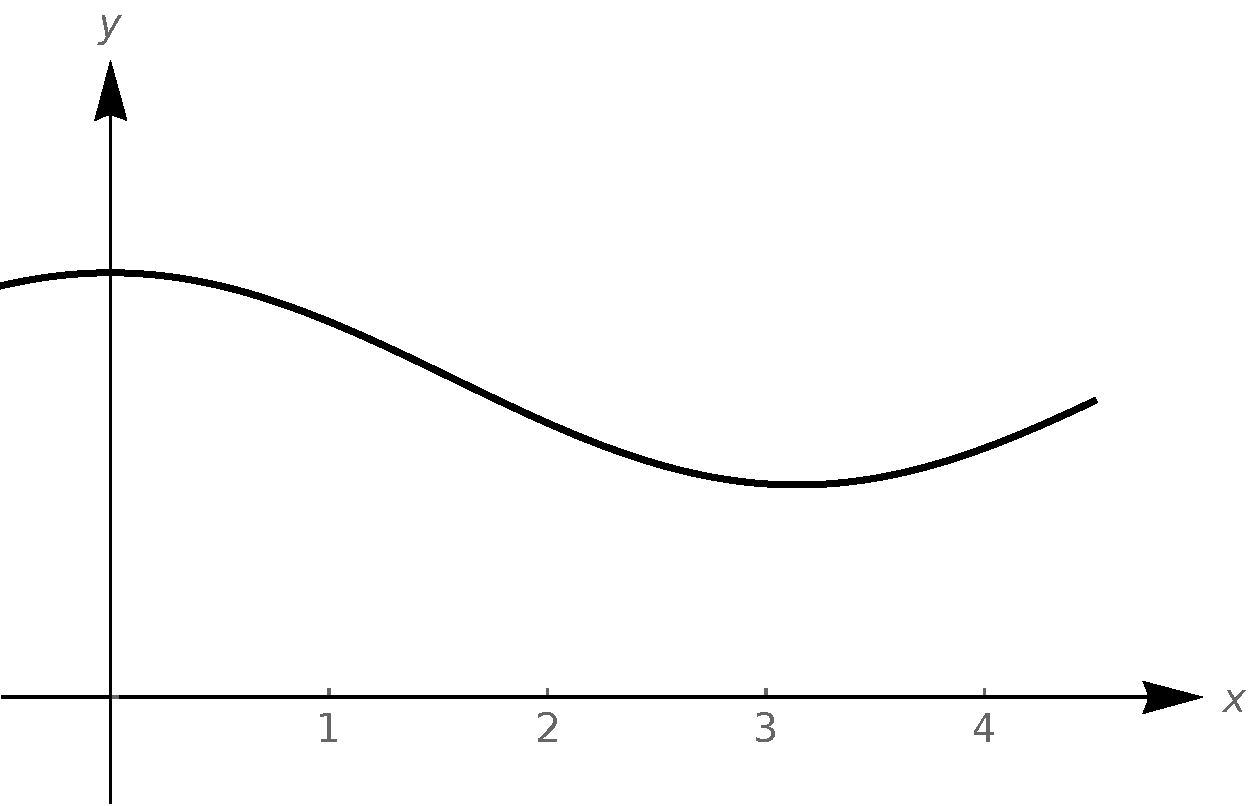
\includegraphics[width=0.3\textwidth]{fig_int_9a}}
\qquad
\subfigure[\label{fig_int_9b}]{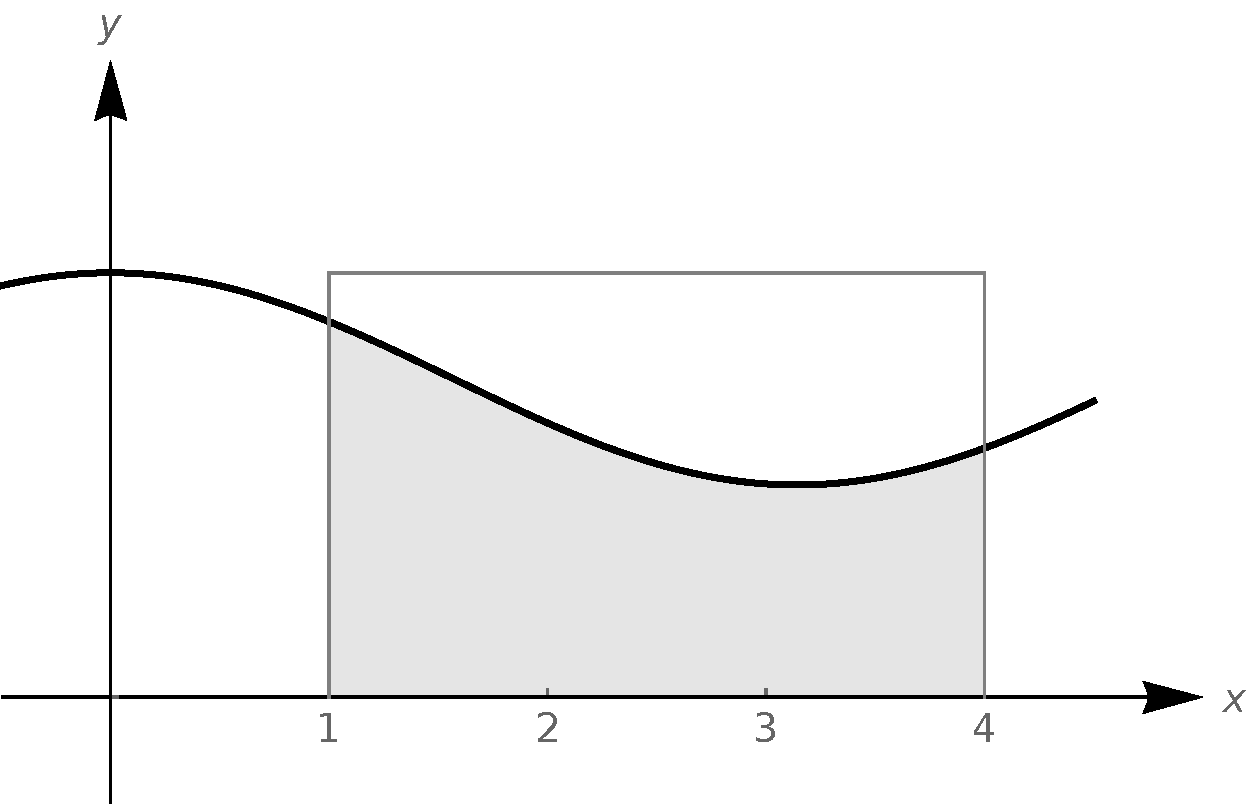
\includegraphics[width=0.3\textwidth]{fig_int_9b} }\\
\subfigure[\label{fig_int_9c}]{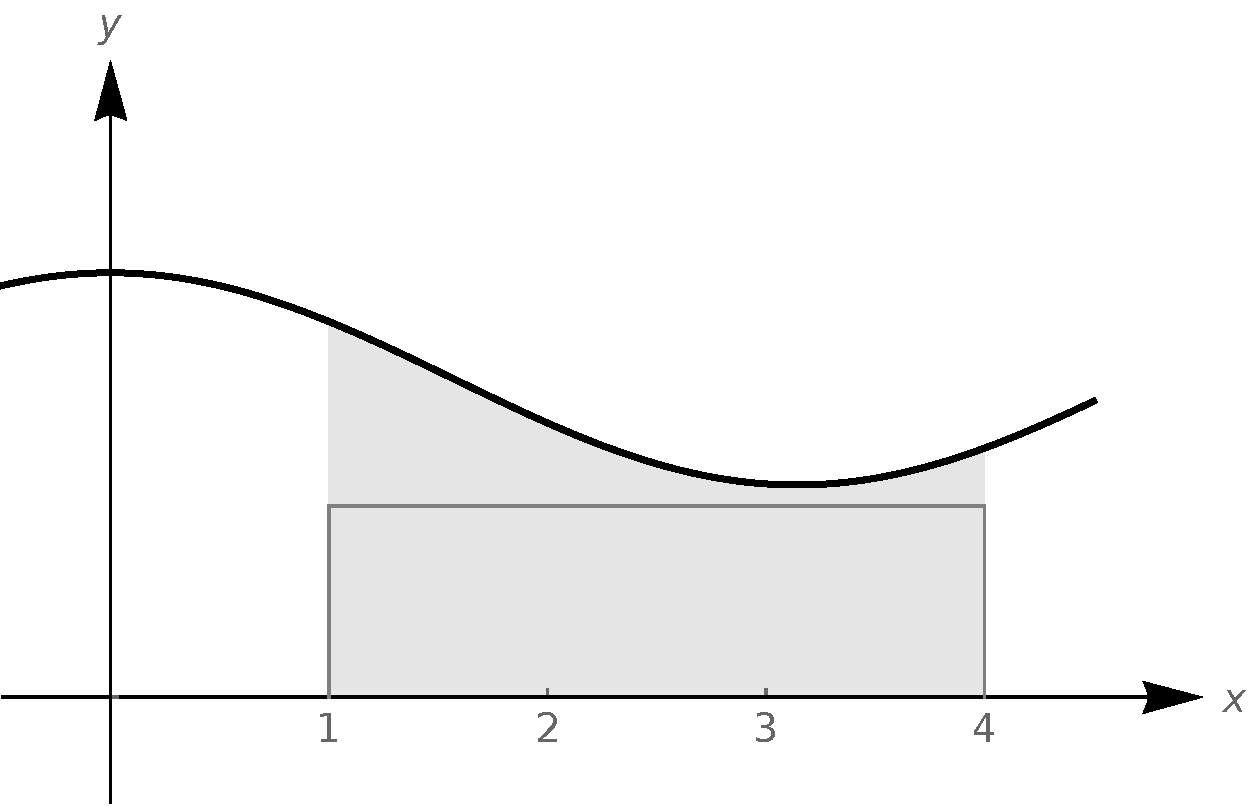
\includegraphics[width=0.3\textwidth]{fig_int_9c} }
\qquad
\subfigure[\label{fig_int_9d}]{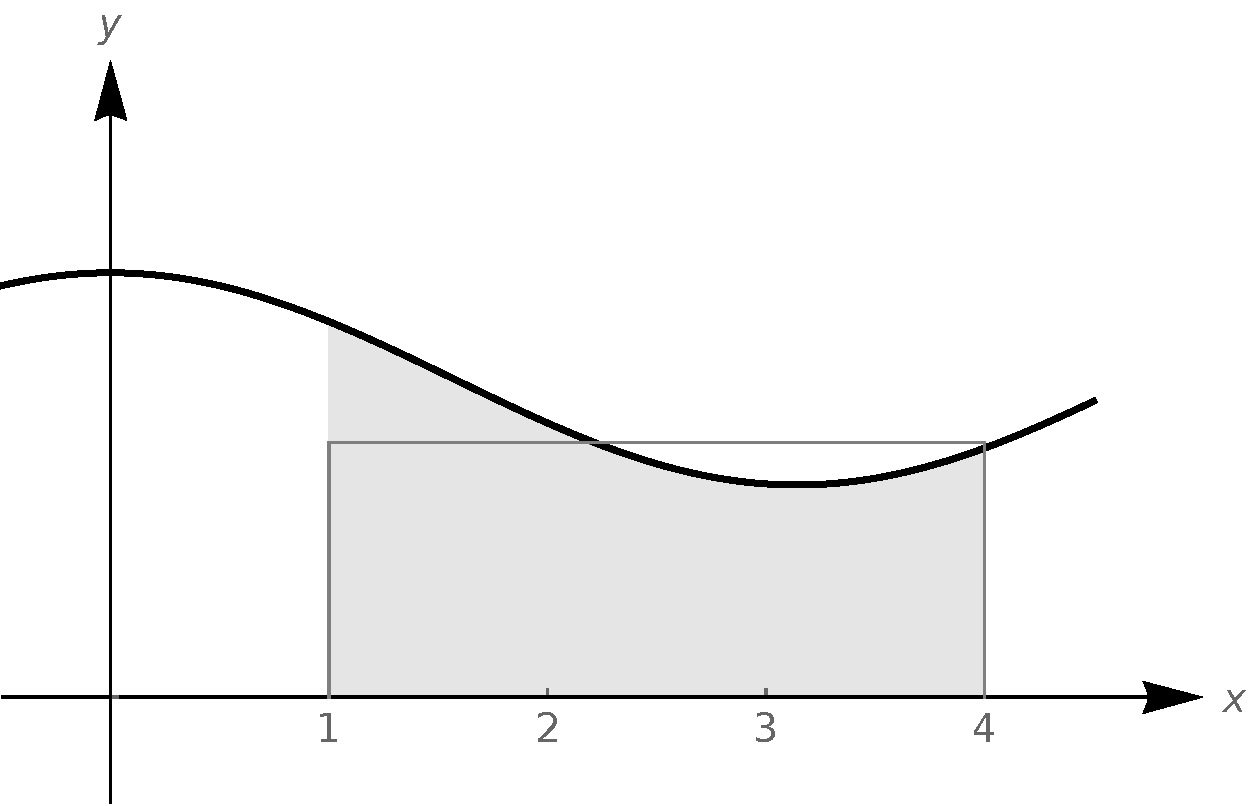
\includegraphics[width=0.3\textwidth]{fig_int_9d} }
\caption{The graph of a function $f$ (a) and differently sized rectangles give upper and lower bounds on $\int_1^4 f(x)\ dx$ (b-c).}
\end{figure} 


We state this idea formally in a theorem.

\begin{theorem}[The mean value theorem of integration]\label{thm:mvt2}
Let $f$ be continuous on $[a,b]$.\index{mean value theorem of integration}\index{integration! mean value theorem} There exists a value $c$ in $]a,b[$ such that $$\ds \int\limits_a^bf(x)\ dx = f(c)(b-a).$$
\end{theorem}
\index[aut]{middelwaardestelling}

This is an existential statement; $c$ exists, but we do not provide a method of finding it. Theorem \ref{thm:mvt2} is directly connected to the mean value theorem of differentiation (Theorem \ref{thm:mvt}).

\ifanalysis

\begin{proof}
Let us prove this theorem by considering a more general formulation. Namely, if  $f : [a, b] \to\mathbb{R}$ is continuous and $g$ is an integrable function that does not change sign on $[a, b]$, then there exists $c$ in $\left.\right]a, b\left[\right.$ such that
\begin{equation}
\ds \int\limits _{a}^{b}f(x)g(x)\,dx=f(c)\ds \int\limits _{a}^{b}g(x)\,dx.
\label{mvt_gen}
\end{equation}
Clearly, we obtain the expression used in Theorem~\ref{thm:mvt2} by letting $g(x)=1$. 

Now to prove Equation~\eqref{mvt_gen}. Let us assume that $f : [a, b] \to\mathbb{R}$ is continuous and $g$ is a nonnegative integrable function on $[a, b]$. By the extreme value theorem (Theorem~\ref{thm:extreme_val}), there exists $m$ and $M$ such that for each $x$ in $[a, b]$, it holds that $m\leq f(x)\leq M $ and $\displaystyle f[a,b]=[m,M]$. Since $g$ is nonnegative, we may write that
$$
\displaystyle m\ds \int\limits _{a}^{b}g(x)\,dx\leqslant \ds \int\limits _{a}^{b}f(x)g(x)\,dx\leqslant M\ds \int\limits _{a}^{b}g(x)\,dx.
$$

Now let
$$
\displaystyle I=\ds \int\limits _{a}^{b}g(x)\,dx.
$$

Obviously, if $I=0$, we are done since
$$
\displaystyle 0\leqslant \ds \int\limits _{a}^{b}f(x)g(x)\,dx\leqslant 0
$$
means
$$
\displaystyle \ds \int\limits _{a}^{b}f(x)g(x)\,dx=0,
$$

so for any $c$ in $\left.\right]a, b\left[\right.$,
$$
\ds \int\limits _{a}^{b}f(x)g(x)\,dx=f(c)I=0.
$$
If $I \neq 0$, then
$$
\displaystyle m\leqslant {\frac {1}{I}}\ds \int\limits _{a}^{b}f(x)g(x)\,dx\leqslant M.
$$
By the intermediate value theorem, $f$ attains every value of the interval $[m, M]$, so for some  $c$ in $\left.\right]a, b\left[\right.$ we have
$$
\displaystyle f(c)={\frac {1}{I}}\ds \int\limits _{a}^{b}f(x)g(x)\,dx,
$$
that is,
$$
\displaystyle \ds \int\limits _{a}^{b}f(x)g(x)\,dx=f(c)\ds \int\limits _{a}^{b}g(x)\,dx.
$$

Finally, if $g$ is negative on $[a, b]$, then
$$
\displaystyle M\ds \int\limits _{a}^{b}g(x)\,dx\leqslant \ds \int\limits _{a}^{b}f(x)g(x)\,dx\leqslant m\ds \int\limits _{a}^{b}g(x)\,dx,
$$
and we still get the same result as above. 
\end{proof}

\fi
\subsection{Main theorems}
Let $f(t)$ be a continuous function defined on $[a,b]$. The definite integral $\int_a^b f(x)\ dx$ is the area under $f\ $ on $[a,b]$. We can turn this concept into a function by letting the upper (or lower) bound vary.

Let $F(x) = \int_a^x f(t)\ dt$. It computes the area under $f$ on $[a,x]$ as illustrated in Figure \ref{fig_int_10}. We can study this function using our knowledge of the definite integral.  %If $f(t)>0$, then $F(x)>0$ when $x>a$ (consider the figure for a visual understanding). If $f$ is defined for values less than $a

\begin{figure}[h]
	\begin{center}
			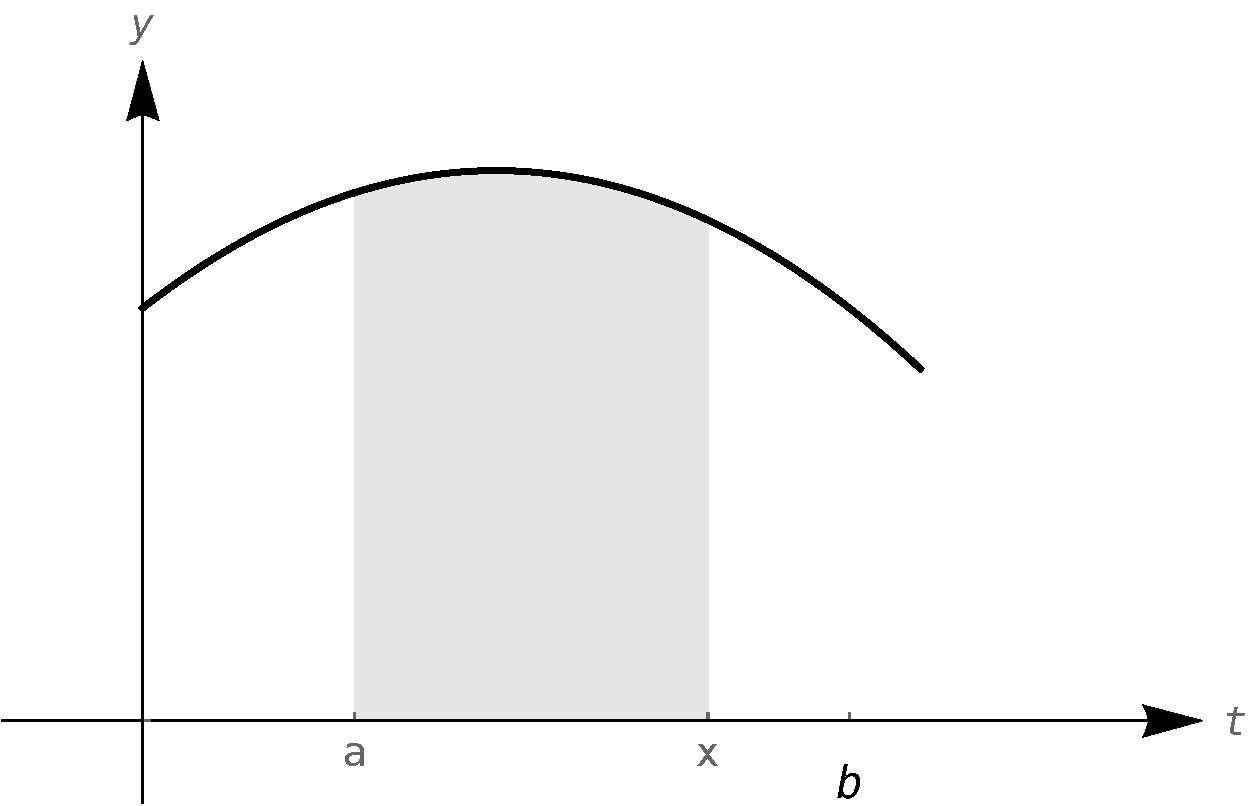
\includegraphics[width=0.5\textwidth]{fig_int_10}
	\caption{The area of the shaded region is $F(x) = \int_a^x f(t)\ dt$.}
	\label{fig_int_10}
	\end{center}
\end{figure}


We can also apply calculus ideas to $F(x)$; in particular, we can compute its derivative. While this may seem like an innocuous thing to do, it has far--reaching implications, as demonstrated by the fact that the result is given as an important theorem.




\pagebreak
\begin{theorem}[The fundamental theorem of calculus, Part 1]\label{thm:FTC1}
Let $f$ be continuous on $[a,b]$ and let $F(x) =  \int_a^x f(t)\ dt$. Then $F$ is a differentiable function on $]a,b[$, and\index{Fundamental Theorem of Calculus}\index{integration!Fun. Thm. of Calc.} $$\Fp(x)=f(x).$$
\end{theorem}
\index[aut]{Hoofdstelling van de integraalrekening}

\ifanalysis

\begin{proof}
For a given $f(t)$, let us define the function $F(x)$ as
$$
\displaystyle F(x)=\ds \int\limits_{a}^{x}f(t)\,dt.
$$
For any two numbers $x_1$ and $x_1 + \Delta x$ in $[a, b]$, we have
$$
\displaystyle F(x_{1})=\ds \int\limits _{a}^{x_{1}}f(t)\,dt
$$
and likewise
$$
\displaystyle F(x_{1}+\Delta x)=\ds \int\limits _{a}^{x_{1}+\Delta x}f(t)\,dt.
$$
Subtracting these two equalities yields
\begin{equation}
\displaystyle F(x_{1}+\Delta x)-F(x_{1})=\ds \int\limits_{a}^{x_{1}+\Delta x}f(t)\,dt-\ds \int\limits _{a}^{x_{1}}f(t)\,dt.
\label{hoofd_int_1}
\end{equation}
Using Theorem~\ref{thm:defintprop} we can rewrite the right hand side of Equation~\eqref{hoofd_int_1} as
$$
\ds \int\limits _{a}^{x_{1}+\Delta x}f(t)\,dt-\ds \int\limits _{a}^{x_{1}}f(t)\,dt=\int\limits _{a}^{x_{1}+\Delta x}f(t)\,dt+\ds \int\limits _{x_1}^{a}f(t)\,dt=\ds \int\limits _{x_{1}}^{x_{1}+\Delta x}f(t)\,dt.
$$
Hence, Equation~\eqref{hoofd_int_1} becomes
\begin{equation}
\displaystyle F(x_{1}+\Delta x)-F(x_{1})=\ds \int\limits _{x_{1}}^{x_{1}+\Delta x}f(t)\,dt.
\label{hoofd_int_2}
\end{equation}
According to the mean value theorem for integration (Theorem~\ref{thm:mvt2}), there exists a real number $\displaystyle c\in [x_{1},x_{1}+\Delta x]$ such that
$$
\ds \int\limits _{x_{1}}^{x_{1}+\Delta x}f(t)\,dt=f(c)\cdot \Delta x.
$$
This expression allows us to rewrite Equation~\eqref{hoofd_int_2} as 
\begin{equation}
\displaystyle F(x_{1}+\Delta x)-F(x_{1})=f(c)\cdot \Delta x.
\label{hoofd_int_3}
\end{equation}
Note that we just write $c$ in order not to overload the notation, but one should keep in mind that, for a given function $f$,  the value of $c$ depends on $x_1$  and on $\Delta x$, though it is always confined to the interval $\,[x_{1},x_{1}+\Delta x]$.

Now, dividing both sides of Equation~\eqref{hoofd_int_3} by $\Delta x$ gives
$$
\displaystyle {\frac {F(x_{1}+\Delta x)-F(x_{1})}{\Delta x}}=f(c),
$$
whose left side is the difference quotient for $F$ at $x_1$. So, let us take the limit as $\displaystyle \Delta x\to0$  on both sides of the equation. This yields: 
\begin{equation}
\displaystyle \lim _{\Delta x\to 0}{\frac {F(x_{1}+\Delta x)-F(x_{1})}{\Delta x}}=\lim _{\Delta x\to 0}f(c).
\label{hoofd_int_4}
\end{equation}
Clearly, the expression on the left side of the resulting equation is the definition of the derivative of $F$ at $x_1$, so we may rewrite Equation~\eqref{hoofd_int_4} as
\begin{equation}
\displaystyle F'(x_{1})=\lim _{\Delta x\to 0}f(c).
\label{hoofd_int_5}
\end{equation}

To find the limit on the right side of Equation~\eqref{hoofd_int_5}, we resort to the squeeze theorem (Theorem~\ref{thm:sqz}). The number $c$ is in the interval $[x_1, x_1 + \Delta x]$, so $x_1 \leq c \leq x_1 + \Delta x$. Besides, it holds that 
$$
\displaystyle \lim _{\Delta x\to 0}x_{1}=x_{1}
$$
and 
$$
\displaystyle \lim _{\Delta x\to 0}\left(x_{1}+\Delta x\right)=x_{1}.
$$
Therefore, according to the squeeze theorem, it must hold that
$$
\displaystyle \lim _{\Delta x\to 0}c=x_{1}.
$$
Consequently, we may rewrite  Equation~\eqref{hoofd_int_5} as
$$
\displaystyle F'(x_{1})=\lim _{c\to x_{1}}f(c).
$$

The function $f$ is continuous at $c$, so the limit can be taken inside the function. In this way, we get
$$
\displaystyle F'(x_{1})=f(x_{1}),
$$
which completes the proof.
\end{proof}

\fi

To illustrate this theorem, let us consider
$$\ds F(x) = \ds \int\limits_{-5}^x (t^2+\sin (t))\ dt$$
and try to find $\Fp(x)$. 

Using Theorem~\ref{thm:FTC1}, we immediately have $\Fp(x) = x^2+\sin (x)$.  This simple example reveals that $F(x)$ is an antiderivative of $x^2+\sin (x)$! Therefore, $F(x) = x^3/3-\cos (x)+C$ for some value of $C$.  We have done more, however, than found a complicated way of computing an antiderivative. Consider a function $f$ defined on an open interval containing $a$, $b$ and $c$. Suppose we want to compute $\int_a^b f(t)\ dt$. First, let 
$$F(x) = \int_c^x f(t)\ dt.$$
Using the properties of the definite integral (Theorem \ref{thm:defintprop}), we know 
		\begin{align*}\ds \int\limits_a^b f(t)\ dt &= \ds \int\limits_a^c f(t)\ dt + \ds \int\limits_c^b f(t)\ dt \\[0.2cm]
											&= -\ds \int\limits_c^a f(t)\ dt + \ds \int\limits_c^b f(t)\ dt \\[0.2cm]
											&=-F(a) + F(b)\\[0.2cm]
											&= F(b) - F(a).
		\end{align*}
We now see how indefinite integrals and definite integrals are related: we can evaluate a definite integral using antiderivatives.  This is the second part of the fundamental theorem of calculus.

\begin{theorem}[The fundamental theorem of calculus, Part 2]\label{thm:FTC2}
Let $f$ be continuous on $[a,b]$ and let $F$ be \textit{any} antiderivative of $f$. Then\index{dundamental theorem of calculus}$$\ds \int\limits_a^b f(x)\ dx = F(b) - F(a).$$
\end{theorem}
\index[aut]{Hoofdstelling van de integraalrekening}

\ifanalysis

\begin{proof}
We will rely on Riemann sums to prove this theorem in a more rigorous way. For that purpose, let $f$ be integrable on the interval $[a, b]$, and let $f$ admit an antiderivative $F$ on $[a, b]$. Consider the quantity $F(b) - F(a)$ and let there be a partition of size $\mathcal{L}$ with numbers $x_1, x_2, \ldots, x_{n+1}$ such that
$$
\displaystyle a=x_{1}<x_{2}<\cdots <x_{n}<x_{n+1}=b.
$$
Clearly, 
$$
\displaystyle F(b)-F(a)=F(x_{n+1})-F(x_{1}).
$$
Now, for $i=2,\ldots, n$ we add each $F(x_i)$ along with its additive inverse, so that the resulting quantity is equal:
$$
\displaystyle {\begin{aligned}F(b)-F(a)&=F(x_{n+1})+[-F(x_{n})+F(x_{n})]+\cdots +[-F(x_{2})+F(x_{2})]-F(x_{1})\\&=[F(x_{n+1})-F(x_{n})]+[F(x_{n})-F(x_{n-1})]+\cdots +[F(x_{3})-F(x_{2})]+[F(x_{2})-F(x_{1})].\end{aligned}}
$$
Or shorter: 
\begin{equation}
\displaystyle F(b)-F(a)=\sum _{i=1}^{n}\,[F(x_{i+1})-F(x_{i})].
\label{hoofd_int_6}
\end{equation}
Inspecting the right hand side of this equation reminds us to the mean value theorem of differentiation (Theorem~\ref{thm:mvt}). Indeed, it tells us that 
$$
\displaystyle F'(c)={\frac {F(b)-F(a)}{b-a}},
$$
where $c\in[a,b]$, or equivalently
$$
\displaystyle F(b)-F(a)=F'(c)(b-a).
$$
Hence, since the function $F$ is differentiable on the interval $[a, b]$ and hence differentiable and continuous on each interval $[x_{i-1}, x_i]$, we can rewrite the terms appearing in right hand side of Equation~\eqref{hoofd_int_6} as
$$
\displaystyle F(x_{i+1})-F(x_{i})=F'(c_{i})(x_{i+1}-x_{i})\,,
$$
where $c_i\in[x_{i+1},x_i]$. 
This allows us to rewrite Equation~\eqref{hoofd_int_6} as
$$
\displaystyle F(b)-F(a)=\sum _{i=1}^{n}\,[F'(c_{i})(x_{i+1}-x_{i})].
$$
Moreover, our assumption that $F$ is an antiderivative of $f$ implies  that $F'(c_{i})=f(c_{i})$. Hence, letting $x_{i+1}-x_{i}= \Delta x_i$, we get 
\begin{equation}
\displaystyle F(b)-F(a)=\sum _{i=1}^{n}\,[f(c_{i})(\Delta x_{i})].
\label{hoofd_int_7}
\end{equation}
Essentially, we are describing with this expression the area of a rectangle, with the width times the height, and we are adding the areas together. By taking the limit of the expression as the norm of the partitions approaches zero, we arrive at the Riemann integral. We know that this limit exists because $f$ was assumed to be integrable. So, we take the limit on both sides of Equation~\eqref{hoofd_int_7}, to obtain
$$
\displaystyle \lim _{\mathcal{L}\to 0}\left(F(b)-F(a)\right)=\lim _{\mathcal{L}\to 0}\sum _{i=1}^{n}\,[f(c_{i})(\Delta x_{i})].
$$
Neither $F(b)$ nor $F(a)$ is dependent on $\displaystyle \mathcal{L}$, so the limit on the left side remains $F(b) - F(a)$. Furthermore, the expression on the right side of the equation defines the integral over $f$ from $a$ to $b$ (Theorem~\ref{thm:riemann_sum}). Therefore, we obtain
$$
\displaystyle F(b)-F(a)=\ds \int\limits _{a}^{b}f(x)\,dx,
$$
which completes the proof.
\end{proof}

\fi


\begin{example}\label{ex_ftc3}
We spent a great deal of time in the previous section studying $\int_0^4(4x-x^2)\ dx$. Using the fundamental theorem of calculus, evaluate this definite integral. 


\xhrulefill{gray}{2.5pt}Solution \xhrulefill{gray}{2.5pt}

We need an antiderivative of $f(x)=4x-x^2$. All antiderivatives of $f$ have the form $$F(x) = 2x^2-\frac13x^3+C\,;$$ for simplicity, choose $C=0$.

The fundamental theorem of calculus states 
		$$\ds \int\limits_0^4(4x-x^2)\ dx = F(4)-F(0) = \left(2(4)^2-\frac134^3-\big(0-0\big)\right) = 32-\frac{64}3 = \dfrac{32}{3}.$$
This is the same answer we obtained using limits in the previous section, just with much less work.
\end{example}

A special notation is often used in the process of evaluating definite integrals using the fundamental theorem of calculus. Instead of explicitly writing $F(b)-F(a)$, the notation $F(x)\Big|_a^b$ is used. Also note that  any antiderivative $F(x)$ can be chosen when using the fundamental theorem of calculus to evaluate a definite integral, meaning any value of $C$ can be picked. The constant always cancels out of the expression when evaluating $F(b)-F(a)$, so it does not matter what value is picked. This being the case, we might as well let $C=0$.

\begin{example}\label{ex_ftc4}
Evaluate the following definite integrals.
\begin{multicols}{5}
\begin{enumerate}
\item	$\ds \int\limits_{-2}^2 x^3\ dx $
\item	$\ds \int\limits_0^\pi \sin (x)\ dx $ 
\item	$\ds \int\limits_0^5e^t\ dt$
\item	$\ds \int\limits_4^9 \sqrt{u}\ du $
\item	$\ds \int\limits_1^5 2\ dx $ 
\end{enumerate}
\end{multicols}



\xhrulefill{gray}{2.5pt}Solution \xhrulefill{gray}{2.5pt}

\begin{enumerate}
\item	$\ds \int\limits_{-2}^2 x^3\ dx = \left.\frac14x^4\right|_{-2}^2 = \left(\frac142^4\right) - \left(\frac14(-2)^4\right) = 0.$
\item		$\ds \int\limits_0^\pi \sin (x)\ dx = -\cos (x)\Big|_0^\pi = -\cos (\pi)- \big(-\cos 0\big) = 1+1=2.$ So, the area under one hump of a sine curve is 2.
\item	 $\ds \int\limits_0^5e^t\ dt = e^t\Big|_0^5 = e^5 - e^0 = e^5-1 \approx 147.41.$
\item		$\ds \int\limits_4^9 \sqrt{u}\ du = \int_4^9 u^\frac12\ du = \left.\frac23u^\frac32\right|_4^9 = \frac23\left(9^\frac32-4^\frac32\right) = \frac23\big(27-8\big) =\frac{38}3.$
\item		$\ds \int\limits_1^5 2\ dx = 2x\Big|_1^5 = 2(5)-2=2(5-1)=8.$ 

\end{enumerate}
\end{example}
This last integral in Example~\ref{ex_ftc4} is interesting; the integrand is a constant function, hence we are finding the area of a rectangle with width $(5-1)=4$ and height 2. Notice how the evaluation of the definite integral led to $2(4)=8$. 

In general, if $c$ is a constant, then 
$$\ds \int\limits_a^b c\ dx = c(b-a).$$

\subsection{Motion and the fundamental theorem of calculus}

We established, starting in Section \ref{sec:interp_deriv}, that the derivative of a position function is a velocity function, and the derivative of a velocity function is an acceleration function. Now consider definite integrals of velocity and acceleration functions. Specifically, if $v(t)$ is a velocity function, what does $ \int_a^b v(t)\ dt$ mean?\index{integration ! displacement}\index{displacement}

The fundamental theorem of calculus states that
$$\ds \int\limits_a^b v(t)\ dt = V(b) - V(a),$$ 
where $V(t)$ is any antiderivative of $v(t)$. Since $v(t)$ is a velocity function, $V(t)$ must be a position function, and $V(b) - V(a)$ measures a change in position, or \textbf{displacement} (\textit{verplaatsing}).

\begin{example}\label{ex_ftcmotion1}
A ball is thrown straight up with velocity given by $v(t) = -32t+20$m/s, where $t$ is measured in seconds. Find, and interpret, $\int_0^1 v(t)\ dt.$

\ifanalysis\pagebreak\fi
\xhrulefill{gray}{2.5pt}Solution \xhrulefill{gray}{2.5pt}

Using the fundamental theorem of calculus, we have 
\allowdisplaybreaks
\begin{align*}
\ds \int\limits_0^1 v(t)\ dt &= \ds \int\limits_0^1 (-32t+20)\ dt \\[0.2cm]
			&= -16t^2 + 20t\Big|_0^1 \\[0.2cm]
			&= 4.
\end{align*}
Thus if a ball is thrown straight up into the air with velocity $v(t) = -32t+20$, the height of the ball, 1 second later, will be 4 metres above the initial height. 
\end{example}


Integrating a rate of change function gives total change. Velocity is the rate of position change; integrating velocity gives the total change of position, i.e., displacement.

Integrating a speed function gives a similar, though different, result. Speed is also the rate of position change, but does not account for direction. So integrating a speed function gives total change of position, without the possibility of negative position change. Hence the integral of a speed function gives \textbf{distance travelled} (\textit{afgelegde afstand}).

\subsection{The fundamental theorem of calculus and the chain rule}
Using other notation, we may write Part 1 of the fundamental theorem of calculus as
$$\ds \frac{d}{dx}\big(F(x)\big) = f(x).$$
While we have just practised evaluating definite integrals, sometimes finding antiderivatives is impossible and we need to rely on other techniques to approximate the value of a definite integral. Functions written as 
$$F(x) = \ds \int\limits_a^x f(t)\ dt$$
 are useful in such situations.

It may be of further use to compose such a function with another. As an example, we may compose $F(x)$ with $g(x)$ to get $$F\big(g(x)\big) = \ds \int\limits_a^{g(x)} f(t)\ dt.$$ What is the derivative of such a function? 
The chain rule can be employed to find $$\frac{d}{dx}\Big(F\big(g(x)\big)\Big) = \Fp\big(g(x)\big)g'(x) = f\big(g(x)\big)g'(x).$$

An example will help us understand this.


\begin{example}\label{ex_ftc11}
Find the derivative of 
\begin{multicols}{2}
\begin{enumerate}
    \item $\ds F(x) = \ds \int\limits_2^{x^2} \ln (t)\ dt$
    \item $\ds F(x) = \ds \int\limits_{\cos (x)}^5 t^3\ dt.$
\end{enumerate}
\end{multicols}

\ifcalculus\pagebreak\fi
\xhrulefill{gray}{2.5pt}Solution \xhrulefill{gray}{2.5pt}

\begin{enumerate}
\item We can view $F(x)$ as being the function $ G(x) = \int_2^x \ln(t)\ dt$ composed with $h(x) = x^2$; that is, $F(x) = G\big(h(x)\big)$. The fundamental theorem of calculus states that $G'(x) = \ln (x)$. The chain rule gives us 
\begin{align*}
F'(x) &= G'\big(h(x)\big) h'(x) \\
 			&= \ln (h(x)) h'(x) \\
 			&= \ln (x^2) 2x \\
 			&=2x\ln (x^2).
\end{align*}
Normally, of course, the steps defining $G(x)$ and $h(x)$ are skipped.
\item Note that $ F(x) = -\int_5^{\cos (x)} t^3\ dt$. Viewed this way, the derivative of $F$ is straightforward:
$$F'(x) = \sin (x) \cos^3 (x).$$
\end{enumerate}
\end{example}
%
%\subsection{Area between curves}
%Consider continuous functions $f(x)$ and $g(x)$ defined on $[a,b]$, where $f(x) \geq g(x)$ for all $x$ in $[a,b]$, as demonstrated in Figure \ref{fig_int_9}. What is the area of the shaded region bounded by the two curves over $[a,b]$?
%
%
%The area can be found by recognizing that this area is the area under $f$ minus the area under $g$. Using mathematical notation, the area is 
%$$\ds \int\limits_a^b f(x)\ dx - \ds \int\limits_a^b g(x)\ dx.$$ Properties of the definite integral allow us to simplify this expression to $$ \ds \int\limits_a^b\big(f(x) - g(x)\big)\ dx.$$
%
%\begin{figure}[h]
%	\begin{center}
%			\includegraphics[width=0.5\textwidth]{fig_int_9}
%	\caption{Finding the area bounded by two functions on an interval.}
%	\label{fig_int_9}
%	\end{center}
%\end{figure}
%
%\begin{example}\label{ex_ftc6}
%Find the area of the region enclosed by $y=x^2+x-5$ and $y=3x-2$.
%
%\xhrulefill{gray}{2.5pt}Solution \xhrulefill{gray}{2.5pt}
%
%It will help to sketch these two functions, as done in Figure \ref{fig_int_10}. The region whose area we seek is completely bounded by these two functions; they seem to intersect at $x=-1$ and $x=3$. To check, set $x^2+x-5=3x-2$ and solve for $x$:
%\[ 
%\begin{array}{rrclr}
%&x^2+x-5 & = & 3x-2 & \\
%\Leftrightarrow&(x^2+x-5) - (3x-2) & = &  0 \\
%\Leftrightarrow&x^2-2x-3 & = & 0 &\\
%\Leftrightarrow&(x-3)(x+1) & = & 0 &\\
%\Leftrightarrow& x = -1 & \vee &x=3\,.&\\
%\end{array} \]
%
%Consequently, the area we are seeking is 
%	\begin{align*}\ds \int\limits_{-1}^3\big(3x-2 -(x^2+x-5)\big)\ dx &= \ds \int\limits_{-1}^3 (-x^2+2x+3)\ dx \\[0.2cm]
%							&=\left.\left(-\frac13x^3+x^2+3x\right)\right|_{-1}^3 \\[0.2cm]
%							&=-\frac13(27)+9+9-\left(\frac13+1-3\right)= 9+\frac{5}{3}\\[0.2cm]
%							& = \frac{32}{3} \approx 10.67.
%	\end{align*}
%	\begin{figure}[H]
%	\begin{center}
%			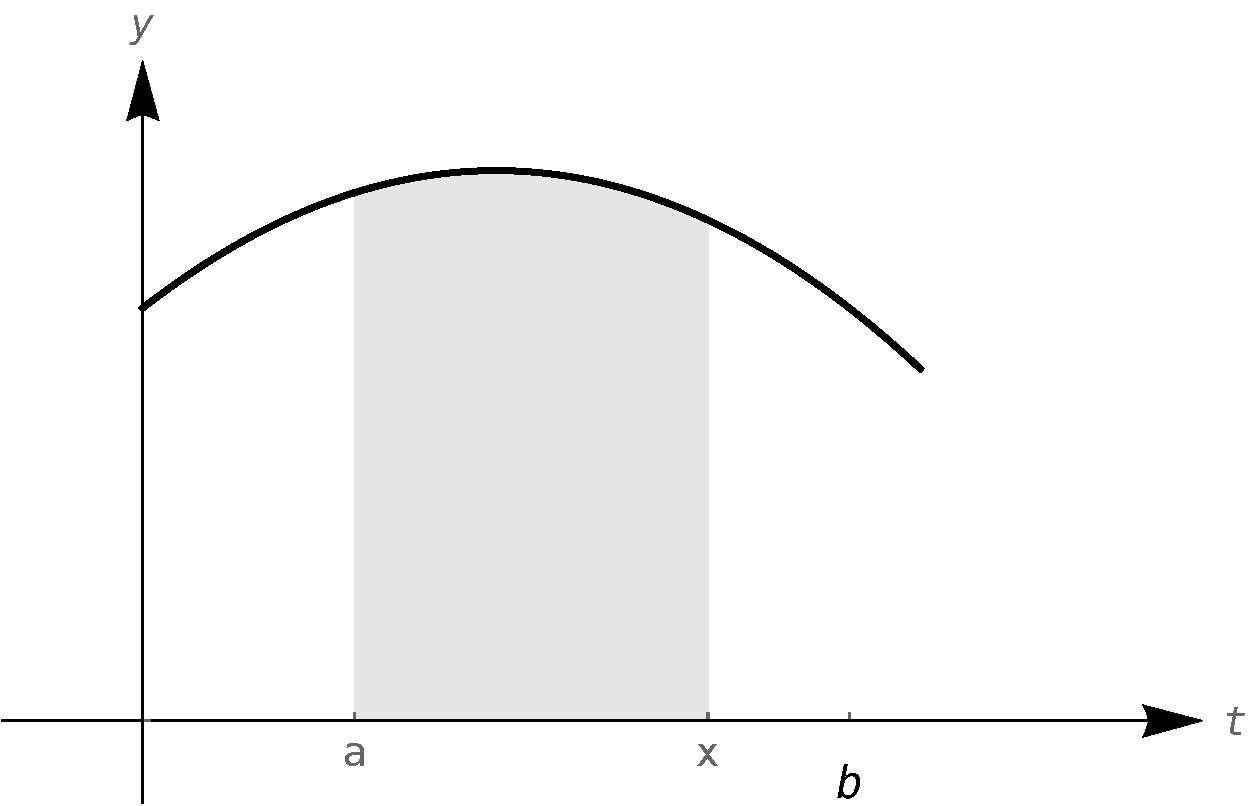
\includegraphics[width=0.46\textwidth]{fig_int_10}
%	\caption{Sketching the region enclosed by $y=x^2+x-5$ and $y=3x-2$ in Example \ref{ex_ftc6}.}
%	\label{fig_int_10}
%	\end{center}
%\end{figure}
%\vspace*{-1cm}
%\end{example}

\subsection{Average value}
\ifcourse
	\checkoddpage
\marginpar{\ifoddpage\hspace*{-1.5cm}\else\hspace*{0.25cm}\fi
\includegraphics[width=0.075\textwidth]{youtube}\\
\ifoddpage\hspace*{-1.75cm}\else\hspace*{0.1cm}\fi
\qrcode[height=1.75cm]{https://youtu.be/NCF4m8BDs7w}
%\includegraphics[width=0.1\textwidth]{mean_function_value}
}
 \fi
Recognize that the mean value theorem can be rewritten as 
$$f(c) = \frac{1}{b-a}\ds \int\limits_a^b f(x)\ dx,$$
 for some value of $c$ in $[a,b]$. Next, partition the interval $[a,b]$ into $n$ equally spaced subintervals, $a=x_1 < x_2 < \ldots < x_{n+1}=b$ and choose any $c_i$ in $[x_i,x_{i+1}]$. The average of the numbers $f(c_1)$, $f(c_2)$, \ldots, $f(c_n)$ is:
	$$\dfrac{1}{n}\Big(f(c_1) + f(c_2) + \ldots + f(c_n)\Big) = \dfrac{1}{n}\sum_{i=1}^n f(c_i).$$ Multiply this last expression by 1 in the form of $\frac{(b-a)}{(b-a)}$:
	\begin{align*}
	\dfrac{1}{n}\sum_{i=1}^n f(c_i) &= \sum_{i=1}^n f(c_i)\dfrac{1}{n} \frac{(b-a)}{(b-a)} \\[0.2cm]
									&= \frac{1}{b-a} \sum_{i=1}^n f(c_i)\frac{b-a}n  \\[0.2cm]
									&=\frac{1}{b-a} \sum_{i=1}^n f(c_i)\Delta x\quad  % \\[0.2cm]
	\end{align*}
where $\Delta x = (b-a)/n$. Now take the limit as $n\to+\infty$:
		$$\lim_{n\to+\infty} \frac{1}{b-a} \ds\sum_{i=1}^n f(c_i)\Delta x =  \frac{1}{b-a} \ds \int\limits_a^b f(x)\ dx =   f(c).$$
This tells us this: when we evaluate $f$ at $n$ (somewhat) equally spaced points in $[a,b]$, the average value of these samples is $f(c)$ as $n\to+\infty$.

This leads us to a definition.

\begin{definition}[The average value of \textit{f} on \textit{[a,b]}] \label{def:av_val}
Let $f$ be continuous on $[a,b]$. The \textbf{average value of $f$} (\textit{gemiddelde functiewaarde}) on $[a,b]$ is $f(c)$, where $c$ is a value in $[a,b]$ guaranteed by the mean value theorem.\index{integration!average value}\index{average value of function}\index[aut]{integratie!gemiddelde}\index{functie!gemiddelde} I.e., 
$$\text{Average Value of $f$ on $[a,b]$} = \frac{1}{b-a}\int\limits_a^bf(x)\ dx.$$

\end{definition}

An application of this definition is given in the following example.\\

\enlargethispage{2\baselineskip}

\begin{example}\label{ex_ftc10}
An object moves back and forth along a straight line with a velocity given by $v(t) = (t-1)^2$ on $[0,3]$, where $t$ is measured in seconds and $v(t)$ is measured in m/s. 

\begin{enumerate}
\item What is the average velocity of the object?
\item What was the displacement of the object?
\end{enumerate}

\xhrulefill{gray}{2.5pt}Solution \xhrulefill{gray}{2.5pt}

\begin{enumerate}
\item By Definition~\ref{def:av_val}, the average velocity is:
	$$\frac{1}{3-0}\ds \int\limits_0^3 (t-1)^2\ dt =\frac13 \ds \int\limits_0^3 \big(t^2-2t+1\big)\ dt = \left.\frac13\left(\frac13t^3-t^2+t\right)\right|_0^3 = 1\text{ m/s}.$$
\item We calculate this by integrating its velocity function: $\int_0^3 (t-1)^2\ dt = 3$ m. Its final position was 3 meter from its initial position after 3 seconds: its average velocity was 1 m/s.
\end{enumerate}
\end{example}

This section has laid the groundwork for a lot of great mathematics to follow. The most important lesson is this: definite integrals can be evaluated using antiderivatives. Since the previous section established that definite integrals are the limit of Riemann sums, we can later create Riemann sums to approximate values other than area under the curve, convert the sums to definite integrals, then evaluate these using the fundamental theorem of calculus. This will allow us to compute the work done by a variable force, the volume of certain solids, the arc length of curves, and more.

The downside is this: generally speaking, computing antiderivatives is much more difficult than computing derivatives. For that reason, we will see in Section~\ref{pc:integratie}  how to approximate the value of definite integrals beyond using the left hand, right hand and midpoint rules. These techniques are invaluable when antiderivatives cannot be computed, or when the actual function $f$ is unknown and all we know is the value of $f$ at certain $x$-values. But first, we will study techniques of finding antiderivatives analytically so that a wide variety of definite integrals can be evaluated. 


%\section{Numerical Integration}\label{sec:numerical_integration}

\section{Techniques of antidifferentiation}\label{sec:techniques_of_antidifferentiation}
This chapter is devoted to exploring techniques of antidifferentiation. While not every function has an antiderivative in terms of elementary functions like polynomial, exponential or trigonometric functions, we can still find antiderivatives of a wide variety of functions. Nowadays there are also several websites that allow you to calculate integrals with steps\footnote{https://www.integral-calculator.com/}. 

\subsection{Substitution}\label{sec:substitution}
\subsubsection{Rationale}
\ifcourse
	\checkoddpage
\marginpar{\ifoddpage\hspace*{-1.5cm}\else\hspace*{0.25cm}\fi
\includegraphics[width=0.075\textwidth]{youtube}\\
\ifoddpage\hspace*{-1.75cm}\else\hspace*{0.1cm}\fi
\qrcode[height=1.75cm]{https://youtu.be/NCF4m8BDs7w}
%\includegraphics[width=0.1\textwidth]{substitutie}
}
\fi
Essentially, integration by \textbf{substitution} (\textit{substitutie}) allows us to undo the chain rule. Its underlying principle is to rewrite a complicated integral of the form $\int f(x)\ dx$ as a not--so--complicated integral $\int h(u)\ du$. 

For instance, consider
$$\int (20x+30)(x^2+3x-5)^9\ dx.$$
Arguably the most complicated part of the integrand is $(x^2+3x-5)^9$. We wish to make this simpler; we do so through a substitution. Let $u=x^2+3x-5$. Thus 
$$(x^2+3x-5)^9 = u^9.$$
We have established $u$ as a function of $x$, so now consider the differential of $u$: 
$$du = (2x+3)dx.$$ 

Let us return now to the original integral and do some substitutions through algebra:
\allowdisplaybreaks
\begin{align*}
	\int (20x+30)(x^2+3x-5)^9\ dx 	&=	\int 10(2x+3)(x^2+3x-5)^9\ dx \\
									&=\int 10(\underbrace{x^2+3x-5}_u)^9\underbrace{(2x+3)\ dx}_{du} \\
									&=\int 10u^9\ du \\
									&= u^{10} + C \quad\quad \text{ (Replace $u$ with $x^2+3x-5$.)}\\
									&= (x^2+3x-5)^{10} +C
\end{align*}

In general, let $F(x)$ and $g(x)$ be differentiable functions and consider the derivative of their composition: 
	$$\frac{d}{dx}\Big(F\big(g(x)\big)\Big) = \Fp(g(x))g'(x).$$ Thus 
	$$\int \Fp(g(x))g'(x)\ dx = F(g(x)) + C.$$
Integration by substitution works by recognizing the inside function $g(x)$ and replacing it with a variable. By setting $u=g(x)$, we can rewrite the derivative as
	$$\frac{d}{dx}\Big(F\big(u\big)\Big) = \Fp(u)u'.$$
Since $du = g'(x)dx$, we can rewrite the above integral as
	$$\int \Fp(g(x))g'(x)\ dx = \int \Fp(u) du = F(u)+C = F(g(x))+ C.$$


The point of substitution is to make the integration step easy. Indeed, the step $\int \Fp(u)\ du = F(u) + C$ looks easy, as the antiderivative of the derivative of $F$ is just $F$, plus a constant. The work involved is making the proper substitution. There is not a step--by--step process that one can memorize; rather, experience will be one's guide. To gain experience, we now embark on some examples.

\begin{example}
Evaluate the following indefinite integrals:
\begin{multicols}{3}
\begin{enumerate}
\item $\ds \int \frac{7}{-3x+1}\ dx$,
\item $\ds \int x\sin(x^2+5)\ dx$,
\item $\ds\int x\sqrt{x+3}\ dx$.
\end{enumerate}
\end{multicols}

\xhrulefill{gray}{2.5pt}Solution \xhrulefill{gray}{2.5pt}

\begin{enumerate}
\item View the integrand as the composition of functions $f(g(x))$, where $f(x) = 7/x$ and $g(x) = -3x+1$. Then, we let $u = -3x+1$, the inside function. Thus $du = -3dx$. The integrand lacks a $-3$; hence divide the previous equation by $-3$ to obtain $-du/3 = dx$. We can now evaluate the integral through substitution.
\begin{align*}
	\int \frac{7}{-3x+1}\ dx &=	\int \frac{7}{u}\frac{du}{(-3)} \\[0.2cm]
												&= \frac{-7}3\int \frac{du}{u} \\[0.2cm]
												&=	\frac{-7}3\ln |u| + C\\[0.2cm]
												&=-\frac73\ln|-3x+1| + C.
\end{align*}
\item  We choose to let $u$ be the inside function of $\sin(x^2+5)$. So, let $u = x^2+5$, hence $du = 2x\,dx$. The integrand has an $x\,dx$ term, but not a $2x\,dx$ term.  We can divide both sides of the $du$ expression by 2:
	$$du = 2x\,dx \quad \Rightarrow \quad \frac12du = x\,dx.$$ We can now substitute.
	\allowdisplaybreaks
	\begin{align*}\int x\sin(x^2+5)\ dx &= \int \sin(\underbrace{x^2+5}_u) \underbrace{x\ dx}_{\frac12du}\\[0.2cm]
						 &= \int \frac12\sin(u)\ du\\
			\phantom{\int x\sin(x^2+5)\ dx} &= -\frac12\cos(u) + C \quad\quad \text{(Now replace $u$ with $x^2+5$.)}\\
						 &=-\frac12\cos(x^2+5) + C.
	\end{align*}
Thus 
$$\int x\sin(x^2+5)\ dx = -\frac12\cos(x^2+5)+C.$$
\item Recognizing the composition of functions, set $u = x+3$. Then $du = dx$, giving what seems initially to be a simple substitution. But at this stage, we have:
	$$\int x\sqrt{x+3}\ dx = \int x\sqrt{u}\ du.$$
We cannot evaluate an integral that has both an $x$ and an $u$ in it. We need to convert the $x$ to an expression involving just $u$.

Since we set $u = x+3$, we can also state that $u-3 = x$. Thus we can replace $x$ in the integrand with $u-3$. It will also be helpful to rewrite $\sqrt{u}$ as $u^\frac12$.
\allowdisplaybreaks

\begin{align*}
		\int x\sqrt{x+3} \ dx &= \int (u-3)u^\frac12\ du \\[0.2cm]
    &= \int \big(u^\frac32 - 3u^\frac12\big) \ du \\[0.2cm]
											&= \frac25u^\frac52 - 2u^\frac32 + C \\[0.2cm]
											&= \frac25(x+3)^\frac52 - 2(x+3)^\frac32 + C
\end{align*}
\end{enumerate}

\end{example}


\subsubsection{Integrals involving trigonometric functions}


Integration by substitution can also be used to unveil the antiderivatives of the tangent, cotangent, secant and cosecant. For instance, consider the following example concerning the former function. 


\begin{example}\label{ex_sub6}
Evaluate $$\ds \int \tan(x)\ dx.$$

\xhrulefill{gray}{2.5pt}Solution \xhrulefill{gray}{2.5pt}

Rewrite $\tan(x)$ as $\sin(x)/\cos(x)$. While the presence of a composition of functions may not be immediately obvious, recognize that $\cos(x)$ is inside the $1/x$ function. Therefore, we see if setting $u = \cos(x)$ returns usable results. We have that $du = -\sin(x)\ dx$, hence $-du = \sin(x)\ dx$. We can integrate:
\allowdisplaybreaks
\begin{align*}
		\int \tan (x) \ dx &= \int \frac{\sin(x)}{\cos(x)}\ dx \\[0.2cm]
							&= \int \frac1{\underbrace{\cos(x)}_{1/u}}\underbrace{\sin(x)\ dx}_{-du} \\[0.2cm]
							&= \int \frac {-1}u \ du\\[0.2cm]
							&= -\ln |u| + C \\
							&= -\ln |\cos(x)| + C.
\end{align*}
This can be simplified even further by bringing the $-1$ inside the logarithm as a power of $\cos(x)$, as in:
\begin{align*}
-\ln |\cos(x)| + C &= \ln |(\cos(x))^{-1}| + C\\
			&= \ln \left| \frac{1}{\cos(x)}\right| + C\\
			&= \ln |\sec(x)| + C.
\end{align*}
Thus the result they give is $\int \tan(x) \ dx = \ln|\sec(x)| + C$. 
\end{example}

We can use similar techniques in Example \ref{ex_sub6} to find antiderivatives of the other trigonometric functions. In this way, one finds: 
	\begin{enumerate}
		\item	$\ds \int \tan(x)\ dx = -\ln|\cos(x)|+C$
	\item		$\ds \int \cot(x)\ dx = \ln|\sin(x)|+C$
		\item		$\ds\int \sec(x)\ dx = \ln|\sec(x)+\tan(x)| + C$
	\item		$\ds \int \csc(x) \ dx = -\ln|\csc(x)+\cot(x)| +C$
\end{enumerate}

\ifanalysis

Likewise, we can find antiderivatives of hyperbolic functions:
\begin{enumerate}
\item $\ds\int \tanh(x)\ dx = \ln(\cosh(x)) +C$
\item $\ds\int \coth(x)\ dx = \ln|\sinh(x)\,|+C$
%\item $\ds\int\sech(x)\ dx =\arctan(\sinh(x))+C$
%\item $\ds\int\csch(x)\ dx = \ln \left(\tanh\left({\frac {x}{2}}\right)\right)+C=\ln \left|\csch (x)-\coth(x)\right|+C$
\end{enumerate}

\fi


		
		
Using the power-reducing formulas we have seen in Chapter~\ref{chap_trans} (Theorem~\ref{powerreduction}), we can also tackle integrals involving powers of trigonometric \ifanalysis and hyperbolic \fi functions. 

\begin{example}\label{ex_sub8}
Evaluate $$\ds \int \cos^2(x)\ dx.$$

\xhrulefill{gray}{2.5pt}Solution \xhrulefill{gray}{2.5pt}

We have a composition of functions as $\cos^2(x) = \big(\cos(x)\big)^2$. 
%with $\cos x$ inside the $x^2$ function. 
However, setting $u = \cos(x)$ means $du = -\sin (x)\ dx$, which we do not have in the integral. So, let us use Theorem~\ref{powerreduction}, which states 
	$$\cos^2(x) = \frac{1+\cos(2x)}{2}.$$
	The right hand side of this equation is not difficult to integrate. We have:
\begin{align*}
	\int \cos^2(x)\ dx &= \int \frac{1+\cos(2x)}2\ dx \\[0.2cm]
									&=	\int \left( \frac12 + \frac12\cos(2x)\right)\ dx. \\
\intertext{So, we easily find:}
									&= \frac12x + \frac12\frac{\sin(2x)}{2} + C \rule[-10pt]{0pt}{5pt}\\[0.2cm]
									&= \frac12x + \frac{\sin(2x)}4 + C.
\end{align*}
We will make significant use of this power--reducing technique in future sections.
\end{example}

\subsubsection{Integrals leading to inverse trigonometric \ifanalysis and hyperbolic \fi functions}
When studying derivatives of inverse functions, we learned that
$$\frac{d}{dx}\big(\arctan(x)\big) = \frac{1}{1+x^2}.$$
Applying the chain rule to this is not difficult. For instance, in general, we have
$$\frac{d}{dx}\big(\arctan(ax)\big) = \frac{a}{1+a^2x^2}.$$
This result can be used to evaluate

$$\ds \int \frac{1}{a^2+x^2}\ dx$$.

For that purpose, we rewrite this integral as 
$$
\frac{1}{a^2}\int \frac{1}{1+\left(\frac{x}{a}\right)^2}\ dx.$$

This can now be integrated using substitution. Set $u = x/a$, hence $du = dx/a$ or $dx=adu$. Thus
\begin{align*}
\int\frac{1}{a^2+x^2}\ dx &= \frac{1}{a}\int \frac{1}{1+u^2}\ du \\
										&= \frac{1}{a}\arctan(u) + C \\
										&= \frac{1}{a}\arctan\left(\frac{x}{a}\right)+C
\end{align*}


This demonstrates a general technique that can be applied to other integrands that result in inverse trigonometric functions. More specifically, for $a>0$, we have
%\noindent\begin{minipage}[t]{.5\linewidth}
	\begin{equation}\ds \int \frac{1}{a^2+x^2}\ dx = \frac1a\arctan\left(\frac{x}{a}\right) + C\label{arctan_direct}\end{equation}
%\addtocounter{enumi}{1}
		\begin{equation}\ds \int \frac{1}{\sqrt{a^2-x^2}}\ dx = \arcsin\left(\frac{x}{a}\right)+C\label{arcsin_direct}\end{equation}
%\end{enumerate}
%\end{minipage}
%\begin{minipage}[t]{.5\linewidth}
%\begin{enumerate}\addtocounter{enumi}{1}
		%\begin{equation}\ds \int \frac{1}{x\sqrt{x^2-a^2}}\ dx = \frac{1}{a}\arcsec\left(\frac{|x|}{a}\right)+C\label{arcsec_direct}\end{equation}


\ifanalysis

Of course, given the link between trigonometric and hyperbolic functions, similar integrands result in inverse hyperbolic functions: 

\begin{equation}\ds\int \frac{1}{\sqrt{x^2-a^2}}\ dx=  \arcosh\left(\frac xa\right)+C= \ds\ln\Big|x+\sqrt{x^2-a^2}\Big|+C, \qquad\text{for $0<a<x$,}
\label{arcosh_direct}\end{equation}
  

\begin{equation}\ds\int \frac{1}{\sqrt{x^2+a^2}}\ dx = \arsinh\left(\frac xa\right)+C=\ln\Big|x+\sqrt{x^2+a^2}\Big|+C, \qquad\text{for $a>0$,}
\label{arsinh_direct}\end{equation}
 

\begin{eqnarray}\ds\int \frac{1}{a^2-x^2}\ dx&=&\left\{\begin{array}{ccc} \dfrac{1}{a}\artanh\left(\dfrac xa\right)+C\,, & & x^2<a^2, \\ \\
\dfrac{1}{a}\arcoth\left(\dfrac xa\right)+C\,, & & a^2<x^2 \end{array}\right.\\[0.2cm]
&=&\frac1{2a}\ln\left|\frac{a+x}{a-x}\right|+C\,,
\label{arcoth_direct}\end{eqnarray}


%\begin{equation}\ds\int \frac{1}{x\sqrt{a^2-x^2}}\ dx = -\frac1a\arsech\left(\frac xa\right)+C= \frac1a \ln\left(\frac{x}{a+\sqrt{a^2-x^2}}\right)+C,  \qquad\text{for $0<x<a$,}
%\label{arsech_direct}\end{equation}
 

%\begin{equation}\ds\int \frac{1}{x\sqrt{x^2+a^2}}\ dx = -\frac1a\arcsch\left|\frac xa\right| + C = \frac1a \ln\left|\frac{x}{a+\sqrt{a^2+x^2}}\right|+C, \qquad\text{for $x\neq 0,\ a>0$.} 
%\label{arcsch_direct}\end{equation}
 




\fi

\ifanalysis\pagebreak\fi
\begin{example}
Evaluate the following indefinite integrals:
\begin{multicols}{2}
\begin{enumerate}
\item $\ds \int\frac{1}{x^2-4x+13}\ dx$,
\item $\ds \int \frac{4-x}{\sqrt{16-x^2}}\ dx$,
\ifanalysis \item $\ds \int\frac{1}{x^2-1}\ dx$,
\item $\ds \int \frac{1}{\sqrt{9x^2+10}}\ dx$. \fi
\end{enumerate}
\end{multicols}

\ifcalculus\pagebreak\fi
\xhrulefill{gray}{2.5pt}Solution \xhrulefill{gray}{2.5pt}

\begin{enumerate}
\item We start by completing the square in the denominator, i.e. 
\begin{align*}
\frac{1}{x^2-4x+13} &=\frac{1}{(x-2)^2 + 9}
\end{align*}
We can now integrate, to arrive at 
$$ \int \frac{1}{x^2-4x+13}\ dx = \int \frac{1}{(x-2)^2+9}\ dx = \frac13\arctan\left(\frac{x-2}{3}\right)+C.$$
\item This integral requires two different methods to evaluate it. We get to those methods by splitting up the integral: 
$$ \int \frac{4-x}{\sqrt{16-x^2}}\ dx = \int \frac{4}{\sqrt{16-x^2}}\ dx - \int \frac{x}{\sqrt{16-x^2}}\ dx.$$
The first integral is easy to handle; the second integral is handled by substitution, with $u = 16-x^2$. We handle each separately.

$\ds \int \frac{4}{\sqrt{16-x^2}}\ dx = 4\arcsin\left(\frac{x}{4}\right) + C$.
\vskip 10pt

$\ds \int\frac{x}{\sqrt{16-x^2}}\ dx$: $\qquad$ Set $u = 16-x^2$, so $du = -2xdx$ and $xdx = -du/2$. We have 
\begin{align*}
\int\frac{x}{\sqrt{16-x^2}}\ dx &= \int\frac{-du/2}{\sqrt{u}}\\[0.2cm]
				&= -\frac12\int \frac{1}{\sqrt{u}}\ du \\[0.2cm]
				&= - \sqrt{u} + C\\[0.2cm]
				&= -\sqrt{16-x^2} + C.
\end{align*}
Combining these together, we have 
$$ \int \frac{4-x}{\sqrt{16-x^2}}\ dx = 4\arcsin \left(\frac x4 \right) + \sqrt{16-x^2}+C.$$
\ifanalysis
\item 		Multiplying the numerator and denominator by $(-1)$ gives: 
$$\ds \int \frac{1}{x^2-1}\ dx = \int \frac{-1}{1-x^2}\ dx.$$
The second integral can be solved directly using Equation~\eqref{arcoth_direct}, with $a=1$. Thus
\begin{align}
\int \frac{1}{x^2-1}\ dx &= -\int \frac{1}{1-x^2}\ dx \notag \\
		&= \left\{\begin{array}{ccc} -\artanh\left(x\right)+C & & x^2<1 \\ \\
-\arcosh\left(x\right)+C & & 1<x^2 \end{array}\right. \notag\\
     &=-\frac12\ln\left|\frac{x+1}{x-1}\right|+C\notag\\
     &=\frac12\ln\left|\frac{x-1}{x+1}\right|+C.\label{eq:hf3}
     \end{align}
\item		This requires a substitution, then Equation~\eqref{arsinh_direct} can be used.

Let $u = 3x$, hence $du = 3dx$. We have 
$$
\int \frac{1}{\sqrt{9x^2+10}}\ dx = \frac13\int\frac{1}{\sqrt{u^2+10}}\ du. 
$$
Note $a^2=10$, hence $a = \sqrt{10}.$ We immediately obtain 
$$
\int \frac{1}{\sqrt{9x^2+10}}\ dx =\frac13 \arsinh\left(\frac{3x}{\sqrt{10}}\right) + C=\frac13 \ln \Big|3x+\sqrt{9x^2+10}\Big|+C
$$

\fi
\end{enumerate}
\end{example}


\subsubsection{Substitution and definite integration}
Definite integrals that require substitution can be calculated using the following workflow:
\begin{enumerate}
\item		Start with a definite integral $ \int_a^b f(x)\ dx$ that requires substitution.
\item		Ignore the bounds; use substitution to evaluate $\int f(x)\ dx$ and find an antiderivative $F(x)$.
\item		Evaluate $F(x)$ at the bounds; that is, evaluate $F(x)\Big|_a^b = F(b) - F(a)$.
\end{enumerate}
This workflow works fine, but substitution offers an alternative that is powerful and time saving. Since substitution converts integrals of the form $\int \Fp(g(x))g'(x)\,dx$ into an integral of the form $\int \Fp(u)\,du$ with the substitution of $u = g(x)$, we just have to appropriately change the bounds of a definite integral, i.e. 

$$\ds\int\limits_a^b \Fp\big(g(x)\big)g'(x)\ dx = \ds\int\limits_{g(a)}^{g(b)} \Fp(u)\ du.$$

This indicates that once you convert to integrating with respect to $u$, you do not need to switch back to evaluating with respect to $x$. 

\begin{example}\label{ex_subst13}
Evaluate
$$ \ds\int\limits_0^{\pi/2} \sin(x) \cos(x)\ dx.$$

\xhrulefill{gray}{2.5pt}Solution \xhrulefill{gray}{2.5pt}

Let $u = g(x) = \cos(x)$, giving $du = -\sin(x)\ dx$ and hence $\sin(x)\ dx = -du$. The new upper bound is $g(\pi/2) = 0$; the new lower bound is $g(0) = 1$. Note how the lower bound is actually larger than the upper bound now. We have
\begin{align*}
\ds\int\limits_0^{\pi/2} \sin(x)\cos(x)\ dx &= \ds\int\limits_1^0 -u\ du \\[0.2cm] %&= \int_1^0u\ (-1)du\\
											%&= \int_1^0 -u\ du \quad \text{\scriptsize (switch bounds \& change sign)}\\
											&=	\ds\int\limits_0^1 u\ du\\[0.2cm]
											&= \frac12u^2\Big|_0^1= \dfrac{1}{2}.%\\
											%&= 1/2.
\end{align*}
In Figure \ref{fig_int_11} we have graphed the two regions defined by our definite integrals. They bear no resemblance to each other, but they have the same area.


\begin{figure}[H]
\centering
%\raisebox{0.5cm}{
\subfigure[]{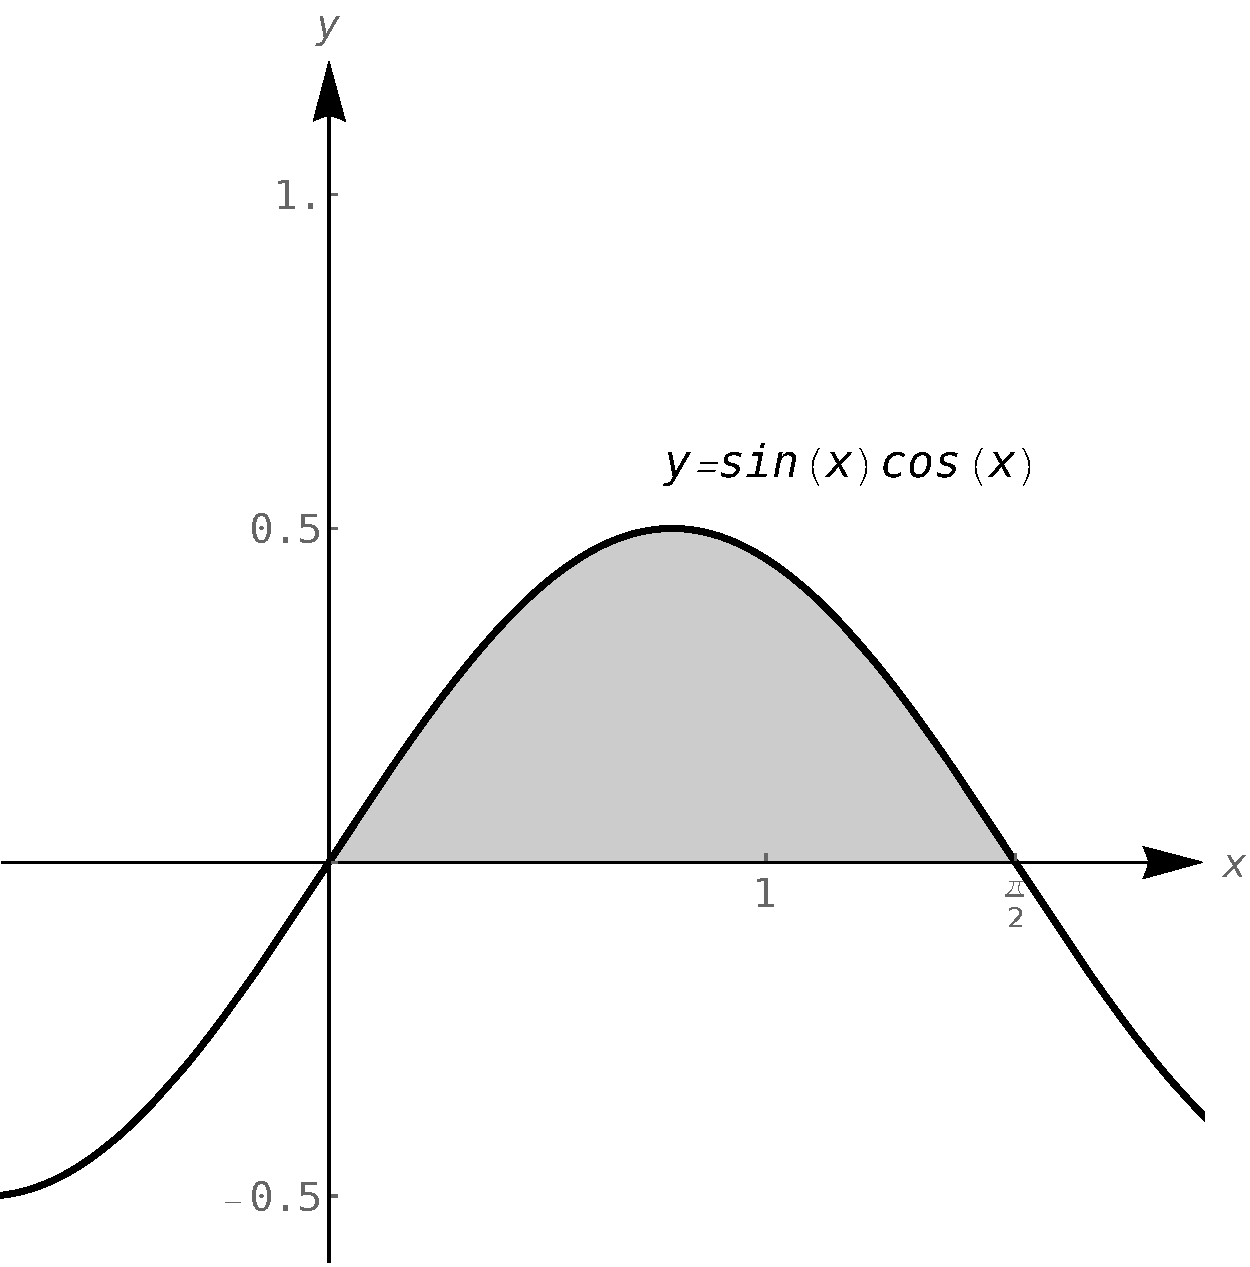
\includegraphics[width=0.4\textwidth]{fig_int_11a}}
\qquad
\subfigure[]{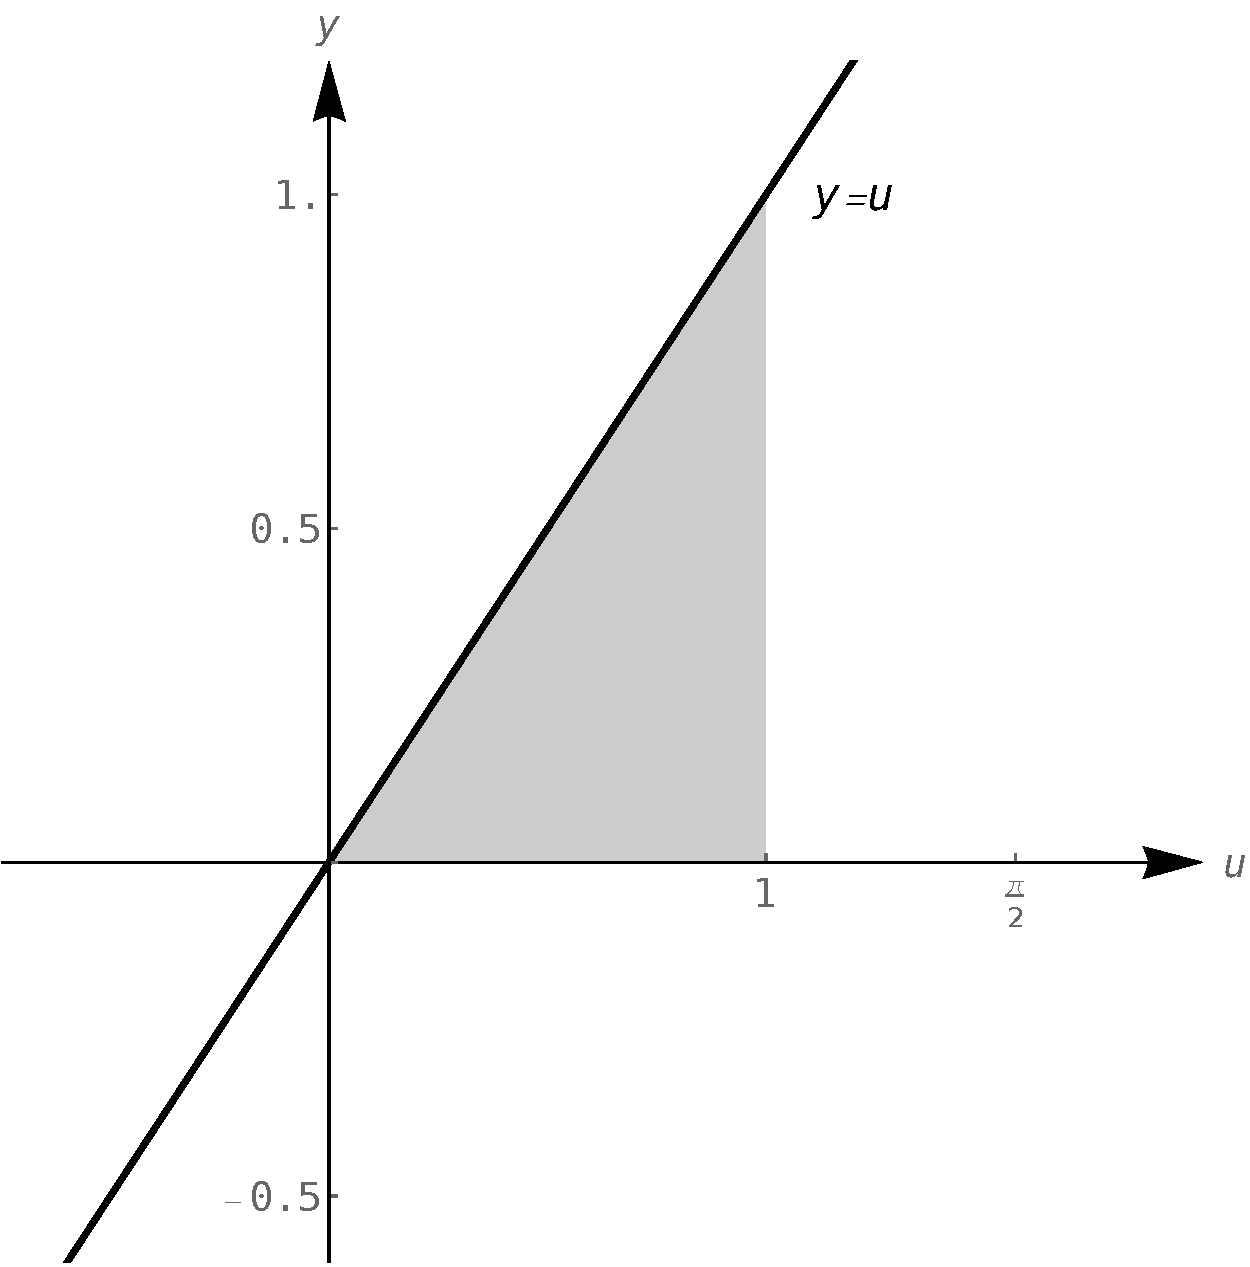
\includegraphics[width=0.4\textwidth]{fig_int_11b} }
\caption{Graphing the areas defined by the definite integrals of Example \ref{ex_subst13}.}
\label{fig_int_11}
\end{figure} 

\end{example}



\ifanalysis


\subsubsection{Tangent half-angle substitution}
The  tangent half-angle substitution, also known as the Weierstrass substitution after Karl Weierstrass, is a substitution used for finding antiderivatives of rational functions of trigonometric functions.

For this substitution we let $t = \tan\left(\frac{x}{2}\right)$. By the double-angle formula for the sine function, we get 
\allowdisplaybreaks
\begin{align*}
\sin (x)&=2\sin {\left(\dfrac {x}{2}\right)}\cos {\left(\dfrac {x}{2}\right)}\\[6pt]&=2t\cos ^{2}{\left(\dfrac {x}{2}\right)}\\[6pt]&={\dfrac {2t}{\sec ^{2}{\left(\dfrac {x}{2}\right)}}}\\[6pt]&={\dfrac {2t}{1+t^{2}}}.\end{align*} 

Similarly, by the double-angle formula for the cosine function, we easily find
\allowdisplaybreaks
\begin{align*}
\cos (x)&=1-2\sin ^{2}{\left(\dfrac {x}{2}\right)}\\[6pt]&=1-2t^{2}\cos ^{2}{\left(\dfrac {x}{2}\right)}\\[6pt]&=1-{\dfrac {2t^{2}}{\sec ^{2}{\left(\dfrac {x}{2}\right)}}}\\[6pt]&=1-{\dfrac {2t^{2}}{1+t^{2}}}\\[6pt]&={\dfrac {1-t^{2}}{1+t^{2}}}.
\end{align*}

Moreover, since 
$$
\begin{aligned}{\dfrac {dt}{dx}}&={\dfrac {1}{2}}\sec ^{2}{\left(\dfrac {x}{2}\right)}\\[6pt]&={\dfrac {1+t^{2}}{2}},
\end{aligned}
$$
we get the following expression for $dx$:
$$
\displaystyle dx={\frac {2}{1+t^{2}}}\,dt\,.
$$


\begin{example}
Evaluate the following indefinite integrals:
\begin{multicols}{2}
\begin{enumerate}
    \item $\displaystyle {\int\frac {1}{1+\sin(x)}}\,dx $
\item $\ds \int \frac{\sin(x)}{2+\cos^2(x)}\ dx$
\end{enumerate}
\end{multicols}

\pagebreak
\xhrulefill{gray}{2.5pt}Solution \xhrulefill{gray}{2.5pt}


\begin{enumerate}
\item  Using the Weierstrass substitution, we easily find
$$
\displaystyle \int{\frac {dx}{1+\sin(x)}}=\ds\int {\dfrac {1}{1+\left({\frac {2t}{1+t^{2}}}\right)}}\,\dfrac {2}{1+t^{2}}\,dt=\int{\dfrac {2}{(t+1)^{2}}}\,dt\,,
$$
where the last integral can be evaluated by a change a variables. Indeed, letting $u=t+1$, we find 
$$
\int{\dfrac {2}{(t+1)^{2}}}\,dt=\dfrac{-2}{1+t}+C\,,
$$
or in terms of the original variable $x$ where we started from:
$$
\displaystyle \int{\frac {dx}{1+\sin(x)}}=\dfrac{-2}{1+\tan\left(\frac{x}{2}\right)}+C\,.
$$
\item Again, it is clear that the Weierstrass substitution will help us out:
$$
{\displaystyle {\begin{aligned}\ds \int \frac{\sin(x)}{2+\cos^2(x)}\ dx&=\int {\frac {\left({\frac {2t}{1+t^{2}}}\right)}{2+\left({\frac {1-t^2}{1+t^{2}}}\right)^2}}\left({\frac {2}{1+t^{2}}}\,dt\right)\\
&=\int {\frac {4t}{3t^4+2t^2+3}}\,dt\,.&&\end{aligned}}}
$$
It should be clear that we can recast the last integral in order to arrive an arctangent function. This can be done, by letting $v=t^2$, to get 
$$
\ds\int {\frac {2}{3v^2+2v+3}}\,dv\,,
$$
which can be rewritten, after some algebra, as
$$
\dfrac{3}{4}\ds\int {\dfrac {1}{\left(\frac{3v+1}{2\sqrt{2}}\right)^2+1}}\,dv\,.
$$
Using the substitution $w=\frac{3v+1}{2\sqrt{2}}$, the latter integral on its turn becomes
$$
\dfrac{\sqrt{2}}{2}\ds\int\dfrac{1}{w^2+1}\,dw\,,
$$
which in terms of $v$ evaluates to
$$
\dfrac{\sqrt{2}}{2}\arctan\left(\dfrac{3v+1}{2\sqrt{2}}\right)\,.
$$
Consequently, in terms of the original variable $x$, we arrive at 
$$
\ds \int \frac{\sin(x)}{2+\cos^2(x)}\ dx=\dfrac{\sqrt{2}}{2}\arctan\left(\dfrac{3\left(\tan(\frac{x}{2})\right)^2+1}{2\sqrt{2}}\right)\,.
$$

\end{enumerate}
\end{example}


\fi



\subsection{Integration by parts}\label{sec:IBP}
\ifcourse
	\checkoddpage
\marginpar{\ifoddpage\hspace*{-1.5cm}\else\hspace*{0.25cm}\fi
\includegraphics[width=0.075\textwidth]{youtube}\\
\ifoddpage\hspace*{-1.75cm}\else\hspace*{0.1cm}\fi
\qrcode[height=1.75cm]{https://youtu.be/dh__n9FVKA0}
%\includegraphics[width=0.1\textwidth]{integration_parts}
}
\fi

Here is a simple integral that we can not yet evaluate:
$$\int x\cos(x) \,dx.$$
It's a simple matter to take the derivative of the integrand using the product rule, but there is no such rule for integrals.  However, this section introduces \textbf{integration by parts} (\textit{parti\"ele integratie}), a method of integration that is based on the product rule for derivatives. It will enable us to evaluate this integral.

The product rule says that if $u$ and $v$ are functions of $x$, then  $(uv)' = u'v + uv'$.  For simplicity, we have written $u$ for $u(x)$ and $v$ for $v(x)$.  Suppose we integrate both sides with respect to $x$.  This gives
$$\int (uv)'\,dx = \int (u'v+uv')\,dx.$$
By the fundamental theorem of calculus, the left side integrates to $uv$.  The right side can be broken up into two integrals, and we have
$$uv = \int u'v\,dx + \int uv'\,dx.$$
Solving for the second integral we have 
$$\int uv'\,dx = uv - \int u'v\,dx.$$
Using differential notation, we can write $du = u'(x)dx$ and $dv=v'(x)dx$ and the expression above can be written as follows:
\begin{equation}
\int u\,dv = uv - \int v\,du.
\label{thm:IBP}
\end{equation}
If our problem concerns a definite integral, we likewise arrive at 
$$\ds\int\limits_{x=a}^{x=b} u\ dv = uv\Big|_a^b - \ds\int\limits_{x=a}^{x=b}v\ du.$$

Typically, we try to identify $u$ and $dv$ in the integral we are given, and the key is that we usually want to choose $u$ and $dv$ so that $du$ is simpler than $u$ and $v$ is hopefully not too much more complicated than $dv$.  This will mean that the integral on the right side of the integration by parts formula, $\int v\,du$ will be simpler to integrate than the original integral $\int u\,dv$.

\begin{example}
Evaluate the following indefinite integrals:
\begin{multicols}{2}
\begin{enumerate}
\item $\displaystyle \int x^2\cos(x) \,dx$
\item  $\displaystyle \int e^x\cos(x) \,dx$
\item $\displaystyle \int \arctan(x)  \,dx$
\item $\ds \int \cos(\ln(x))\ dx$
\end{enumerate}
\end{multicols}

\pagebreak
\xhrulefill{gray}{2.5pt}Solution \xhrulefill{gray}{2.5pt}

\begin{enumerate}
\item  Let $u=x^2$ so that $dv=\cos(x)\,dx$.  Then, it follows that $du=2x\,dx$ and $v=\sin(x)$. Equation~\eqref{thm:IBP} leads to 
$$\int x^2\cos(x)\,dx = x^2\sin(x) - \int 2x\sin(x)\,dx.$$
At this point, the integral on the right is indeed simpler than the one we started with, but to evaluate it, we need to do integration by parts again. Here we choose $u=2x$ and $dv=\sin x$, so that $du=2dx$ and $v=-\cos(x)$. Through Equation~\eqref{thm:IBP} this yields:

%%%%%%.  Then $du=2\,dx$ and $v=-\cos x$.  We then get
$$\int x^2\cos(x)\,dx = x^2\sin(x) - \left(-2x\cos(x) - \int -2\cos(x)\,dx\right).$$
The integral all the way on the right is now something we can evaluate.  It evaluates to $-2\sin{x}$.  Then going through and simplifying, being careful to keep all the signs straight, our answer is
$$\int x^2\cos(x)\ dx = x^2\sin(x)  + 2x\cos(x) - 2\sin(x) + C.$$
\item This is a classic problem.  In this particular example, one can let $u$ be either $\cos(x)$ or $e^x$; we choose $u=e^x$ and hence $dv = \cos(x)\,dx$.  Then $du=e^x\,dx$ and $v=\sin(x)$ as shown below. Using Equation~\eqref{thm:IBP} yields
$$\int e^x\cos(x)\ dx = e^x\sin(x) - \int e^x\sin(x)\,dx.$$
The integral on the right is not much different than the one we started with, so it seems like we have gotten nowhere. Let us nonetheless  keep working and apply integration by parts to the new integral, using $u=e^x$ and $dv = \sin(x)\,dx$. Then we get $du=e^x\,dx$ and $v=-\cos(x)$ and this leads us to the following:
\begin{align*}
\int e^x\cos(x)\,dx &= e^x\sin(x) - \left(-e^x\cos(x) - \int -e^x\cos(x)\,dx\right)\\[0.2cm]
					&= e^x\sin(x)+ e^x\cos(x) - \int e^x\cos(x)\ dx.
\end{align*}
It seems we are back right where we started, as the right hand side contains $\int e^x\cos(x)\,dx$.  But this is actually a good thing.  

Add $\int e^x\cos(x)\ dx$ to both sides. This gives 
\begin{align*}
2\int e^x\cos(x)\ dx & = e^x\sin(x) + e^x\cos(x) \\
\intertext{Now divide both sides by 2:}
\int e^x\cos(x)\ dx & = \frac{1}{2}\big(e^x\sin(x) + e^x\cos(x)\big).
\end{align*}

Simplifying a little and adding the constant of integration, our answer is thus
$$\int e^x\cos(x)\ dx = \frac12e^x\left(\sin(x) + \cos(x)\right)+C.$$
\item  Let $u=\arctan(x)$ and $dv=dx$.  Then $du=1/(1+x^2)\,dx$ and $v=x$.  Using Equation~\eqref{thm:IBP} yields
$$\int \arctan(x) \,dx = x\arctan(x) - \int \frac x{1+x^2}\,dx.$$
The integral on the right can be solved by substitution.  Taking $u=1+x^2$, we get $du=2x\,dx$.  The integral then becomes
$$\int \arctan(x) \,dx = x\arctan(x) - \frac12\int \frac 1{u}\,du.$$
The integral on the right evaluates to $\ln|u|+C$, which becomes $\ln(1+x^2)+C$, as we may drop the absolute values as $1+x^2$ is always positive.  Therefore, the answer is
$$\int \arctan(x)\ dx = x\arctan(x) - \frac12\ln(1+x^2) + C.$$
\item The integrand contains a composition of functions, leading us to think integration by parts would be beneficial. Letting $u=\cos\left(\ln(x)\right)$, we have $du = -\sin\left(\ln(x)\right)/x\ dx$, and consequently $dv=dx$ and $v=x$. We then have
\begin{align*}
\int \cos(\ln(x))\ dx &= x\cos(\ln(x))+\int \sin(\ln(x))\ dx \\[0.2cm]
				&= x\cos(\ln(x))+x\sin(\ln(x))-\int \cos(\ln(x))\ dx\,.
				\end{align*}
So, we see that 
$$
\int \cos(\ln(x))\ dx=\frac{1}{2}x \big(\sin(\ln(x)) + \cos (\ln(x))\big)+C.
$$
\end{enumerate}
\end{example}

In general, integration by parts is useful for integrating certain products of functions, like $\int x e^x\,dx$ or $\int x^3\sin(x)\,dx$.   It is also useful for integrals involving logarithms and inverse trigonometric functions.  

As stated before, integration is generally more difficult than differentiation. We are developing tools for handling a large array of integrals, and experience will tell us when one tool is preferable/necessary over another. For instance, consider the three similar--looking integrals 
$$\int xe^x\,dx, \qquad  \int x e^{x^2}\,dx \qquad \text{and} \qquad \int xe^{x^3}\,dx.$$

While the first is calculated easily with integration by parts, the second is best approached with substitution.  Taking things one step further, the third integral has no answer in terms of elementary functions, so none of the methods we learn in calculus will get us the exact answer.

\subsection{Trigonometric integrals}\label{sec:trigint}
%\thispagestyle{empty}
Functions involving trigonometric functions are useful as they are good at describing periodic behavior. % Learning techniques to integrate such functions helps solve problems involving periodic behavior and also helps build general problem solving skills.
Here, we describe several techniques for finding antiderivatives of certain combinations of trigonometric functions.

\subsubsection{Integrals of the form $\ds \int \sin^m (x)\cos^n (x)\ dx$}
We consider integrals of the form 
$$\int \sin^m(x)\cos^n(x)\ dx,$$ 
where $m,n$ are nonnegative integers. Our strategy for evaluating these integrals is to use the identity $\cos^2(x)+\sin^2(x)=1$ to convert high powers of one trigonometric function into the other, leaving a single sine or cosine term in the integrand. This is summarized below. 
\begin{enumerate}
	\item		If $m$ is odd, then $m=2k+1$ for some integer $k$. Rewrite 
			$$ \sin^m(x) = \sin^{2k+1}(x) = \sin^{2k}(x)\sin(x) = (\sin^2(x))^k\sin(x) = (1-\cos^2(x))^k\sin(x).$$
			Then 
			$$\int \sin^m(x)\cos^n(x)\ dx = \int (1-\cos^2(x))^k\sin(x)\cos^n(x)\ dx = -\int (1-u^2)^ku^n\ du,$$
			where $u = \cos(x)$ and $du = -\sin(x)\ dx$. 
	\item		If $n$ is odd, then using substitutions similar to that outlined above we have
			$$ \int \sin^m(x)\cos^n(x)\ dx = \int u^m(1-u^2)^k\ du,$$ 
			where $u = \sin(x)$ and $du = \cos(x)\ dx$.
	\item		If both $m$ and $n$ are even, use Theorem~\ref{powerreduction} 	to reduce the degree of the integrand. Expand the result and apply (1)-(3) again.
	\end{enumerate}

Let us check out how this all works in the following examples.

\begin{example}\label{ex_trigint2}
Evaluate $$\ds \int\sin^5(x)\cos^9(x)\ dx.$$

\xhrulefill{gray}{2.5pt}Solution \xhrulefill{gray}{2.5pt}

The powers of both the sine and cosine terms are odd, therefore we can apply the techniques above to either power. We choose to work with the power of the cosine term.

We rewrite $\cos^9(x)$ as
\begin{align*} \cos^9(x) &= \cos^8(x)\cos(x) \\
				&= (\cos^2(x))^4\cos(x) \\
				&= (1-\sin^2(x))^4\cos(x) \\
				&= (1-4\sin^2(x)+6\sin^4(x)-4\sin^6(x)+\sin^8(x))\cos x.
\end{align*}

We rewrite the integral as 
$$\int\sin^5(x)\cos^9(x)\ dx = \int\sin^5(x)\big(1-4\sin^2(x)+6\sin^4(x)-4\sin^6(x)+\sin^8(x)\big)\cos(x)\ dx.$$

Now substitute using $u = \sin(x) $ and $du = \cos(x)\ dx$ to arrive at the following integral
$$  \int u^5(1-4u^2+6u^4-4u^6+u^8)\ du\,,$$
which can then be integrated:
\begin{align*} 
 \int u^5(1-4u^2+6u^4-4u^6+u^8)\ du &= \int\big(u^5-4u^7+6u^9-4u^{11}+u^{13}\big)\ du \\
				&= \frac16u^6-\frac12u^8+\frac35u^{10}-\frac13u^{12}+\frac{1}{14}u^{14}+C\\
				&= \frac16\sin^6(x)-\frac12\sin^8(x)+\frac35\sin^{10}(x)+\ldots\\
				&\phantom{=} \qquad -\frac13\sin^{12}(x)+\frac{1}{14}\sin^{14}(x)+C.
\end{align*}
\vspace{-0.5cm}
\end{example}

The work we are doing here can be a bit tedious, but the skills developed (problem solving, algebraic manipulation, etc.) are important. Nowadays problems of this sort are often solved using a computer algebra system. 
\ifmathematica
Mathematica, for instance, integrates $\int \sin^5(x)\cos^9(x)\ dx$ as 
\begin{multline*}
g(x)=-\frac{45 \cos (2 x)}{16384}-\frac{5 \cos (4 x)}{8192}+\frac{19 \cos (6
   x)}{49152}+\frac{\cos (8 x)}{4096}-\frac{\cos (10 x)}{81920}-\frac{\cos (12
   x)}{24576}-\frac{\cos (14 x)}{114688},
	\end{multline*}
\fi
\ifpython
Python, bijvoorbeeld, integreert $\int \sin^5(x)\cos^9(x)\ dx$ als 
\begin{multline*}
g(x)=-\frac{\cos^14(x)}{14} + \frac{\cos^12(x)}{6} - \frac{cos^10(x)}{10}
	\end{multline*}
\fi
which clearly has a different form than our answer in Example \ref{ex_trigint2}, which we now refer to as $f(x)$. Figure \ref{fig_int_12} shows a graph of $f$ and $g$; they are clearly not equal, but they differ only by a constant. That is $g(x) = f(x) + C$ for some constant $C$. So we have two different antiderivatives of the same function, meaning both answers are correct. 


\begin{figure}[h]
	\begin{center}
			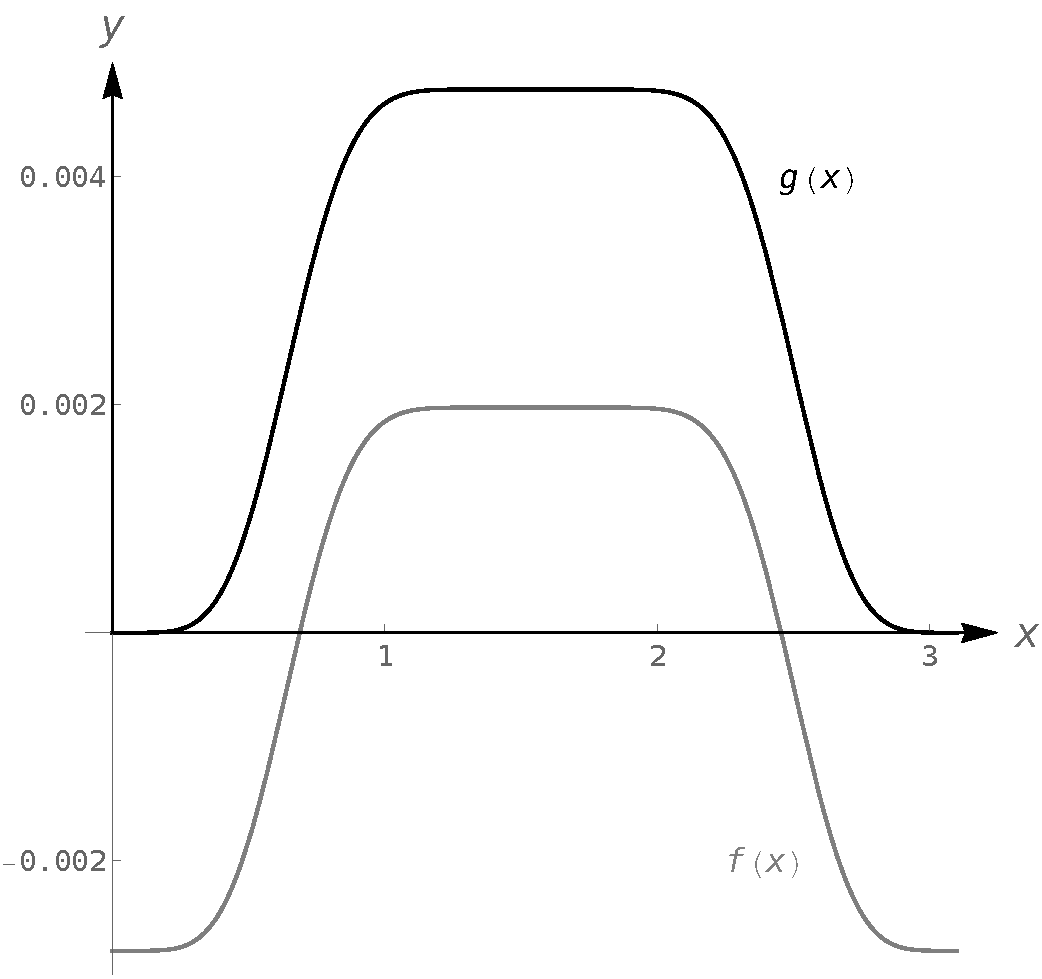
\includegraphics[width=0.5\textwidth]{fig_int_12}
	\caption{A plot of $f(x)$ and $g(x)$ from Example \ref{ex_trigint2}.}
	\label{fig_int_12}
	\end{center}
\end{figure}

\pagebreak
\begin{example}\label{ex_trigint3}
Evaluate $$\ds\int\cos^4(x)\sin^2(x)\ dx.$$

\xhrulefill{gray}{2.5pt}Solution \xhrulefill{gray}{2.5pt}

The powers of sine and cosine are both even, so we employ the power--reducing formulas and algebra as follows.
\begin{align*}
\int \cos^4(x)\sin^2(x)\ dx &= \int\left(\frac{1+\cos(2x)}{2}\right)^2\left(\frac{1-\cos(2x)}2\right)\ dx \\[0.2cm]
				&= \int\frac{1+2\cos(2x)+\cos^2(2x)}4\cdot\frac{1-\cos(2x)}2\ dx\\[0.2cm]
				&=	\int \frac18\big(1+\cos(2x)-\cos^2(2x)-\cos^3(2x)\big)\ dx
\end{align*}
The $\cos(2x)$ term is easy to integrate. The $\cos^2(2x)$ term is another trigonometric integral with an even power, requiring the power--reducing formula again. The $\cos^3(2x)$ term is a cosine function with an odd power, requiring a substitution as done before. We integrate each in turn below.

$$\int\cos(2x)\ dx = \frac12\sin(2x)+C.$$

$$\int\cos^2(2x)\ dx = \int \frac{1+\cos(4x)}2\ dx = \frac12\Big( x+\frac14\sin(4x)\Big)+C.$$

Finally, we rewrite $\cos^3(2x)$ as $$\cos^3(2x) = \cos^2(2x)\cos(2x) = \big(1-\sin^2(2x)\big)\cos(2x).$$
Letting $u=\sin(2x)$, we have $du = 2\cos(2x)\ dx$, hence
\begin{align*}
\int \cos^3(2x)\ dx &= \int\big(1-\sin^2(2x)\big)\cos(2x)\ dx\\[0.2cm]
							&= \int \frac12(1-u^2)\ du\\[0.2cm]
							&= \frac12\Big(u-\frac13u^3\Big)+C\\[0.2cm]
							&=	\frac12\Big(\sin(2x)-\frac13\sin^3(2x)\Big)+C\,.
\end{align*}

Putting all the pieces together, we have
\begin{align*}
\int \cos^4(x)\sin^2(x)\ dx &=\int \frac18\big(1+\cos(2x)-\cos^2(2x)-\cos^3(2x)\big)\ dx \\[0.2cm]
					&= \frac18\Big[x+\frac12\sin(2x)-\frac12\Big(x+\frac14\sin(4x)\Big)-\frac12\Big(\sin(2x)-\frac13\sin^3(2x)\Big)\Big]+C \\[0.2cm]
					&=\frac18\Big[\frac12x-\frac18\sin(4x)+\frac16\sin^3(2x)\Big]+C.
\end{align*}
\end{example}

\subsubsection{Integrals of products of sines and cosines of differing period}
Integrals of the form 
$$\int\sin(mx)\sin(nx)\ dx,\quad \int \cos(mx)\cos(nx)\ dx \quad \text{and}\quad\int \sin(mx)\cos(nx)\ dx$$
are best approached by first applying the product to sum formulas (Theorem~\ref{producttosum}).

\begin{example}\label{ex_trigint4}
Evaluate $$\ds\int\sin(5x)\cos(2x)\ dx.$$

\pagebreak
\xhrulefill{gray}{2.5pt}Solution \xhrulefill{gray}{2.5pt}

The application of the appropriate Simpson formula and subsequent integration are straightforward:
\begin{align*}
\int\sin(5x)\cos(2x)\ dx &= \int \frac12\Big[\sin(3x)+\sin(7x)\Big]\ dx \\[0.2cm]
												&= -\frac16\cos(3x) - \frac1{14}\cos(7x) + C
\end{align*}
\end{example}

\subsubsection{Integrals of the form $\int\tan^m(x)\sec^n(x)\ dx$.}
When evaluating integrals of the form $\int \sin^m(x)\cos^n(x)\ dx$, the Pythagorean theorem allowed us to convert even powers of sine into even powers of cosine, and vise--versa. The same basic strategy applies to integrals of the form $\int \tan^m(x)\sec^n(x)\ dx$, albeit a bit more nuanced.

Basically, if the integrand can be manipulated to separate a $\sec^2(x)$ term with the remaining secant power even, or if a $\sec (x)\tan (x)$ term can be separated with the remaining $\tan (x)$ power even, the Pythagorean theorem can be employed, leading to a simple substitution. This strategy is outlined below.


\begin{enumerate}
\item		If $n$ is even, then $n=2k$ for some integer $k$. Rewrite $\sec^nx$ as 
$$\sec^n(x) = \sec^{2k}(x) = \sec^{2k-2}(x)\sec^2(x) = (1+\tan^2(x))^{k-1}\sec^2(x).$$
Then
$$\int\tan^m(x)\sec^n(x)\ dx=\int\tan^m(x)(1+\tan^2(x))^{k-1}\sec^2(x)\ dx = \int u^m(1+u^2)^{k-1}\ du,$$
where $u = \tan (x)$ and $du = \sec^2(x)\ dx$.

\item		If $m$ is odd, then $m=2k+1$ for some integer $k$. Rewrite $\tan^m(x)\sec^n(x)$ as
\begin{eqnarray*}
\tan^m(x)\sec^n(x) &=& \tan^{2k+1}(x)\sec^n(x) = \tan^{2k}(x)\sec^{n-1}(x)\sec (x)\tan (x)\\[0.2cm]
&=& (\sec^2(x)-1)^k\sec^{n-1}(x)\sec (x)\tan (x).
\end{eqnarray*}
Then
$$\int\tan^m(x)\sec^n(x)\ dx=\int(\sec^2(x)-1)^k\sec^{n-1}(x)\sec (x)\tan (x)\ dx = \int(u^2-1)^ku^{n-1}\ du,$$
where $u = \sec (x)$ and $du = \sec (x)\tan (x)\ dx$.

\item If $n$ is odd and $m$ is even, then $m=2k$ for some integer $k$. Convert $\tan^m(x) $ to $(\sec^2(x)-1)^k$. Expand the new integrand and use Integration By Parts, with $dv = \sec^2(x)\ dx$.

\item		If $m$ is even and $n=0$, rewrite $\tan^m(x)$ as
$$\tan^m(x) = \tan^{m-2}(x)\tan^2(x) = \tan^{m-2}(x)(\sec^2(x)-1) = \tan^{m-2}(x)\sec^2(x)-\tan^{m-2}(x).$$
So
$$\int\tan^m(x)\ dx = \underbrace{\int\tan^{m-2}(x)\sec^2(x)\ dx}_{\text{\small apply rule \#1}}\quad - \underbrace{\int\tan^{m-2}(x)\ dx}_{\text{\small apply rule \#4 again}}.$$

\end{enumerate}

\begin{example}
Evaluate the following indefinite integrals:
\begin{multicols}{2}
\begin{enumerate}
\item  $\ds\int \tan^2(x)\sec^6(x)\ dx$,
\item   $\ds\int\tan^6(x)\ dx$.
\end{enumerate}
\end{multicols}

\xhrulefill{gray}{2.5pt}Solution \xhrulefill{gray}{2.5pt}

\begin{enumerate}
\item Since the power of secant is even, we use rule \#1 above  and pull out a $\sec^2(x)$ in the integrand. We convert the remaining powers of secant into powers of tangent.
\begin{align*}
\int \tan^2(x)\sec^6(x)\ dx &= \int\tan^2(x)\sec^4(x)\sec^2(x)\ dx \\[0.2cm]
		&= \int \tan^2(x)\big(1+\tan^2(x)\big)^2\sec^2(x)\ dx \\
\intertext{Now substitute, with $u=\tan(x)$, with $du = \sec^2(x)\ dx$:}
		&=\int u^2\big(1+u^2\big)^2\ du.\\
\intertext{We leave the integration and subsequent substitution to the reader. The final answer is}
		&=\frac13\tan^3(x)+\frac25\tan^5(x)+\frac17\tan^7(x)+C.
\end{align*}
\item We employ rule \#4 of the workflow outlined above. 
\begin{align*}
\int \tan^6(x)\ dx &= \int \tan^4(x)\tan^2(x)\ dx \\[0.2cm]
			&= \int\tan^4(x)\big(\sec^2(x)-1\big)\ dx\\[0.2cm]
			&= \int\tan^4(x)\sec^2(x)\ dx - \int\tan^4(x)\ dx \\
\intertext{Integrate the first integral with substitution, $u=\tan (x)$; integrate the second by employing rule \#4 again.}
			&=	\frac15\tan^5(x)-\int\tan^2(x)\tan^2(x)\ dx\\[0.2cm]
			&=	\frac15\tan^5(x)-\int\tan^2(x)\big(\sec^2(x)-1\big)\ dx \\[0.2cm]
			&= \frac15\tan^5(x) -\int\tan^2(x)\sec^2(x)\ dx + \int\tan^2(x)\ dx\\[0.2cm]
\intertext{Again, use substitution for the first integral and rule \#4 for the second.}
			&= \frac15\tan^5(x)-\frac13\tan^3(x)+\int\big(\sec^2(x)-1\big)\ dx \\[0.2cm]
			&=	 \frac15\tan^5(x)-\frac13\tan^3(x)+\tan(x) - x+C
\end{align*}
\end{enumerate}
\end{example}

These latter examples were admittedly long, with repeated applications of the same rule. Try to not be overwhelmed by the length of the problem, but rather admire how robust this solution method is. A trigonometric function of a high power can be systematically reduced to trigonometric functions of lower powers until all antiderivatives can be computed. 

\subsection{Trigonometric substitution}\label{sec:trig_sub}

\ifcourse
	\checkoddpage
\marginpar{\ifoddpage\hspace*{-1.5cm}\else\hspace*{0.25cm}\fi
\includegraphics[width=0.075\textwidth]{youtube}\\
\ifoddpage\hspace*{-1.75cm}\else\hspace*{0.1cm}\fi
\qrcode[height=1.75cm]{https://youtu.be/EV5dhv0A2wU}
%\includegraphics[width=0.1\textwidth]{substitutie_gonio}
}
 \fi
We have since learned a number of integration techniques, yet we are still unable to evaluate an integral like
\begin{equation}
\ds\int\limits_{-3}^3\sqrt{9-x^2}\ dx.
\label{vb_trig_sub}
\end{equation}
 without resorting to a geometric interpretation. This section introduces \textbf{trigonometric substitution} (\textit{goniometrische substitutie}), a method of integration that fills this gap in our integration skill. This technique works on the same principle as substitution, by setting set $x=f(\theta)$, where $f$ is a trigonometric function, and then replacing $x$ with $f(\theta)$.
 \index{ trigonometric substitution} \index[aut]{geniometrische substitutie}

For what concerns the integral given by Equation~\eqref{vb_trig_sub}, we begin by noting that $9\sin^2(\theta) + 9\cos^2(\theta) = 9$, and hence $9\cos^2(\theta) = 9-9\sin^2(\theta)$. If we let $x=3\sin(\theta)$, then $9-x^2 = 9-9\sin^2(\theta) = 9\cos^2(\theta)$. 

Setting $x=3\sin(\theta)$ gives  $dx = 3\cos(\theta)\ d\theta$. We are almost ready to substitute. We also wish to change our bounds of integration. The bound $x=-3$ corresponds to $\theta = -\pi/2$. Likewise, the bound of $x=3$ is replaced by the bound $\theta = \pi/2$. Thus

\allowdisplaybreaks
\begin{align*}
\ds\int\limits_{-3}^3\sqrt{9-x^2}\ dx &= \ds\int\limits_{-\pi/2}^{\pi/2} \sqrt{9-9\sin^2(\theta)} (3\cos(\theta))\ d\theta \\[0.2cm]
		&= \ds\int\limits_{-\pi/2}^{\pi/2} 3\sqrt{9\cos^2(\theta)} \cos(\theta)\ d\theta \\[0.2cm]
		&=\ds\int\limits_{-\pi/2}^{\pi/2} 3\left|3\cos(\theta)\right| \cos(\theta)\ d\theta.
		\intertext{}
\end{align*}
On $[-\pi/2,\pi/2]$, $\cos \theta$ is always positive, so we can drop the absolute value bars, then employ a power--reducing formula:
\begin{align*}
			&= \ds\int\limits_{-\pi/2}^{\pi/2} 9\cos^2(\theta)\ d\theta\\[0.2cm]
			&= \ds\int\limits_{-\pi/2}^{\pi/2} \frac{9}{2}\big(1+\cos(2\theta)\big)\ d\theta\\[0.2cm]
			& = \frac92 \Big(\theta +\frac12\sin(2\theta)\Big)\Bigg|_{-\pi/2}^{\pi/2}= \frac92\pi.
\end{align*}
This matches our answer in Example~\ref{ex_defint8}. 

Trigonometric substitution excels when dealing with integrands that contain $\sqrt{a^2-x^2}$, $\sqrt{x^2-a^2}$ and $\sqrt{x^2+a^2}$. The following outlines the procedure for each case. Each right triangle acts as a reference to help us understand the relationships between $x$ and $\theta$.


\begin{enumerate}
	\item[(a)] \noindent%
		\begin{minipage}[t]{.6\linewidth}%
		For integrands containing $\sqrt{a^2-x^2}$:\\[5pt]
		Let $x=a\sin(\theta)$, then $dx = a\cos(\theta)\ d\theta$.\\[5pt]	
	Thus $\theta = \arcsin(x/a)$, for $-\pi/2\leq \theta\leq \pi/2$. \\[5pt]
	On this interval, $\cos(\theta)\geq 0$, so 	$\sqrt{a^2-x^2} = a\cos(\theta).$
		\end{minipage}\qquad
	\begin{minipage}[t]{.4\linewidth}\vskip 0pt
		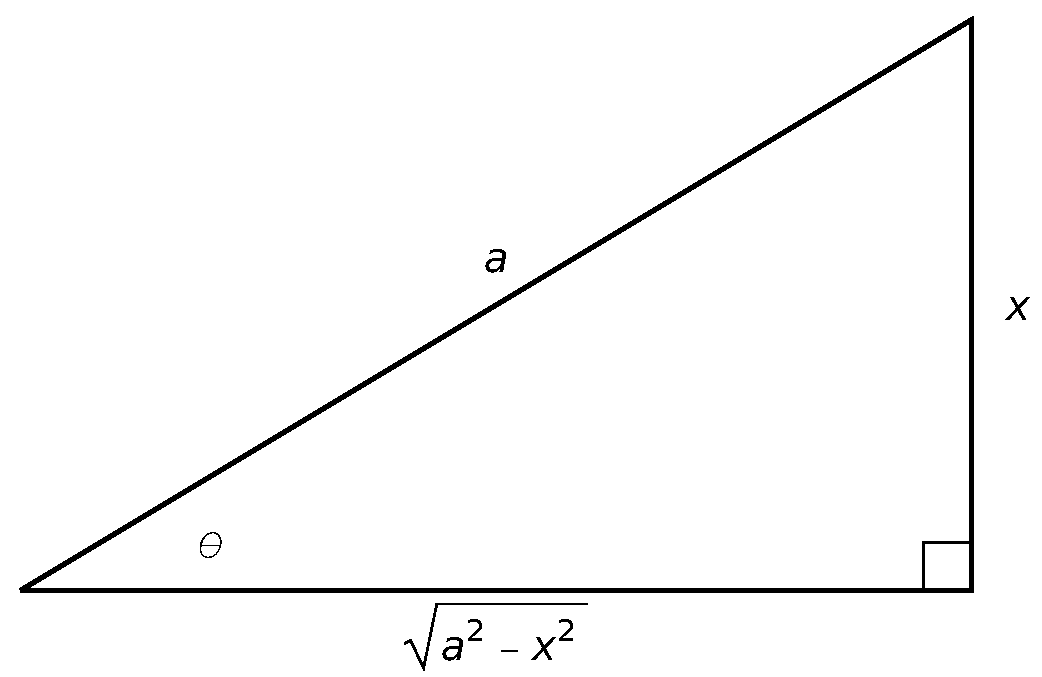
\includegraphics[width=.95\linewidth]{fig_int_13a}
		\end{minipage}
		
	\item[(b)] \noindent
	\begin{minipage}[t]{.6\linewidth}
		For integrands containing $\sqrt{x^2+a^2}$:\\[5pt]
		Let $x=a\tan(\theta)$, then $dx = a\sec^2(\theta)\ d\theta$.\\[5pt]	
	Thus $\theta = \arctan(x/a)$, for $-\pi/2 < \theta < \pi/2$. \\[5pt]	
	On this interval, $\sec(\theta)> 0$, so $\sqrt{x^2+a^2} = a\sec(\theta).$
		\end{minipage}\qquad
	\begin{minipage}[t]{.4\linewidth}\vskip 0pt
		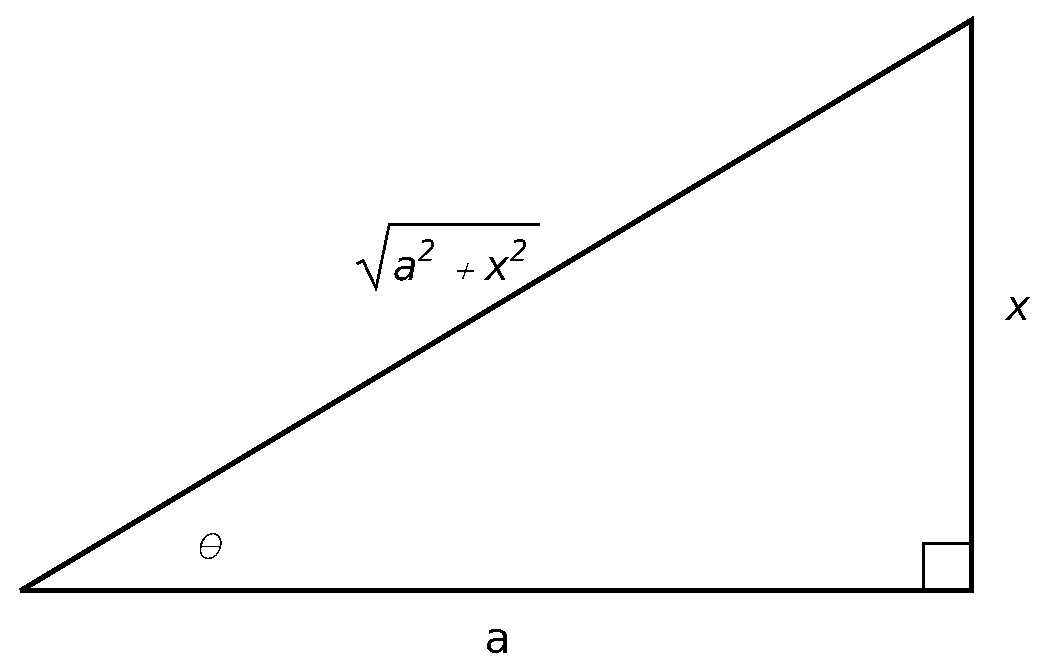
\includegraphics[width=.95\linewidth]{fig_int_13b}
		\end{minipage}
		
	\item[(c)] \noindent
	\begin{minipage}[t]{.6\linewidth}
		For integrands containing $\sqrt{x^2-a^2}$:\\[5pt]
		Let $x=a\sec(\theta)$, then $dx = a\sec(\theta)\tan(\theta)\ d\theta$.\\[5pt]	
	Thus $\theta = \arcsec(x/a)$. If $x/a\geq 1$, then $0\leq\theta<\pi/2$; if $x/a \leq -1$, then $\pi/2<\theta\leq \pi$.\\[5pt]	
	We restrict our work to where $x\geq a$, so $x/a\geq 1$, and \\ $0\leq\theta<\pi/2$. On this interval, $\tan\theta\geq 0$, so \\
	$\sqrt{x^2-a^2} = a\tan(\theta).$
		\end{minipage}\qquad
	\begin{minipage}[t]{.4\linewidth}\vskip 0pt
		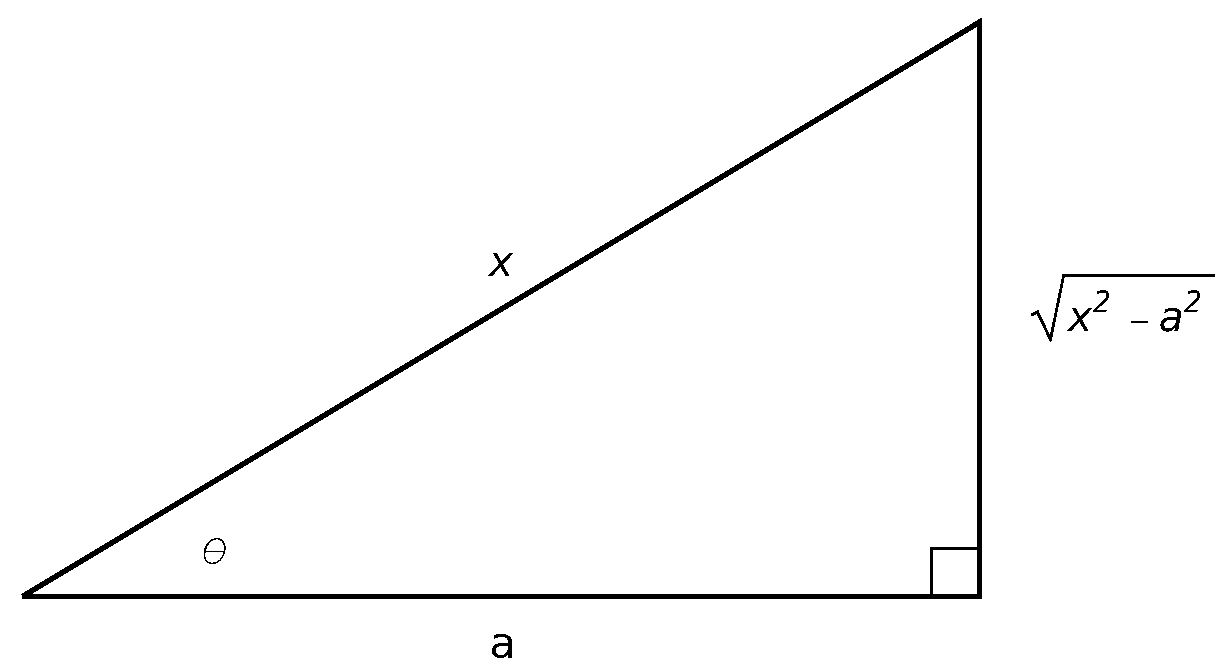
\includegraphics[width=.95\linewidth]{fig_int_13c}
		\end{minipage}	
\end{enumerate}

\begin{example}\label{ex_trigsub2}
Evaluate $$\ds \int \sqrt{4x^2-1}\ dx.$$

\xhrulefill{gray}{2.5pt}Solution \xhrulefill{gray}{2.5pt}

We start by rewriting the integrand so that it looks like $\sqrt{x^2-a^2}$ for some value of $a$:
\begin{align*}
\sqrt{4x^2-1} &= \sqrt{4\left(x^2-\frac14\right)}\\[0.2cm]
		&= 2\sqrt{x^2-\left(\frac12\right)^2}.
\end{align*}
So we have $a=1/2$, and following rule (c) from the above workflow, we set $x= \sec(\theta)/2$, and hence $dx = \sec(\theta)\tan(\theta)/2\ d\theta$. %The Key Idea also shows that $\sqrt{x^2-1/2^2} = \frac12\tan\theta$. 
We now rewrite the integral with these substitutions:
\begin{align*}
\int \sqrt{4x^2-1}\ dx &= \int 2\sqrt{x^2-\left(\frac12\right)^2}\ dx\\[0.2cm]
			&= \int 2\sqrt{\frac14\sec^2(\theta) - \frac14}\left(\frac12\sec(\theta)\tan(\theta)\right)\ d\theta\\[0.2cm]
			&=\int \sqrt{\frac14(\sec^2(\theta)-1)}\Big(\sec(\theta)\tan(\theta)\Big)\ d\theta\\[0.2cm]
			&=\int\sqrt{\frac14\tan^2(\theta)}\,\Big(\sec\theta\tan(\theta)\Big)\ d\theta\\[0.2cm]
			&=\int \frac12\tan^2(\theta)\sec(\theta)\ d\theta\\[0.2cm]
			&=\frac12\int \Big(\sec^2(\theta)-1\Big)\sec(\theta)\ d\theta\\
			&=\frac12\int \big(\sec^3(\theta) - \sec(\theta)\big)\ d\theta.
\end{align*}
We can now integrate $\sec^3(\theta)$ using integration by parts with $dv=\sec^2(\theta)$ and $u=\sec(\theta)$, finding its antiderivatives to be
$$\int \sec^3(\theta)\ d\theta = \frac12\Big(\sec(\theta)\tan(\theta) + \ln\left|\sec(\theta)+\tan(\theta)\right|\Big)+C.$$

Thus
\begin{align*}
\int \sqrt{4x^2-1}\ dx &=\frac12\int \big(\sec^3(\theta) - \sec(\theta)\big)\ d\theta\\[0.2cm]
			&= \frac12\left(\frac12\Big(\sec(\theta)\tan(\theta) + \ln\left|\sec(\theta)+\tan(\theta)\right|\Big) -\ln\left|\sec(\theta) + \tan(\theta)\right|\right) + C\\[0.2cm]
			%\end{align*}
			%\begin{align*}
			&= \frac14\left(\sec(\theta)\tan(\theta) -\ln\left|\sec(\theta)+\tan(\theta)\right|\right)+C.
\end{align*}
We are not yet done. Our original integral is given in terms of $x$, whereas our final answer, as given, is in terms of $\theta$. We need to rewrite our answer in terms of $x$. With $a=1/2$, and $x=\sec(\theta)/2$, the reference triangle in rule (c) of the above workflow shows that 
$$\tan \theta = \sqrt{x^2-\frac14}\Big/\frac12 = 2\sqrt{x^2-\frac14}\quad \text{and}\quad \sec(\theta) = 2x.$$
Thus
$$
\frac14\Big(\sec(\theta)\tan(\theta) -\ln\big|\sec(\theta)+\tan(\theta)\big|\Big)+C
$$ 
becomes
$$
				\frac14\Big(2x\, 2\sqrt{x^2-\frac14} - \ln\left|2x + 2\sqrt{x^2-\frac14}\right|\Big)+C.
$$
%or after some simplification:
%$$
%\frac14\Big(4x\sqrt{x^2-\frac14} - \ln\big|2x + 2\sqrt{x^2-\frac14}\big|\Big)+C.
%$$
The final answer hence is:
$$
\int \sqrt{4x^2-1}\ dx = \frac14\Big(4x\sqrt{x^2-\frac14} - \ln\left|2x + 2\sqrt{x^2-\frac14}\right|\Big)+C.
$$
\end{example}

It is important to realize that trigonometric substitution can be applied in many situations, even those not of the form $\sqrt{a^2-x^2}$, $\sqrt{x^2-a^2}$ or $\sqrt{x^2+a^2}$. This is illustrated in the following example. 

\begin{example}\label{ex_trigsub7}
Evaluate $$\ds\int\frac1{(x^2+6x+10)^2}\ dx.$$

\xhrulefill{gray}{2.5pt}Solution \xhrulefill{gray}{2.5pt}

We start by completing the square, then make the substitution $u=x+3$, followed by the trigonometric substitution of $u=\tan(\theta)$:
\begin{align}
\int \frac1{(x^2+6x+10)^2}\ dx =\int \frac1{\big((x+3)^2+1\big)^2}\ dx&= \int \frac1{(u^2+1)^2}\ du. \notag
\intertext{Now make the substitution $u=\tan(\theta)$, $du=\sec^2(\theta)\ d\theta$:}
 \int \frac1{(u^2+1)^2}\ du  &=	\int \frac1{(\tan^2(\theta)+1)^2}\sec^2(\theta)\ d\theta\notag\\[0.2cm]
	&= \int\frac 1{(\sec^2(\theta))^2}\sec^2(\theta)\ d\theta\notag\\[0.2cm]
	&= \int \cos^2(\theta)\ d\theta.\notag
	\intertext{Applying a power reducing formula, we have}
\int \cos^2(\theta)\ d\theta  & = \int \left(\frac12 +\frac12\cos(2\theta)\right)\ d\theta \notag\\[0.2cm]
	&= \frac12\theta + \frac14\sin(2\theta) + C.\label{eq:extrigsub7}
\end{align}
We need to return to the variable $x$. As $u=\tan(\theta)$, $\theta = \arctan(u)$. Using the identity \linebreak $\sin(2\theta) = 2\sin(\theta)\cos(\theta)$ and using the reference triangle found in rule (b) of the workflow above, we have 
$$\frac14\sin(2\theta) = \frac12\frac u{\sqrt{u^2+1}}\,\frac 1{\sqrt{u^2+1}} = \frac12\frac u{u^2+1}.$$
Finally, we return to $x$ with the substitution $u=x+3$. We start with the expression in Equation~ \eqref{eq:extrigsub7}:
\begin{align*}
\frac12\theta + \frac14\sin(2\theta) + C &= \frac12\arctan(u) + \frac12\frac{u}{u^2+1}+C\\
				&= \frac12\arctan(x+3) + \frac{x+3}{2(x^2+6x+10)}+C.
\end{align*}
Stating our final result in one line:
$$\int\frac1{(x^2+6x+10)^2}\ dx=\frac12\arctan(x+3) + \frac{x+3}{2(x^2+6x+10)}+C.$$
\end{example}


Finally, it should be mentioned that given a definite integral that can be evaluated using trigonometric substitution, we could first evaluate the corresponding indefinite integral and then evaluate using the original bounds. It is much more straightforward, though, to change the bounds as we substitute.

\subsection{Partial fraction decomposition}\label{sec:partial_fraction}


\ifcourse
	\checkoddpage
\marginpar{\ifoddpage\hspace*{-1.5cm}\else\hspace*{0.25cm}\fi
\includegraphics[width=0.075\textwidth]{youtube}\\
\ifoddpage\hspace*{-1.75cm}\else\hspace*{0.1cm}\fi
\qrcode[height=1.75cm]{https://youtu.be/Mt92Ozs7aJg}
%\includegraphics[width=0.1\textwidth]{figures/Int/partial_fractions.png}
}
 \fi
Here we investigate the antiderivatives of rational functions. Recall that rational functions are functions of the form $f(x)= \frac{p(x)}{q(x)}$, where $p(x)$ and $q(x)$ are polynomials and $q(x)\neq 0$. 

Consider the integral 
$$\ds\int \frac{1}{x^2-1}\ dx.$$
 We do not have a simple formula for this. It can be evaluated using trigonometric substitution, but note how the integral is easy to evaluate once we realize:
$$\frac{1}{x^2-1} = \frac{1/2}{x-1} - \frac{1/2}{x+1}.$$
Thus 
\begin{align*}
\int\frac{1}{x^2-1}\ dx &= \int\frac{1/2}{x-1}\ dx - \int\frac{1/2}{x+1}\ dx \\
			&= \frac12\ln|x-1| - \frac12\ln|x+1| + C.
\end{align*}
Here, we will learn how to decompose fractions like  $$\frac{1}{x^2-1}.$$

We start with a rational function 
$$f(x)=\frac{p(x)}{q(x)},$$
where $p$ and $q$ do not have any common factors and the degree of $p$ is less than the degree of $q$. It can be shown that any polynomial, and hence $q$, can be factored into a product of real linear and irreducible quadratic terms. The following workflow states how to \textbf{decompose a rational function into partial fractions} (\textit{splitsing in partieelbreuken}) as a sum of rational functions whose denominators are all of lower degree than $q$.
%\clearpage

\begin{enumerate}
	\item	\textbf{Linear Terms:} Let $(x-a)$ divide $q(x)$, where $(x-a)^n$ is the highest power of $(x-a)$ that divides $q(x)$. Then the decomposition of $f(x)$ will contain the sum
	$$\frac{A_1}{(x-a)} + \frac{A_2}{(x-a)^2} + \cdots +\frac{A_n}{(x-a)^n}.$$
	\item		\textbf{Quadratic Terms:} Let ($x^2+bx+c$) divide $q(x)$, where $(x^2+bx+c)^n$ is the highest power of ($x^2+bx+c$) that divides $q(x)$. Then the decomposition of $f(x)$ will contain the sum 
	$$\frac{B_1x+C_1}{x^2+bx+c}+\frac{B_2x+C_2}{(x^2+bx+c)^2}+\cdots+\frac{B_nx+C_n}{(x^2+bx+c)^n}.$$
	\end{enumerate}
	To find the coefficients $A_i$, $B_i$ and $C_i$:
	\begin{enumerate}
	\item	Multiply all fractions by $q(x)$, clearing the denominators. Collect like terms.
	\item		Equate the resulting coefficients of the powers of $x$ and solve the resulting system of linear equations.
	\end{enumerate}

\begin{example}\label{ex_pf2}
Perform the partial fraction decomposition of
$$\ds \frac{1}{x^2-1}.$$

\xhrulefill{gray}{2.5pt}Solution \xhrulefill{gray}{2.5pt}

The denominator factors into two linear terms: $x^2-1 = (x-1)(x+1)$. Thus 
$$\frac{1}{x^2-1} = \frac{A}{x-1} + \frac{B}{x+1}.$$
To solve for $A$ and $B$, first multiply through by $x^2-1 = (x-1)(x+1)$:
\begin{align*}
1 &= \frac{A(x-1)(x+1)}{x-1}+\frac{B(x-1)(x+1)}{x+1} \\[0.2cm]
	&= A(x+1) + B(x-1)\\[0.2cm]
	&= Ax+A + Bx-B \\[0.2cm]
	&= (A+B)x + (A-B).
\end{align*}
The next step is key. Note the equality we have:
$$1 = (A+B)x+(A-B).$$
For clarity's sake, rewrite the left hand side as
$$0x+1 = (A+B)x+(A-B).$$
On the left, the coefficient of the $x$ term is 0; on the right, it is $(A+B)$. Since both sides are equal, we must have that $0=A+B$. 

Likewise, on the left, we have a constant term of 1; on the right, the constant term is $(A-B)$. Therefore we have $1=A-B$.

We have two linear equations with two unknowns. This one is easy to solve by hand, leading to 
$$\begin{cases} A+B = 0 \\ A-B = 1 \end{cases} \quad\Rightarrow\quad \begin{cases} A=1/2 \\ B = -1/2.\end{cases}$$
Thus $$\frac{1}{x^2-1} = \frac{1/2}{x-1}-\frac{1/2}{x+1}.$$
\end{example}
\ifmathematica
Clearly, it can become rather tedious to do a a partial fraction decomposition by hand if one is confronted with a more complex rational fraction. Luckily, we can resort in such cases to Mathematica, which can accomplish this with the command \lstinline{Apart}. For instance, for what concerns the rational function in Example~\eqref{ex_pf2}, we should proceed as follows. 
	\begin{mdframed}[default,backgroundcolor=gray!40,roundcorner=8pt]
\begin{mmaCell}[morefunctionlocal={x}]{Input}
  Apart[1/(x^2 - 1), x]
\end{mmaCell}
The second argument of the command \lstinline{Apart} is nothing but the variable at stake. 
\begin{mmaCell}{Output}
  \mmaFrac{1}{2 (-1+x)}-\mmaFrac{1}{2 (1+x)}
\end{mmaCell}
\end{mdframed}
\index{\lstinline{Apart}}\index[aut]{\lstinline{Apart}}
\fi
\ifpython
Clearly, it can become rather tedious to do a a partial fraction decomposition by hand if one is confronted with a more complex rational fraction. Luckily, we can resort in such cases to Python, which can accomplish this with the command \lstinline{Apart}. For instance, for what concerns the rational function in Example~\eqref{ex_pf2}, we should proceed as follows. 
\begin{pyin}
from sympy import symbols, apart
x = symbols('x')
apart(1/(x**2 - 1), x)
\end{pyin}
Het tweede argument van het commando \lstinline{apart} is niets anders dan de veranderlijke. 
\begin{pyout}
-\frac{1}{2(x+1)} + \frac{1}{2(x-1)}
\end{pyout}
\fi
\begin{example}
Evaluate the following indefinite integrals:
\begin{multicols}{2}
\begin{enumerate}
\item  $\ds\int\frac{1}{(x-1)(x+2)^2}\ dx$,
\item  $\ds \int \frac{x^3}{(x-5)(x+3)}\ dx$\ifcalculus .\fi\ifanalysis,\fi
\ifanalysis \item $\ds \int \frac{2+\sin(x)}{3+\cos(x)}\ dx$. \fi
\end{enumerate}
\end{multicols}

\ifcalculus\pagebreak\fi
\xhrulefill{gray}{2.5pt}Solution \xhrulefill{gray}{2.5pt}

\begin{enumerate}
\item  We decompose the integrand as follows:
$$\frac{1}{(x-1)(x+2)^2} = \frac{A}{x-1} + \frac{B}{x+2} + \frac{C}{(x+2)^2}.$$
To solve for $A$, $B$ and $C$, we multiply both sides by $(x-1)(x+2)^2$ and collect like terms:
\begin{align}
1 &= A(x+2)^2 + B(x-1)(x+2) + C(x-1)\label{eq:pf3}\\
	&= Ax^2+4Ax+4A + Bx^2 + Bx-2B + Cx-C \notag \\
	&= (A+B)x^2 + (4A+B+C)x + (4A-2B-C).\notag
\end{align}

We have $$0x^2+0x+ 1 = (A+B)x^2 + (4A+B+C)x + (4A-2B-C)\,,$$
leading to the equations 
$$
\left\{\begin{array}{rcl}
A+B &=& 0\\
4A+B+C &=& 0\\
4A-2B-C &=& 1
\end{array}
\right.\qquad\Leftrightarrow\qquad
\left\{\begin{array}{rcl}
A &=& \dfrac{1}{9}\\[0.2cm]
B&=& -\dfrac{1}{9}\\[0.2cm]
C &=& -\dfrac{1}{3}
\end{array}
\right.
$$
Thus 
$$\int\frac{1}{(x-1)(x+2)^2}\ dx = \int \frac{1/9}{x-1}\ dx + \int \frac{-1/9}{x+2}\ dx + \int \frac{-1/3}{(x+2)^2}\ dx.$$

Each can be integrated with a simple substitution with $u=x-1$ or $u=x+2$. The end result is
$$\int\frac{1}{(x-1)(x+2)^2}\ dx = \frac19\ln|x-1| -\frac19\ln|x+2| +\frac1{3(x+2)}+C.$$
\item  Since the degree of the numerator is now higher than the one of the denominator, we begin by using polynomial division to reduce the degree of the numerator (see Section~\ref{sec_pol}). Doing so, we arrive at
$$\frac{x^3}{(x-5)(x+3)} = x+2+\frac{19x+30}{(x-5)(x+3)}.$$
Consequently, we can rewrite the new rational function as:
$$\frac{19x+30}{(x-5)(x+3)} = \frac{A}{x-5} + \frac{B}{x+3},$$ for appropriate values of $A$ and $B$. Clearing denominators, we have 
\begin{align*}
19x+30 &= A(x+3) + B(x-5)\\
			&= (A+B)x + (3A-5B).
\end{align*}

This implies that:
$$
\begin{cases}
19= A+B \\
30= 3A-5B.
\end{cases}
\qquad\Leftrightarrow\qquad
\begin{cases}
A=\dfrac{125}{8}\\[0.2cm]
B=\dfrac{27}{8}.
\end{cases}
$$

We can now integrate:
\begin{align*}
\int \frac{x^3}{(x-5)(x+3)}\ dx &= \int\left(x+2+\frac{125/8}{x-5}+\frac{27/8}{x+3}\right)\ dx \\[0.2cm]
					&= \frac{x^2}2 + 2x + \frac{125}{8}\ln|x-5| + \frac{27}8\ln|x+3| + C.
\end{align*}

\item We observe that we are confronted with a rational function of trigonometric functions, so we first of all resort to the Weierstrass substitution. This leads to the following integral
$$
2\ds \int \frac{t^2+t+1}{(t^2+2)(t^2+1)}\ dt\,,
$$
which can be finished off using partial fraction decomposition. In this way, we get
$$
2\ds \int \frac{t^2+t+1}{(t^2+2)(t^2+1)}\ dt=2\ds \int \frac{1-t}{t^2+2}\ dt+\int \frac{t}{t^2+1}\,dt\,.
$$
Hence, we arrive at
$$
2\ds \int \frac{t^2+t+1}{(t^2+2)(t^2+1)}\ dt=\dfrac{1}{\sqrt{2}}\arctan\left(\dfrac{t}{\sqrt{2}}\right)-\dfrac{1}{2}\ln\left(t^2+2\right)+\dfrac{1}{2}\ln\left(t^2+1\right)+C\,,
$$
where $t=\tan(x/2)$.

\end{enumerate}
\end{example}

We conclude our discussion of partial fraction decomposition with a final example that combines several of the techniques we encountered earlier in this section. 

\begin{example}\label{ex_pf5}
Evaluate $$\ds \int\frac{7x^2+31x+54}{(x+1)(x^2+6x+11)}\ dx.$$

\xhrulefill{gray}{2.5pt}Solution \xhrulefill{gray}{2.5pt}

The degree of the numerator is less than the degree of the denominator, so we have:
\begin{align*}
\frac{7x^2+31x+54}{(x+1)(x^2+6x+11)} &= \frac{A}{x+1} + \frac{Bx+C}{x^2+6x+11}. \\
\intertext{Now clear the denominators.}
7x^2+31x+54 &= A(x^2+6x+11) + (Bx+C)(x+1)\\
					&= (A+B)x^2 + (6A+B+C)x + (11A+C).
\end{align*}
This implies that:
$$
\begin{cases*}
				7=A+B\\
				31 = 6A+B+C\\
				54 = 11A+C.
\end{cases*}
\qquad\Leftrightarrow\qquad
\begin{cases*}
				A=5\\
				B= 2\\
				C = -1.
\end{cases*}
$$
Thus
$$\int\frac{7x^2+31x+54}{(x+1)(x^2+6x+11)}\ dx = \int\left(\frac{5}{x+1} + \frac{2x-1}{x^2+6x+11}\right)\ dx.$$

The first term of this new integrand is easy to evaluate; it leads to a $5\ln|x+1|$ term. The second term is not hard, but takes several steps and uses substitution techniques.

The integrand $\ds \frac{2x-1}{x^2+6x+11}$ has a quadratic in the denominator and a linear term in the numerator. This leads us to try substitution. Let $u = x^2+6x+11$, so $du = (2x+6)\ dx$. The numerator is $2x-1$, not $2x+6$, but we can get a $2x+6$ term in the numerator by adding 0 in the form of ``$7-7$.''
\begin{align*}
\frac{2x-1}{x^2+6x+11} &= \frac{2x-1+7-7}{x^2+6x+11} \\[0.2cm]
					&= \frac{2x+6}{x^2+6x+11} - \frac{7}{x^2+6x+11}.
\end{align*}
We can now integrate the first term with substitution, leading to a $\ln|x^2+6x+11|$ term. The final term can be integrated using arctangent. First, complete the square in the denominator:
$$\frac{7}{x^2+6x+11} = \frac{7}{(x+3)^2+2}.$$
An antiderivative of the latter term can be found using Equation~\eqref{arctan_direct} and substitution:
$$\int \frac{7}{x^2+6x+11}\ dx = \frac{7}{\sqrt{2}}\arctan\left(\frac{x+3}{\sqrt{2}}\right)+C.$$

Let's start at the beginning and put all of the steps together.
\begin{align*}
\int\frac{7x^2+31x+54}{(x+1)(x^2+6x+11)}\ dx &= \int\left(\frac{5}{x+1} + \frac{2x-1}{x^2+6x+11}\right)\ dx\\[0.2cm] 
			&= \int\frac{5}{x+1}\ dx  + \int\frac{2x+6}{x^2+6x+11}\ dx -\int\frac{7}{x^2+6x+11}\ dx \\[0.2cm]
			&= 5\ln|x+1|+ \ln\left|x^2+6x+11\right| -\frac{7}{\sqrt{2}}\arctan\left(\frac{x+3}{\sqrt{2}}\right)+C
\end{align*}%\normalsize
It is important to remember that one is not expected to see the final answer immediately after seeing the problem. Rather, given the initial problem, we break it down into smaller problems that are easier to solve. The final answer is a combination of the answers of the smaller problems.
\end{example}


Partial fraction decomposition is an important tool when dealing with rational functions. Note that at its heart, it is a technique of algebra, not calculus, as we are rewriting a fraction in a new form. Still, it is very useful in the realm of calculus as it lets us evaluate a certain set of complicated integrals.

\begin{remark}[Integral equations]
In Chapter~\ref{chap_diff}, we encountered differential equations, which are equations  that relate some function with its derivatives. Likewise, we can formulate integral equations, which are equations in which an unknown function appears under an integral sign. Consider, for instance, the following integral equation:
$$
f(x)=e^{-x}-\dfrac{1}{2}+\dfrac{1}{2}e^{-x-1}+\dfrac{1}{2}\ds\int\limits_0^1(x+1)e^{-xy}f(y)\,dy.
$$
Its solution is $f(x)=e^{-x}$, which can verified easily. 

Just are the differential equations, integral equations are omnipresent in physics and engineering. For instance, Maxwell's equations of electromagnetism can be formulated in integral form. 


\end{remark}


\section{Improper Integration}\label{sec:improper_integration}

Consider the following definite integrals:
\begin{multicols}{3}
\begin{itemize}
\item	$\ds \int\limits_0^{100}\frac1{1+x^2}\ dx \approx 1.5608,$
\item	$\ds \int\limits_0^{1000}\frac1{1+x^2}\ dx \approx 1.5698,$
\item	$\ds \int\limits_0^{10,000}\frac1{1+x^2}\ dx \approx 1.5707.$
\end{itemize}
\end{multicols}


Notice how the integrand is $1/(1+x^2)$ in each integral. It is sketched in Figure~\ref{fig_int_14}. As the upper bound gets larger, one would expect the area under the curve would also grow. While the definite integrals do increase in value as the upper bound grows, they are not  increasing by much. In fact, consider:
$$\ds \int\limits_0^b \frac{1}{1+x^2}\ dx = \arctan(x)\Big|_0^b = \arctan(b)-\arctan(0) = \arctan(b).$$
As $b\rightarrow +\infty$, $\arctan(b) \rightarrow \pi/2.$ Therefore it seems that as the upper bound $b$ grows, the value of the concerned definite integral  approaches $\pi/2\approx 1.5708$. This should strike the reader as being a bit amazing: even though the curve extends to infinity, it has a finite amount of area underneath it.





When we defined the definite integral $\int_a^b f(x)\ dx$ in Definition~\ref{def:def_int}, we made two stipulations:
	\begin{enumerate}
	\item		The interval over which we integrated, $[a,b]$, was a finite interval, and
	\item		The function $f(x)$ was continuous on $[a,b]$ (ensuring that the range of $f$ was finite).
	\end{enumerate}
	
In this section we consider integrals where one or both of the above conditions do not hold. Such integrals are called \textbf{improper integrals} (\textit{oneigenlijke integraal})


\begin{figure}[h]
	\begin{center}
			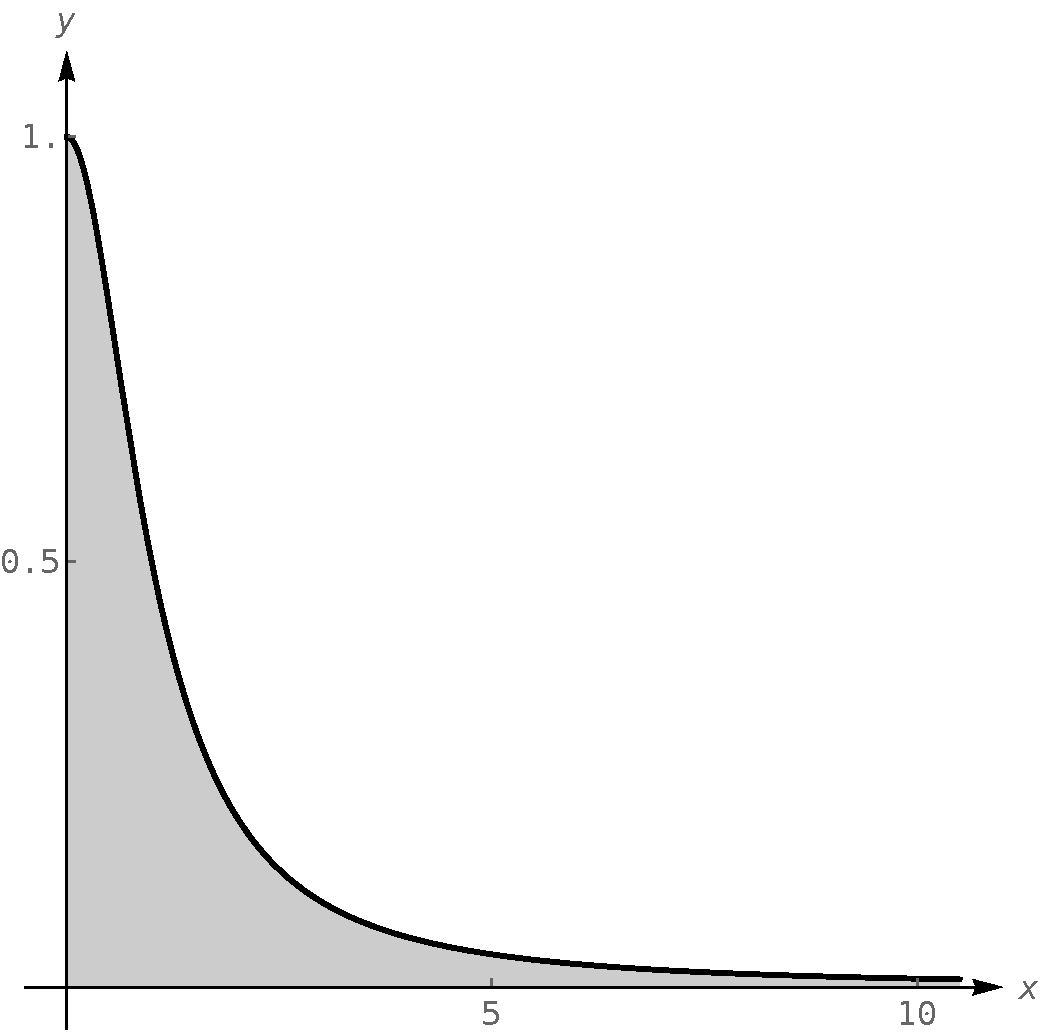
\includegraphics[width=0.4\textwidth]{fig_int_14}
	\caption{Graphing $\ds f(x)=\frac{1}{1+x^2}$.}
	\label{fig_int_14}
	\end{center}
\end{figure}

\subsection{Improper integrals with infinite bounds}
We start with a definition of Improper integrals with infinite bounds. 

\begin{definition}[Improper integrals with infinite bounds]\label{def:imp_int1}
\begin{enumerate}
\item		Let $f$ be a continuous function on $[a,+\infty\left[\right.$. Define \index{integration!improper}\index{improper integration}\index[aut]{integraal ! oneigenlijk}\index[aut]{oneigenlijke integraal} %\small
$$\ds \int\limits_a^{+\infty} f(x)\ dx \quad \text{to be}\quad \lim_{b\to+\infty}\ds \int\limits_a^b f(x)\ dx.$$

\item		Let $f$ be a continuous function on $\left.\right]-\infty,b]$. Define %\small
$$\ds \int\limits_{-\infty}^b f(x)\ dx \quad \text{to be}\quad \lim_{a\to-\infty}\ds \int\limits_a^b f(x)\ dx.$$

\item		Let $f$ be a continuous function on $\mathbb{R}$. Let $c$ be any real number; define %\small
$$\ds \int\limits_{-\infty}^{+\infty} f(x)\ dx \quad \text{to be}\quad \lim_{a\to-\infty}\ds \int\limits_a^c f(x)\ dx\ +\ \lim_{b\to+\infty}\ds \int\limits_c^b f(x)\ dx.$$
\end{enumerate}
An improper integral is said to converge if its corresponding limit exists (is finite); otherwise, it diverges. The improper integral in part 3 converges if and only if both of its limits exist.
\end{definition}

\begin{example}\label{ex_impint1}
Evaluate the following improper integrals:

%\begin{minipage}[t]{.5\textwidth}
\begin{multicols}{3}
\begin{enumerate}
\item		$\ds \int\limits_1^{+\infty} \frac1{x^2}\ dx$,
\item		$\ds \int\limits_1^{+\infty} \frac1x\ dx$,
\item		$\ds \int\limits_{-\infty}^{+\infty} \frac1{1+x^2}\ dx$.
\end{enumerate}
\end{multicols}
%\end{minipage}
%\begin{minipage}[t]{.5\textwidth}
%\begin{enumerate}\addtocounter{enumi}{2}
%\item		$\ds\int_{-\infty}^\infty \frac1{1+x^2}\ dx$
%\end{enumerate}
%\end{minipage}


\xhrulefill{gray}{2.5pt}Solution \xhrulefill{gray}{2.5pt}


\begin{enumerate}
\item		\hfill\allowdisplaybreaks\begin{align}[t] \ds \int\limits_1^{+\infty} \frac{1}{x^2}\ dx\  =\ \lim_{b\to+\infty} \ds \int\limits_1^b\frac1{x^2}\ dx\  &=\ \lim_{b\to+\infty} \frac{-1}{x}\Big|_1^b \\[0.2cm]
 %&= \lim_{b\to+\infty} \frac{-1}{x}\Big|_1^b \\
 &= \lim_{b\to+\infty} \frac{-1}{b} + 1=1.\end{align}\hfill\null

A graph of the area defined by this integral is given in Figure \ref{fig_int_15a}. 
\ifmathematica
In Mathematica, this result can be checked as follows: 
	\begin{mdframed}[default,backgroundcolor=gray!40,roundcorner=8pt]
\begin{mmaCell}[morefunctionlocal={x}]{Input}
  Integrate[1/x^2, {x, 1, +Infinity}]
\end{mmaCell}
\begin{mmaCell}{Output}
  1
\end{mmaCell}
\end{mdframed}
 \index{\lstinline{Integrate}}\index[aut]{\lstinline{Integrate}}
 \fi
 
\ifpython
In Python, this result can be checked as follows: 
\begin{pyin}
from sympy import symbols, integrate, oo
x = symbols('x')
integrate(1/x**2, (x, 1, oo))
\end{pyin}
\begin{pyout}
1
\end{pyout}
\fi
 
\item		\hfill$\begin{aligned}[t]%
			\ds \int\limits_1^\infty \frac1x\ dx & = \lim_{b\to+\infty}\ds \int\limits_1^b\frac1x\ dx \\[0.2cm]
						&= \lim_{b\to+\infty} \ln |x|\Big|_1^b \\[0.2cm]
						&= \lim_{b\to+\infty} \ln (b)\\
						&= +\infty.
	\end{aligned}$\hfill\null
	
The limit does not exist, hence the concerned improper integral  diverges. Compare the graphs in Figures \ref{fig_int_15a} and \ref{fig_int_15b}; notice how the graph of $f(x) = 1/x$ is noticeably larger. This difference is enough to cause the improper integral to diverge.

\begin{figure}[H]
\centering
%\raisebox{0.5cm}{
\subfigure[\label{fig_int_15a}]{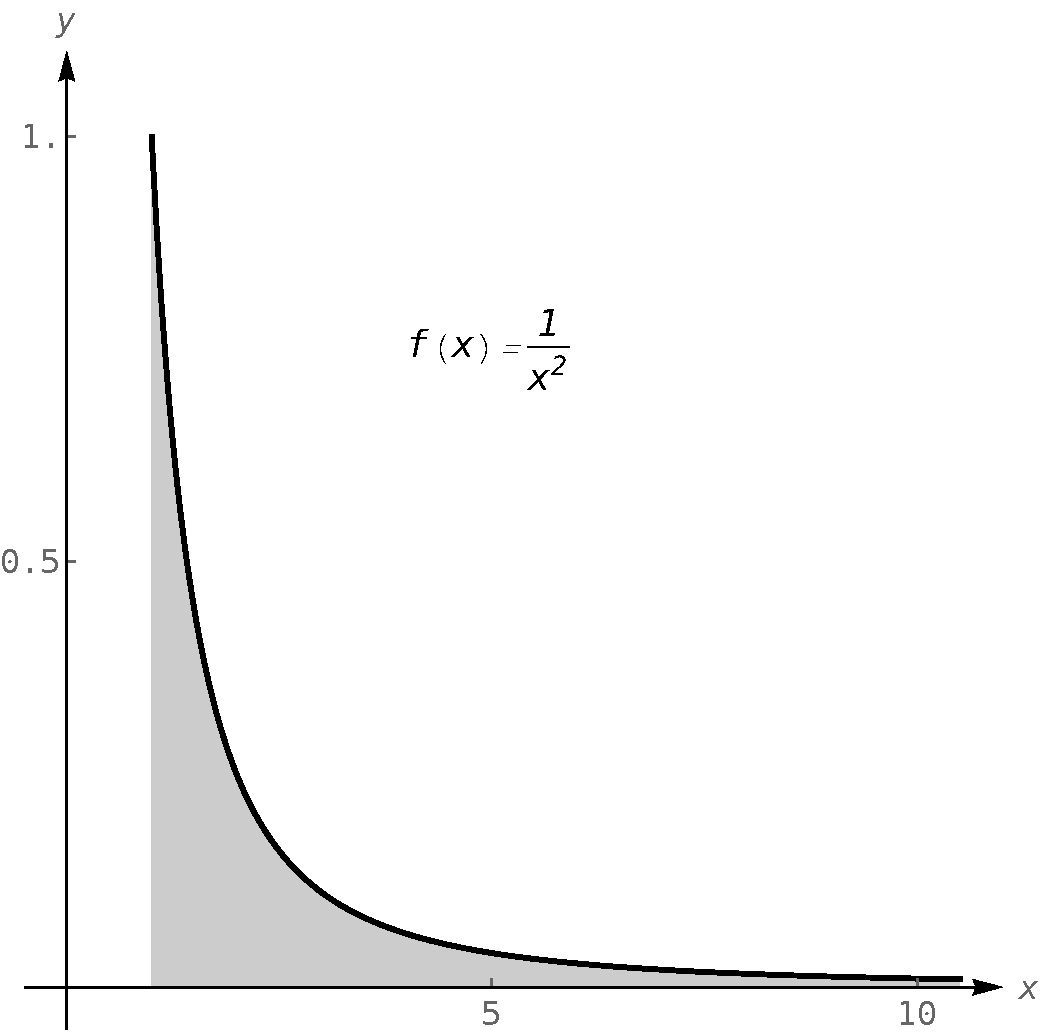
\includegraphics[width=0.3\textwidth]{fig_int_15a}}
\qquad
\subfigure[\label{fig_int_15b}]{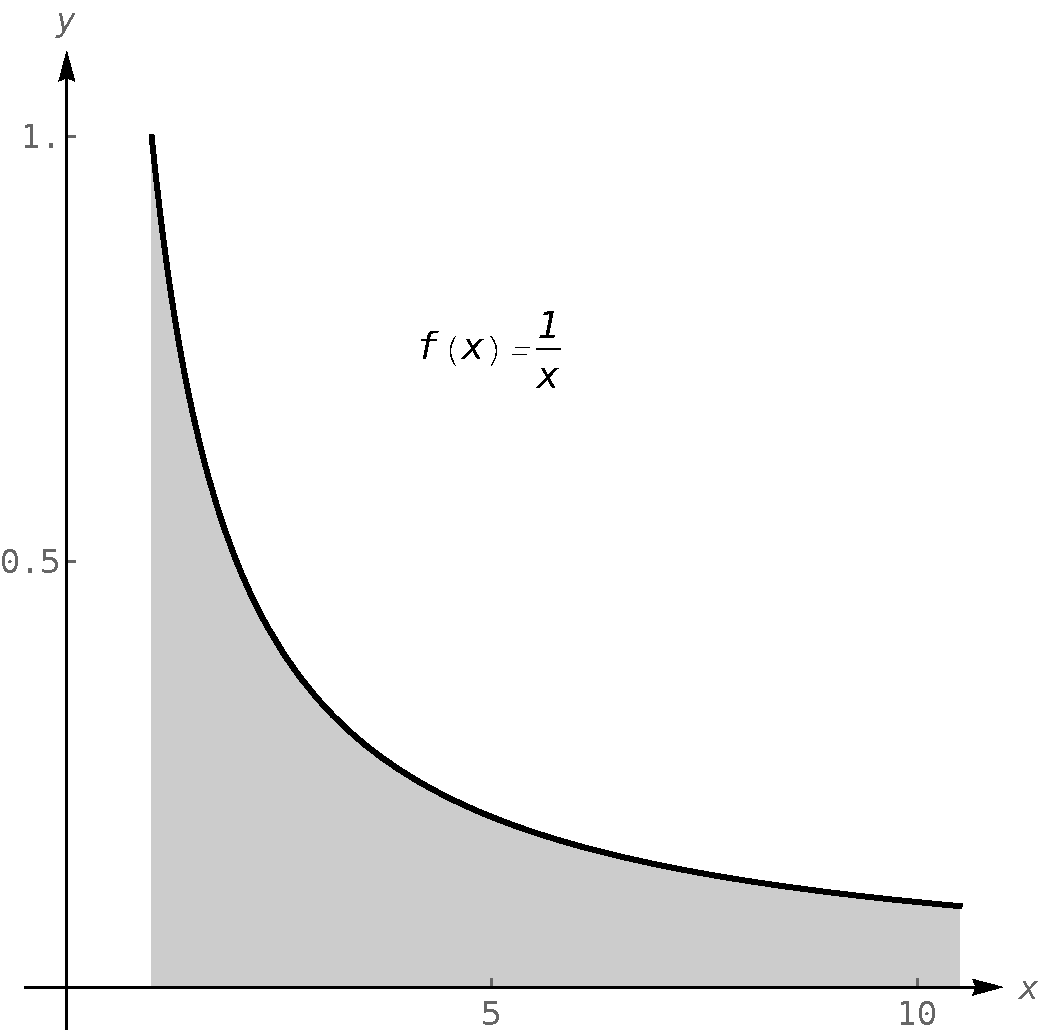
\includegraphics[width=0.3\textwidth]{fig_int_15b} }
\qquad
\subfigure[\label{fig_int_15c}]{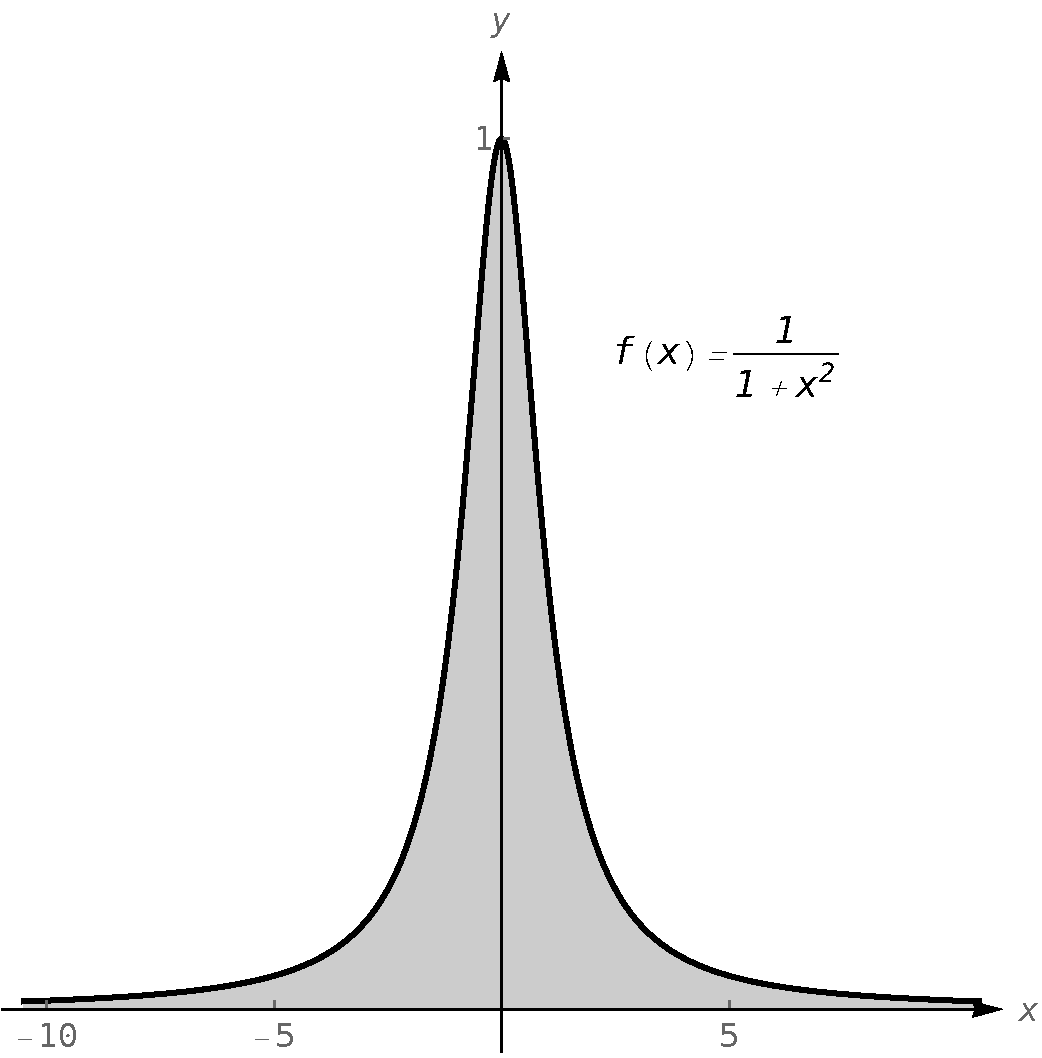
\includegraphics[width=0.3\textwidth]{fig_int_15c} }
\caption{A graph of  $f(x) = \frac{1}{x^2}$ (a),  $f(x) = \frac{1}{x}$ (b) and $f(x) = \frac{1}{1+x^2}$ (c) in Example \ref{ex_impint1}.}
\end{figure} 

\item		We will need to break this into two improper integrals and choose a value of $c$ as in part 3 of Definition \ref{def:imp_int1}. Any value of $c$ is fine; we choose $c=0$.

\begin{align*}%
		\ds \int\limits_{-\infty}^{+\infty} \frac1{1+x^2}\ dx &= \lim_{a\to-\infty} \ds \int\limits_a^0\frac{1}{1+x^2}\ dx + \lim_{b\to+\infty} \ds \int\limits_0^b\frac{1}{1+x^2}\ dx \\[0.2cm]
						&= \lim_{a\to-\infty} \arctan(x)\Big|_a^0 + \lim_{b\to+\infty} \arctan(x)\Big|_0^b\\[0.2cm]
						&= \lim_{a\to-\infty} \left(\arctan(0)-\arctan(a)\right) + \lim_{b\to+\infty} \left(\arctan(b)-\arctan(0)\right)\\[0.2cm]		
						&= \left(0-\frac{-\pi}2\right) + \left(\frac{\pi}2-0\right)\\
						\intertext{Each	limit exists, hence the original integral converges and has value:}
		\ds \int\limits_{-\infty}^{+\infty} \frac1{1+x^2}\ dx &= \pi.
\end{align*}
%\enlargethispage{2\baselineskip}
A graph of the area defined by this integral is given in Figure \ref{fig_int_15c}.



\end{enumerate}
\end{example}

Note that it is not uncommon for the limits resulting from improper integrals to need l'H\^opital's rule.

\subsection{Improper integrals with infinite range}

We have just considered definite integrals where the interval of integration was infinite. We now consider another type of improper integration, where the range of the integrand is infinite.


\begin{definition}[Improper integrals with infinite range]\label{def:imp_int2}
Let $f(x)$ be a continuous function on $[a,b]$ except at $c$, $a\leq c\leq b$, where $x=c$ is a vertical asymptote of $f$. Define\index{integration!improper}\index{improper integration}
$$\ds \int\limits_a^b f(x)\ dx = \lim_{t\underset{<}{\rightarrow}c}\ds \int\limits_a^t f(x)\ dx + \lim_{t\underset{>}{\rightarrow}c}\ds \int\limits_t^b f(x)\ dx.$$
%The integral converges if both limits exist and diverges otherwise.
\end{definition}
\index[aut]{integraal ! oneigenlijk}\index[aut]{oneigenlijke integraal}



\begin{example}\label{ex_impint3}
Evaluate the following improper integrals:
\begin{multicols}{2}
\begin{enumerate}
    \item $\ds \int\limits_0^1\frac1{\sqrt{x}}\ dx, $
    \item $\ds \int\limits_{-1}^1\frac{1}{x^2}\ dx. $
\end{enumerate}
\end{multicols}


\xhrulefill{gray}{2.5pt}Solution \xhrulefill{gray}{2.5pt}


\begin{enumerate}
\item		A graph of $f(x) = 1/\sqrt{x}$ is given in Figure \ref{fig_int_16a}. Notice that $f$ has a vertical asymptote at $x=0$; in some sense, we are trying to compute the area of a region that has no top. Could this have a finite value? 
\begin{align*} \ds \int\limits_0^1 \frac{1}{\sqrt{x}}\ dx &= \lim_{a\underset{>}{\rightarrow}0}\ds \int\limits_a^1 \frac1{\sqrt{x}}\ dx \\[0.2cm]
			&=	\lim_{a\underset{>}{\rightarrow}0} 2\sqrt{x}\Big|_a^1 \\[0.2cm]
			&= \lim_{a\underset{>}{\rightarrow}0} 2\left(\sqrt{1}-\sqrt{a}\right)\\[0.2cm]
			&=	2
\end{align*}
It turns out that the region does have a finite area even though it has no upper bound.


\item		The function $f(x) = 1/x^2$ has a vertical asymptote at $x=0$, as shown in Figure \ref{fig_int_16b}, so this integral is an improper integral. Let's eschew using limits for a moment and proceed without recognizing the improper nature of the integral. This leads to:
\begin{align*}
\ds \int\limits_{-1}^1\frac1{x^2}\ dx &= -\frac1x\Big|_{-1}^1\\[0.2cm]
			&= -1 - (1)\\[0.2cm]
			&=-2. \ (!)
\end{align*}

Clearly the area in question is above the $x$-axis, yet the area is supposedly negative! Why does our answer not match our intuition? To answer this, evaluate the integral using Definition \ref{def:imp_int2}.
\begin{align*}
\ds \int\limits_{-1}^1\frac1{x^2}\ dx &= \lim_{t\underset{<}{\rightarrow}0}\ds \int\limits_{-1}^t \frac1{x^2}\ dx + \lim_{t\underset{>}{\rightarrow}0}\ds \int\limits_t^1\frac1{x^2}\ dx \\[0.2cm]
			&= \lim_{t\underset{<}{\rightarrow}0}\Big(-\frac1x\Big)\Big|_{-1}^t + \lim_{t\underset{>}{\rightarrow}0}\Big(-\frac1x\Big)\Big|_t^1\\[0.2cm]
			&= \lim_{t\underset{<}{\rightarrow}0}\Big(-\frac1t-1\Big) + \lim_{t\underset{>}{\rightarrow}0} \Big(-1+\frac1t\Big)\\[0.2cm]
			&= \Big(+\infty-1\Big)\ + \ \Big(- 1+\infty\Big)
\end{align*}
Neither limit converges hence the original improper integral diverges. The nonsensical answer we obtained by ignoring the improper nature of the integral is just that: nonsensical.

\end{enumerate}
\begin{figure}[H]
\centering
%\raisebox{0.5cm}{
\subfigure[\label{fig_int_16a}]{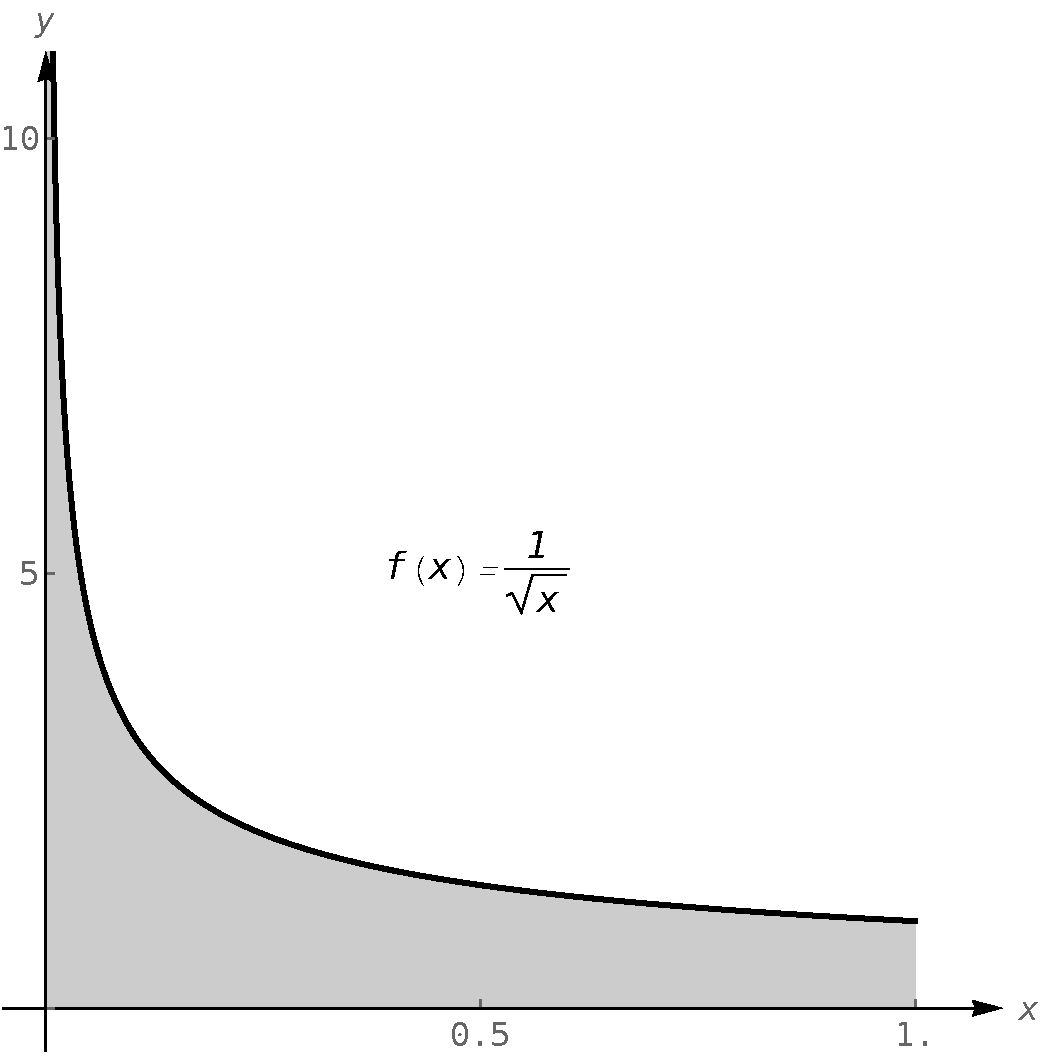
\includegraphics[width=0.3\textwidth]{fig_int_16a}}
\qquad
\subfigure[\label{fig_int_16b}]{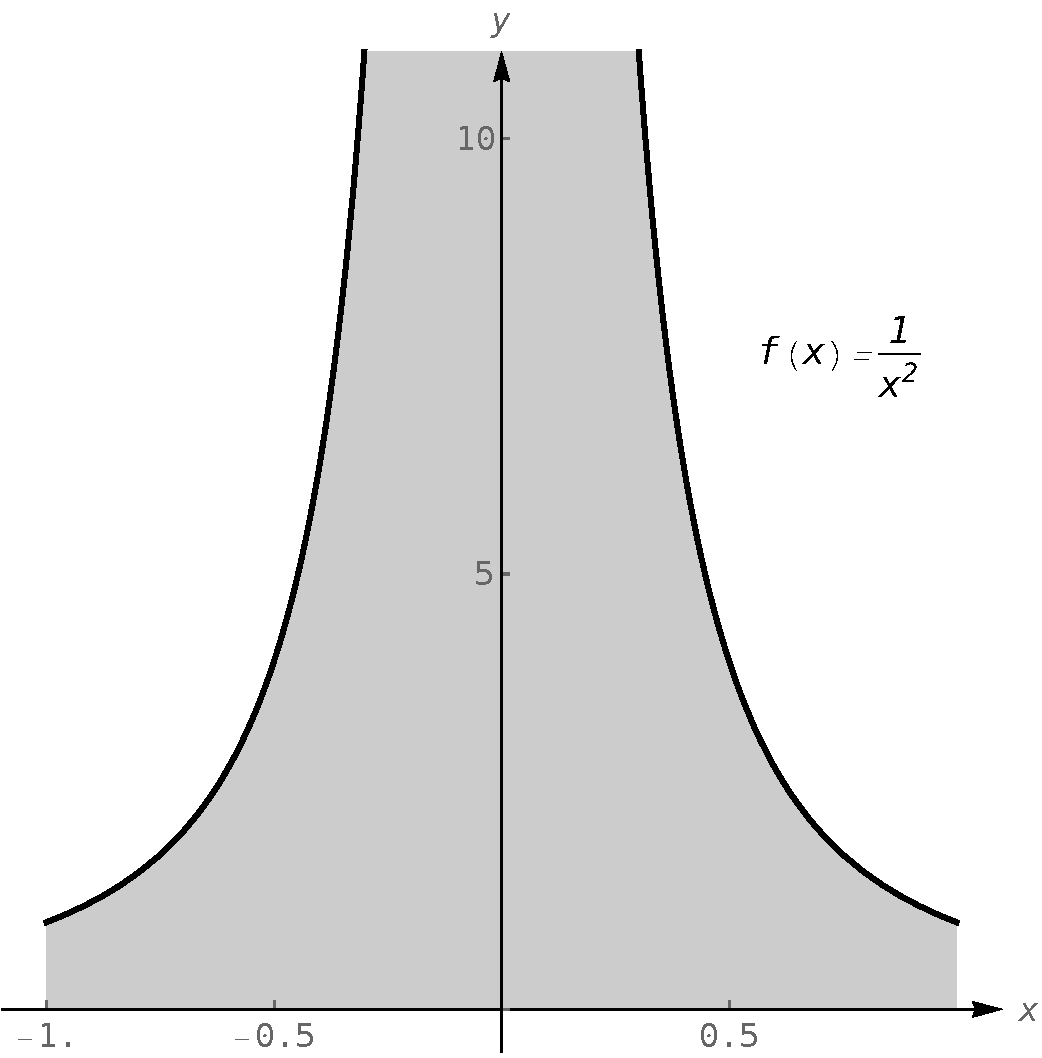
\includegraphics[width=0.3\textwidth]{fig_int_16b} }
\caption{A graph of $f(x)=\frac{1}{\sqrt{x}}$ (a) and $f(x)=\frac{1}{x^2}$ (b)  in Example \ref{ex_impint3}.}
\end{figure} 

\end{example}

\ifanalysis
\subsection{Convergence and divergence}

Oftentimes we are interested in knowing simply whether or not an improper integral converges, and not necessarily the value of a convergent integral. We provide here several tools that help determine the \textbf{convergence} (\textit{convergentie}) or \textbf{divergence} (\textit{divergentie}) of improper integrals without integrating.
\index{convergence} \index{divergence}
\index[aut]{divergentie} \index[aut]{convergentie}

For instance, let us try to determine the values of $p$ for which 
$$\ds \int\limits_1^{+\infty} \frac1{x\hskip1pt ^p}\ dx$$
 converges.

We begin by integrating and then evaluating the limit:
\allowdisplaybreaks
\begin{align*}
\ds \int\limits_1^{+\infty} \frac1{x\hskip1pt ^p}\ dx &=	\lim_{b\to+\infty}\ds \int\limits_1^b\frac1{x\hskip1pt ^p}\ dx\\[0.2cm]
		&=	\lim_{b\to+\infty}\ds \int\limits_1^b x^{-p}\ dx \qquad \text{\small (assume $p\neq 1$)}\\[0.2cm]
		&= \lim_{b\to+\infty} \frac{1}{-p+1}x^{-p+1}\Big|_1^b\\[0.2cm]
		&= \lim_{b\to+\infty} \frac{1}{1-p}\big(b\hskip1pt^{1-p}-1^{1-p}\big).\\[0.2cm]
\end{align*}
When does this limit converge -- i.e., when is this limit not $\infty$? This limit converges precisely when the power of $b$ is less than 0: when $1-p<0 \Rightarrow 1<p$. 


So, if $p>1$, then $\int_1^\infty \frac1{x\hskip1pt ^p}\ dx $ converges. When $p<1$ the improper integral diverges; we showed in Example \ref{ex_impint1} that when $p=1$ the integral also diverges.  Figure \ref{fig_int_17} graphs $y=1/x$ with a dashed line, along with graphs of $y=1/x^p$, $p<1$, and $y=1/x^q$, $q>1$. Somehow the dashed line forms a dividing line between convergence and divergence. 

\begin{figure}
	\begin{center}
			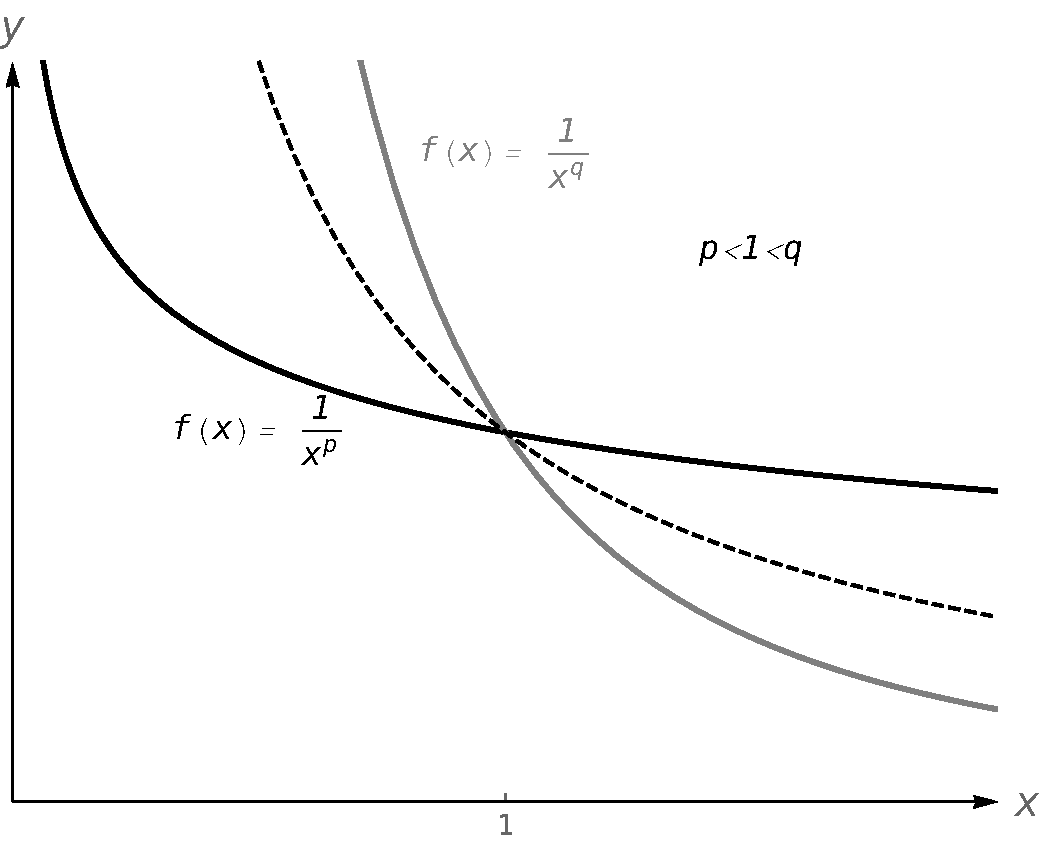
\includegraphics[width=0.5\textwidth]{fig_int_17}
	\caption{Plotting functions of the form $1/x\,^p$.}
	\label{fig_int_17}
	\end{center}
\end{figure}

A similar result is proved in the exercises about improper integrals of the form 
$$\ds \int\limits_0^1\frac1{x\hskip1pt ^p}\ dx,$$
i.e.\ this improper integral  converges when $p<1$ and diverges when $p\geq 1.$


Note that we used the upper and lower bound of 1 just for convenience. It can be replaced by any $a$ where $a>0$. 

A basic technique in determining convergence of improper integrals is to compare an integrand whose convergence is unknown to an integrand whose convergence is known. We often use integrands of the form $1/x\hskip1pt ^p$ to compare to as their convergence on certain intervals is known. This is described in the following theorem.




\begin{theorem}[Direct comparison test for improper integrals]\label{thm:impint_comparison}
%\begin{itemize}
%\item		
Let $f$ and $g$ be continuous on $[a,+\infty\left[\right.$ where $0\leq f(x)\leq g(x)$ for all $x$ in $[a,+\infty\left[\right.$. 
	\begin{enumerate}
	\item		If $\ds \int\limits_a^{+\infty} g(x)\ dx$ converges, then $\ds \ds \int\limits_a^{+\infty} f(x)\ dx$ converges.
	\index{integration!improper}\index{convergence!Direct Comparison Test!for integration}\index{divergence!Direct Comparison Test!for integration}\index{Direct Comparison Test!for integration}\index{convergence!of improper int.}\index{divergence!of improper int.}
	\item		If $\ds \int\limits_a^{+\infty} f(x)\ dx$ diverges, then $\ds \int\limits_a^{+\infty} g(x)\ dx$ diverges.
	\end{enumerate}
	\end{theorem}
	
\ifanalysis

\pagebreak
To prove Theorem~\ref{thm:impint_comparison}, let us first of all prove the following theorem, which will need later on. 
\begin{theorem}[Limit of an increasing function bounded from above]\label{lemma1}
Let $F(t)$ be an increasing function on an interval $\left.\right]a,+\infty\left[\right.$. Assume there exists $M>0$ such that $F(t)\leq M$ for all $t\in \left.\right]a,+\infty\left[\right.$. Then the following limit exists:
$$L=\lim_{t\to+\infty}F(t),$$
and $L\leq M$. 
\end{theorem}

\begin{proof}
Let $S$ be the set of values of $F(t)$ on  $\left.\right]a,+\infty\left[\right.$:
$$
S=\left\{y\mid y=F(t), \; \forall t> a\right\}.
$$
By assumption, $S$ is bounded by $M$ , that is, $y\leq M$ for all $y\in S$, so $S$ has a least upper bound (supremum). Let
$L=\sup(S)$. Then for all $\epsilon>0$, $L-\epsilon$ is not an upper bound for $S$, so there exists some $y_0>a$ such that $F(y_0)>L- \epsilon$. Since $F(t)$ is an increasing function, it follows that
$$
L-\epsilon\leq F(y_0)\leq F(t)\leq L
$$
for $t>y_0$. Therefore, $\left|L-F(t)\right|<\epsilon$ for $t>y_0$. Since $\epsilon$ is an arbitrary positive number, this is
precisely what is needed to conclude that
$$L=\lim_{t\to+\infty}F(t).$$
\phantom{}
\end{proof}

\begin{proof}[of Theorem~\ref{thm:impint_comparison}]
Now to prove the first part of Theorem~\ref{thm:impint_comparison}, consider the functions
$$
G(t)=\ds \int\limits_a^t g(x)\ dx\qquad\text{and}\qquad F(t)=\ds \int\limits_a^t f(x)\ dx
$$
They are defined for $t>a$. Since $f(x)\geq 0$  and $g(x)\geq0$, both $F(t)$ and $G(t)$ are increasing. Furthermore, $f(x)\leq g(x)$ for all $x\geq a$ and therefore,
\begin{equation}
F(t)\leq G(t)
\label{compar_test1}
\end{equation}
for all $t\geq a$.
%Bron: http://bcs.whfreeman.com/webpub/Ektron/rogawskiapet2e/Additional%20Proofs/Proof%20of%20Comparison%20Test%20for%20Improper%20Integrals.pdf


Our assumption now is that the following improper integral converges:
$$
M= \ds \int\limits_a^{+\infty} g(x)\ dx\,.
$$
By definition, we have that $M=\displaystyle\lim_{t\to+\infty}G(t)$. Since $G(t)$ is increasing, it holds that
$$
G(t)\leq M
$$
for all $t\geq a$, and it subsequently follows from Inequality~\eqref{compar_test1} that
$$
F(t)\leq M
$$
for all $t\geq a$.

Since we have shown that $F(t)$ is increasing and bounded by $M$, we can  conclude that $\displaystyle\lim_{t\to+\infty}F(t)$ exists. Since this limit is equal to the desired improper integral
$$
\lim_{t\to+\infty}F(t)=\ds \int\limits_a^{+\infty} f(x)\ dx\,,
$$
this concludes our proof of the first part. Moreover, the second part follows immediately. Indeed,  assume that the
first part is known to be true and that
$$
\ds \int\limits_a^{+\infty} f(x)\ dx
$$
diverges. Then 
$$
\ds \int\limits_a^{+\infty} g(x)\ dx
$$
must diverge as well, for if it converged, the first part would imply that
$$
\ds \int\limits_a^{+\infty} f(x)\ dx
$$
converges. Similarly, the second part implies the first.
\end{proof}

There is also a counterpart of Theorem~\ref{thm:impint_comparison} for improper integrals with infinite range. 

\begin{theorem}[Direct comparison test for improper integrals with infinite range]\label{thm:impint_comparison2}
%\begin{itemize}
%\item		
Let $f$ and $g$ be continuous on $[a,x_0\left[\right.$ where $0\leq f(x)\leq g(x)$ for all $x$ in $[a,x_0\left[\right.$. 
	\begin{enumerate}
	\item		If $\ds \int\limits_a^{x_0} g(x)\ dx$ converges, then $\ds \int\limits_a^{x_0} f(x)\ dx$ converges.
	\index{integration!improper}\index{convergence!Direct Comparison Test!for integration}\index{divergence!Direct Comparison Test!for integration}\index{Direct Comparison Test!for integration}\index{convergence!of improper int.}\index{divergence!of improper int.}
	\item		If $\ds \int\limits_a^{x_0} f(x)\ dx$ diverges, then $\ds \int\limits_a^{x_0} g(x)\ dx$ diverges.
	\end{enumerate}
	\end{theorem}
	

\fi


\begin{example}\label{ex_impint5}
Determine the convergence of the following improper integrals.

%\noindent%
%\begin{minipage}[t]{.5\textwidth}
\begin{multicols}{2}
\begin{enumerate}
\item $ \ds \int\limits_1^{+\infty} e^{-x^2}\ dx$
\item $\ds \int\limits_3^{+\infty} \frac{1}{\sqrt{x^2-x}}\ dx$
\end{enumerate}
\end{multicols}
%\end{minipage}
%\begin{minipage}[t]{.5\textwidth}
%\begin{enumerate}\addtocounter{enumi}{2}
%\item		$\ds \int_0^2\frac{1}{(x+5)^{1/3}}\ dx$
%\end{enumerate}
%\end{minipage}

\xhrulefill{gray}{2.5pt}Solution \xhrulefill{gray}{2.5pt}

\begin{enumerate}
\item		The function $f(x) = e^{-x^2}$ does not have an antiderivative expressible in terms of elementary functions, so we cannot integrate directly. It is comparable to $g(x)=1/x^2$, and as demonstrated in Figure \ref{fig_int_18a}, $e^{-x^2} < 1/x^2$ on $[1,+\infty\left[\right.$. We know that $ \int_1^{+\infty} x^{-2}\ dx$ converges, hence  also the improper integral under consideration converges.

\item		Note that for large values of $x$, we have
$$\ds \frac{1}{\sqrt{x^2-x}} \approx \frac{1}{\sqrt{x^2}} =\frac{1}{x}.$$
We know that  $ \int_3^{+\infty} x^{-1}\ dx$ diverges, so we seek to compare the original integrand to $1/x$. It is easy to see that when $x>0$, we have  $$x = \sqrt{x^2} > \sqrt{x^2-x}\quad\Leftrightarrow\quad\frac1x < \frac1{\sqrt{x^2-x}}.$$

Using Theorem \ref{thm:impint_comparison}, we conclude that since $\int_3^{+\infty}x^{-1}\ dx$ diverges, the concerned improper integral diverges as well. Figure \ref{fig_int_18b} illustrates this.


\end{enumerate}
\begin{figure}[H]
\centering
%\raisebox{0.5cm}{
\subfigure[\label{fig_int_18a}]{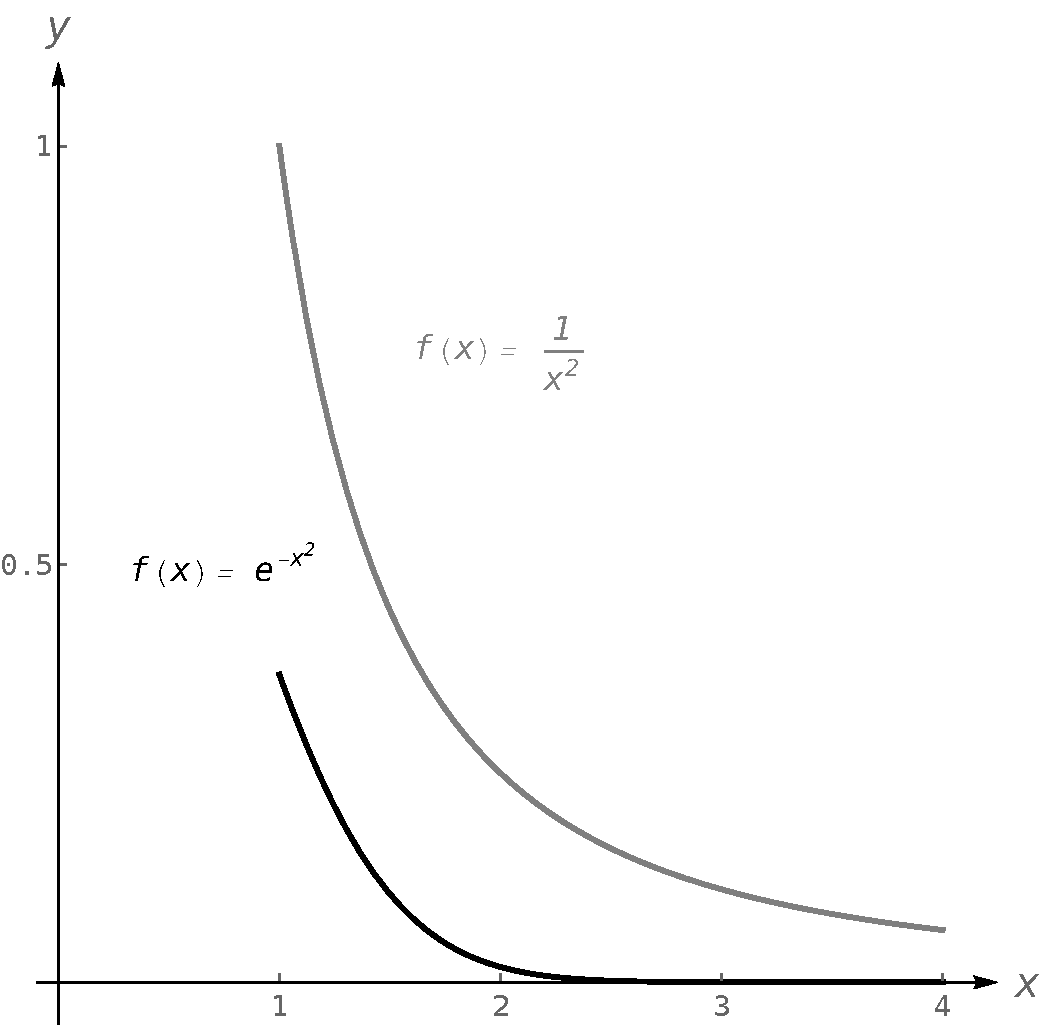
\includegraphics[width=0.45\textwidth]{fig_int_18a}}
\qquad
\subfigure[\label{fig_int_18b}]{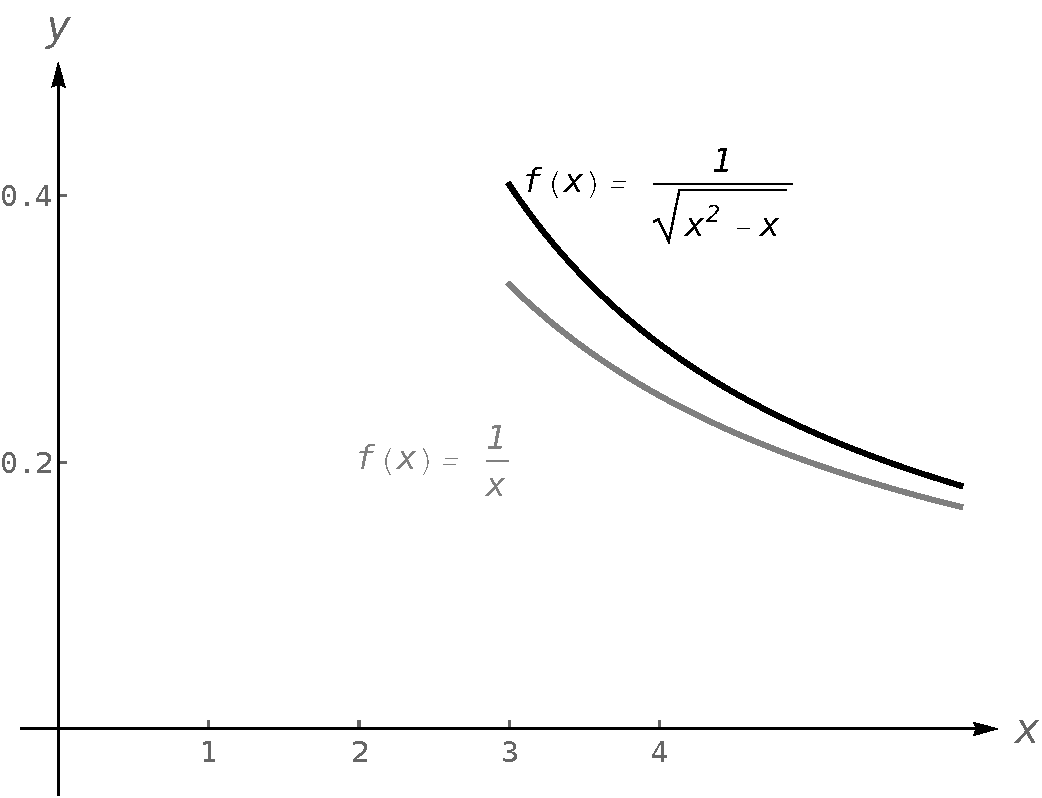
\includegraphics[width=0.45\textwidth]{fig_int_18b} }
\caption{Graphs of $f(x) = e^{-x^2}$ and $f(x)= 1/x^2$ (a) and of $f(x) = 1/\sqrt{x^2-x}$ and $f(x)= 1/x$ (b) in Example \ref{ex_impint5}.}
\end{figure} 
\end{example}


Being able to compare unknown integrals to known integrals is very useful in determining convergence. However, some of our examples were a little too nice. For instance, it was convenient that \linebreak $\frac{1}x < \frac{1}{\sqrt{x^2-x}}$, but what if the $-x$ were replaced with a $+2x+5$? That is, what can we say about the convergence of
$$\ds \int\limits_3^{+\infty}\frac{1}{\sqrt{x^2+2x+5}}\ dx?$$
We have 
$$\ds \frac{1}{x} > \frac1{\sqrt{x^2+2x+5}},$$
so we cannot use Theorem \ref{thm:impint_comparison}.

In cases like this (and many more) it is useful to employ the following theorem.


\begin{theorem}[Limit comparison test for improper integrals]\label{thm:impint_limit}

%\begin{itemize}
		Let $f$ and $g$ be continuous functions on $[a,+\infty\left[\right.$ where $f(x)>0$ and $g(x)>0$ for all $x$. If $$\lim_{x\to+\infty} \frac{f(x)}{g(x)} = L,\qquad 0<L<+\infty,$$
	then 
	$$\ds \int\limits_a^{+\infty} f(x)\ dx \text{ is convergent } \quad \Leftrightarrow \quad  \ds \int\limits_a^{+\infty} g(x)\ dx \text{ is convergent }\,, $$ 
	and equivalently,
	$$\ds \int\limits_a^{+\infty} f(x)\ dx \text{ is divergent } \quad \Leftrightarrow \quad  \ds \int\limits_a^{+\infty} g(x)\ dx \text{ is divergent }\,. $$ 
	%
\index{convergence!limit comparison test }\index{divergence!limit comparison test}\index{limit comparison test}\index{convergence}\index{divergence}
%	\item		Let $f$ and $g$ be continuous functions on $[a,b]$ except at $x=c$, where each has a vertical asymptote, and $f(x)>0$ and $g(x)>0$ for all $x$ in $[a,b]$, $x\neq c$. If
%	$$\lim_{x\to c^-} \frac{f(x)}{g(x)} = L_1 \quad \text{and} \quad \lim_{x\to c^+}\frac{f(x)}{g(x)} = L_2,\qquad 0<L_1,L_2<\infty,$$
%	then $$\int_a^b f(x)\ dx \quad \text{and} \quad \int_a^b g(x)\ dx$$ either both converge or both diverge.
%\end{itemize}
\end{theorem}

\ifanalysis

\begin{proof}
We assume that $L$ exists and is a positive finite number, and that the limit from $a$ to $+\infty$ of $g$ converges; we will show that the limit from $a$ to $+\infty$ of $f$ converges as well. 

The definition of the limit tells us that, given the number $\epsilon=L/2$, there exists some $M$ such that
$$
\frac{L}{2}=L-\epsilon< \frac{f(x)}{g(x)}<L+\epsilon=\frac{3L}{2}
$$
whenever $x>M$. So, for those values of $x$, we have that 

\begin{equation}
\frac{L}{2}g(x)<f(x)<\frac{3L}{2}g(x)\,.
\label{compar_test2}
\end{equation}
Let us now break the following integral in question into two pieces:
$$
\ds \int\limits_a^{+\infty} f(x)\ dx=\ds \int\limits_a^{M} f(x)\ dx+\ds \int\limits_{M}^{+\infty} f(x)\ dx.
$$
The first integral is of a continuous function on a closed, bounded interval, so we know that is finite. The convergence of the second integral is concluded by the following, which we can do because of Inequality~\eqref{compar_test2}:
$$
\ds \int\limits_{M}^{+\infty} f(x)\ dx<\frac{3L}{2}\ds \int\limits_{M}^{+\infty} g(x)\ dx.
$$
the last integral in this equation is given to converge (our assumption); therefore, by Theorem~\ref{thm:impint_comparison}, the integral on the left converges as well. Hence, we conclude, as desired, that the integral of $f$ converges. 

Proving the other direction can be done similarly, or simply by observing that if $\lim\limits_{x \to +\infty}\frac{f(x)}{g(x)}=k$ exists and is positive, then
$\lim\limits_{x \to +\infty}\frac{g(x)}{f(x)}=\frac{1}{k}$ must also exist and be positive.
\end{proof}

%Bron: https://www.math.toronto.edu/mat137/files/137_LCT2.pdf

The limit comparison test can as well be given for unproper integrals with an infinite range.


\pagebreak
\begin{theorem}[Limit comparison test for improper integrals with infinite range]\label{thm:impint_limit2}

%\begin{itemize}
		Let $f$ and $g$ be continuous functions on $[a,{x_0}\left[\right.$ where $f(x)>0$ and $g(x)>0$ for all $x$. If $$\lim_{x\to x_0} \frac{f(x)}{g(x)} = L,\qquad 0<L<\infty,$$
	then 
	$$\ds \int\limits_a^{x_0} f(x)\ dx \text{ is convergent }\Leftrightarrow  \ds \int\limits_a^{x_0} g(x)\ dx \text{ is convergent,} $$ 
	and equivalently,
	$$\ds \int\limits_a^{x_0} f(x)\ dx \text{ is divergent }\Leftrightarrow  \ds \int\limits_a^{x_0} g(x)\ dx \text{ is divergent.} $$ 
	%Bron: http://www-personal.umich.edu/~tghyde/LimitComparison.pdf
\index{convergence!limit comparison test }\index{divergence!limit comparison test}\index{limit comparison test}\index{convergence}\index{divergence}
%	\item		Let $f$ and $g$ be continuous functions on $[a,b]$ except at $x=c$, where each has a vertical asymptote, and $f(x)>0$ and $g(x)>0$ for all $x$ in $[a,b]$, $x\neq c$. If
%	$$\lim_{x\to c^-} \frac{f(x)}{g(x)} = L_1 \quad \text{and} \quad \lim_{x\to c^+}\frac{f(x)}{g(x)} = L_2,\qquad 0<L_1,L_2<\infty,$$
%	then $$\int_a^b f(x)\ dx \quad \text{and} \quad \int_a^b g(x)\ dx$$ either both converge or both diverge.
%\end{itemize}
\end{theorem}

\fi


\begin{example}\label{ex_impint6}
Determine the convergence of 
$$\ds \int\limits_3^{+\infty} \frac{1}{\sqrt{x^2+2x+5}}\ dx.$$

\xhrulefill{gray}{2.5pt}Solution \xhrulefill{gray}{2.5pt}

As $x$ gets large, the denominator of the integrand will begin to behave much like $y=x$. So we compare 
$$\ds\frac{1}{\sqrt{x^2+2x+5}}$$ to $1/x$ using Theorem~\ref{thm:impint_limit}:

$$
\lim_{x\to+\infty} \frac{1/\sqrt{x^2+2x+5}}{1/x} = \lim_{x\to+\infty}\frac{x}{\sqrt{x^2+2x+5}}.$$

The immediate evaluation of this limit returns $\infty/\infty$, an indeterminate form. Using l'H\^opital's rule seems appropriate, but in this situation, it does not lead to useful results. 

The trouble is the square root function. To get rid of it, we employ the following fact: If $\ds \lim_{x\to c} f(x) = L$, then $\ds\lim_{x\to c} f(x)^2 = L^2.$  So we consider now the limit
$$\lim_{x\to+\infty} \frac{x^2}{x^2+2x+5}.$$ This converges to 1, meaning the original limit also converged to 1. As $x$ gets very large, the function 
\small$\ds\frac{1}{\sqrt{x^2+2x+5}}$\normalsize\ looks very much like \small$\ds\frac1x.$\normalsize\ 
Since we know that 
$$\ds \int\limits_3^{+\infty} \frac1x\ dx$$\normalsize\ diverges, by Theorem~\ref{thm:impint_limit} we know that 
$$\ds \int\limits_3^{+\infty}\frac{1}{\sqrt{x^2+2x+5}}\ dx$$
\normalsize also diverges. Figure \ref{fig_int_19} graphs $f(x)=1/\sqrt{x^2+2x+5}$ and $f(x)=1/x$, illustrating that as $x$ gets large, the functions become indistinguishable.

\begin{figure}[H]
	\begin{center}
			\includegraphics[width=0.45\textwidth]{fig_int_19}
	\caption{Graphing $f(x)=\frac{1}{\sqrt{x^2+2x+5}}$ and $f(x)=\frac1x$ in Example \ref{ex_impint6}.}
	\label{fig_int_19}
	\end{center}
\end{figure}


\end{example}

%\enlargethispage{3\baselineskip}

\fi

\ifmathematica
This chapter has explored many integration techniques.  All of them effectively have one goal in common: rewrite the integrand in a new way so that the integration step is easier to see and implement. As stated before, integration is, in general, hard. It is easy to write a function whose antiderivative is impossible to write in terms of elementary functions, and even when a function does have an antiderivative expressible by elementary functions, it may be really hard to discover what it is. Mathematica, for instance, has approximately 1,000 pages of code dedicated to integration. Do not let this difficulty discourage you. There is great value in learning integration techniques, as they allow one to manipulate an integral in ways that can illuminate a concept for greater understanding. There is also great value in understanding the need for good numerical techniques.
\fi
\ifpython
This chapter has explored many integration techniques.  All of them effectively have one goal in common: rewrite the integrand in a new way so that the integration step is easier to see and implement. As stated before, integration is, in general, hard. It is easy to write a function whose antiderivative is impossible to write in terms of elementary functions, and even when a function does have an antiderivative expressible by elementary functions, it may be really hard to discover what it is. Python, for instance, has approximately 1,000 pages of code dedicated to integration. Do not let this difficulty discourage you. There is great value in learning integration techniques, as they allow one to manipulate an integral in ways that can illuminate a concept for greater understanding. There is also great value in understanding the need for good numerical techniques.
\fi
The next chapter stresses the uses of integration. We generally do not find antiderivatives for antiderivative's sake, but rather because they provide the solution to some type of problem. The following chapter introduces us to a number of different problems whose solution is provided by integration.


 
\newpage
\section{Exercises}
\subsection{Analytical exercises}

\renewcommand{\ExerciseListName}{Assignements}

\subsection*{\nameref{sec:antider}}
%%%%%%%%%%%%%%%%%%%
%Oefening 4 Bio-irs
%Oefening 1 Ings
%%%%%%%%%%%%%%%%%%%
\ifanalysis\begin{Exercise}[difficulty = 1]\fi\ifcalculus\begin{Exercise}[difficulty = 2]\fi
Determine the area between the $x$-axis and the graph of the function:
\[
f(x) = \left\{\begin{array}{lcl}
x,  & \text{ als  } & 0<x\leq1\,,\\[0.1cm]
-2x+3,  & \text{ als  } & 1<x\leq2\,,\\[0.1cm]
-1,   & \text{ als  } &  2<x\leq3\,,\\[0.1cm]
0,   & \text{ als  } &  x \leq 0 \,  \vee \, x > 3\,.
\end{array}\right.
\]

\ifanalysis\end{Exercise}\fi\ifcalculus\end{Exercise}\fi
\setboolean{firstanswerofthechapter}{true}
\begin{Answer}\phantom{}
    The area is $2$.
\end{Answer}
\setboolean{firstanswerofthechapter}{false}


\ifanalysis
\subsection*{\nameref{sec:riemann}}
%%%%%%%%%%%%%%%%%%%
%Oefening 1 Bio-irs
%%%%%%%%%%%%%%%%%%%

\begin{Exercise}
Consider a partition of the interval $[a,b]$ in $n$ subintervals of equal width $\Delta x_i = (b-a)/n$. Determine the upper and lower Riemann sum for the given functions and $n$.
\begin{multicols}{2}
	\Question[difficulty = 1] $f(x)=x$, \quad $[0,2]$, \quad $n=8$
	\Question[difficulty = 1] $f(x)=\ln (x)$, \quad $[1,2]$, \quad $n=5$
	\Question[difficulty = 1] $f(x)=\sin (x)$, \quad $[0,\pi]$, \quad $n=6$
	\ifanalysis\Question[difficulty = 1]\fi\ifcalculus\Question[difficulty = 2]\fi $f(x)=\cos (x)$, \quad $[0,2\pi]$, \quad $n=4$
	\Question[difficulty = 1] $f(x)=x^2$, \quad $[-3,3]$, \quad $n=6$ 
	\ifanalysis\Question[difficulty = 1]\fi\ifcalculus\Question[difficulty = 2]\fi $f(x)=\dfrac{1}{x}$, \quad $[1,9]$, \quad $n=4$ 
	\EndCurrentQuestion
\end{multicols}
\end{Exercise}
%\setboolean{firstanswerofthechapter}{true}
\begin{Answer} \phantom{}
    
    \Question $S_l(8) = \dfrac{7}{4}; \quad S_u(8) = \dfrac{9}{4}$ 
    \Question $S_l(5) = 0,3153168; \quad S_u(5) = 0,4539462$ 
    \Question $S_l(6) = 1,43; \quad S_u(6) = 2,48$ 
    \Question $S_l(4) = -\pi; \quad S_u(4)  = \pi$ 
    \Question $S_l(6) = 10; \quad S_u(6)  = 28$ 
    \Question $S_l(4) = \dfrac{496}{315}; \quad S_u(4)  = \dfrac{4352}{105}$
 
\end{Answer}
%\setboolean{firstanswerofthechapter}{false}

%%%%%%%%%%%%%%%%%%%
%Oefening 2 Bio-irs
%%%%%%%%%%%%%%%%%%%
\begin{Exercise}
Express the given limit as a definite integral.
%\begin{multicols}{2}
	\Question[difficulty = 2]  $\dlim_{n \rightarrow +\infty} \,\sum_{i=1}^n \dfrac{1}{n} \sqrt{\frac{i}{n}}$
	\Question[difficulty = 2]  $\dlim_{n \rightarrow +\infty} \, \sum_{i=1}^n \dfrac{1}{n} \sqrt{\frac{i-1}{n}}$
	\Question[difficulty = 2]  $\dlim_{n \rightarrow +\infty} \, \sum_{i=1}^n \dfrac{2}{n} \ln\left(1+{\frac{2i}{n}}\right)$
%\end{multicols}
\end{Exercise}

\begin{Answer}
    \begin{multicols}{3}
    
    \Question $\ds \int\limits_0^1 \sqrt{x}\, dx$
    \Question $\ds \int\limits_0^1 \sqrt{x}\, dx$
    \Question $\ds \int\limits_0^2 \ln(1+x)\, dx$
   \EndCurrentQuestion
    \end{multicols}
\end{Answer}

\fi


\subsection*{\nameref{sec:FTC}}
\ifanalysis
%%%%%%%%%%%%%%%%%%%
%Oefening 3 Bio-irs
%%%%%%%%%%%%%%%%%%%
\ifanalysis\begin{Exercise}[difficulty = 1]\fi\ifcalculus\begin{Exercise}[difficulty = 2]\fi
If $a<b$ and $f$ is continuous over $[a,b]$, prove that
\[ \ds \int\limits_a^b \left(f(x)- \bar{f} \right) dx=0,  \] 
with $\bar{f}$ being the mean of $f$.

\ifanalysis\end{Exercise}\fi\ifcalculus\end{Exercise}\fi

\begin{Answer}
    $\bar{f}$ is the mean  of $f$. %Use definition 12.5 to prove equivalence.
\end{Answer}
\fi


%%%%%%%%%%%%%%%%%%%
%Oefening 7 Bio-irs
%Oefening 2 Ings
%%%%%%%%%%%%%%%%%%%
\begin{Exercise}
Find the derivative of the functions below. 	\begin{multicols}{2}
		\Question[difficulty = 1] $F(x) = \ds \int\limits_2^{x^3+x} \dfrac{1}{t}\, dt$ 
		\Question[difficulty = 1] $F(x) = \ds \int\limits_{x^3}^0 t^3\, dt$ %Apex oef 5.4.54
		\Question[difficulty = 1] $F(t) = \ds \int\limits_{-\pi}^t\dfrac{\cos (y)}{1+y^2}\, dy$
		\Question[difficulty = 1] $F(t) = \ds \int\limits_t^3\dfrac{\sin (x)}{x}\, dx$
		\ifanalysis\Question[difficulty = 1]\fi\ifcalculus\Question[difficulty = 2]\fi $F(x) = x^2 \ds \int\limits_0^{x^2}\dfrac{\sin (u)}{u}\, du $
		\Question[difficulty = 1] $F(\theta) = \ds \int\limits_{\sin (\theta)}^{\cos (\theta)}\dfrac{dx}{1-x^2}$
		\ifanalysis\Question[difficulty = 1]\fi\ifcalculus\Question[difficulty = 2]\fi $F(x) = 3x \ds \int\limits_4^{x^2} e^{-\sqrt{t}}\, dt $
		\Question[difficulty = 1] $F(x) = \ds \int\limits_{x}^{x^2} (t+2)\, dt$ 
		\Question[difficulty = 1] $F(x) = \ds \int\limits_{\ln(x)}^{e^x} \sin(t)\, dt$
		\EndCurrentQuestion
	\end{multicols}
\end{Exercise}

\begin{Answer}
   
    \begin{multicols}{2}
    	\Question $F'(x)= \dfrac{3x^2+1}{x^3+x}$ 
    	\Question $F'(x)= -3x^{11}$ 
    	\Question $F'(t)=\dfrac{\cos (t)}{1+t^2}$
    	\Question $F'(t)=-\dfrac{\sin (t)}{t}$
    	\Question $F'(x)=2x \ds \int\limits_0^{x^2}\dfrac{\sin (u)}{u}\, du + 2x \sin (x^2)$
    	\Question $F'(\theta)=-\dfrac{1}{\sin(\theta)} - \dfrac{1}{\cos(\theta)}$
    	\Question $F'(x)=3 \ds \int\limits_4^{x^2} e^{-\sqrt{t}}\, dt  + 6x^2e^{-|x|}$
    	\Question $F'(x) = 2x^3+3x-2$ 
    	\Question $F'(x) =  e^x\sin\left(e^x\right) - \dfrac{\sin \left( \ln (x) \right)}{x}$ 
    	 \EndCurrentQuestion
    \end{multicols}
\end{Answer}

\ifcalculus \pagebreak \fi
\subsection*{\nameref{sec:techniques_of_antidifferentiation}}
%%%%%%%%%%%%%%%%%%%
%Oefening 4 Ings
%%%%%%%%%%%%%%%%%%%	
\ifcalculus
\begin{Exercise} Determine the integrals below 
	\begin{multicols}{2}
	\Question[difficulty = 1] $\ds \int (1-x)\,\sqrt{x}\; dx$
	\Question[difficulty = 1] $\ds \int \left(4x^3-7x+5\right) dx$
	\Question[difficulty = 1] $\ds \int \left(3x^3+2\sin(x)\right) dx$
	\Question[difficulty = 1] $\ds \int \left(2x^3+3x-1\right)^{1/3}\left(2x^2+1\right) dx$
	\Question[difficulty = 1] $\ds \int \sin(x)\cos(3x)\; dx$
	\Question[difficulty = 1] $\ds \int \sin(6x)\sin(4x)\; dx$
	\Question[difficulty = 1] $\ds \int 2x \ln(x+1) \; dx $ %Uit Van Hecke H10, vb 10.5
	\Question[difficulty = 1] $\ds \int\dfrac{1}{x^2(x+1)}\; dx $
	\Question[difficulty = 1] $\ds \int\dfrac{dx}{\sqrt{-x^2+2x+3}} $ %Uit Van Hecke H10, vb 10.6
	\Question[difficulty = 1] $\ds \int\dfrac{2x+1}{-x^2+3x+2}\; dx $ %Uit Van Hecke H10, vb 10.7
	\Question[difficulty = 1] $\ds \int \dfrac{\sin(x)}{1-\cos(x)}\; dx$
	\Question[difficulty = 1] $\ds \int \dfrac{dx}{4+x^2}$
	\Question[difficulty = 1] $\ds \int x\sin(x)\; dx$
	\Question[difficulty = 1] $\ds \int (x+1)^2\cos(2x)\; dx$
	\Question[difficulty = 1] $\ds \int e^{-x}\sin(2x)\; dx$
	\Question[difficulty = 1] $\ds \int x^n\ln(x)\; dx$
	\Question[difficulty = 2] $\ds \int \dfrac{x}{x^2+4x+5}\; dx$
    \EndCurrentQuestion
	\end{multicols}
\end{Exercise}

\begin{Answer}

    \Question $I = \dfrac{2}{3}x^{3/2} - \dfrac{2}{5}x^{5/2} + C$
    
     Can be integrated directly after rewriting $\sqrt{x}$ as $x^{1/2}$ and splitting the integral into the difference of two integrals. 
    \Question $I = x^4-\dfrac{7}{2}x^2+5x+C$
    \Question $I = 3\dfrac{x^4}{4}-2\cos(x)+C$
    \Question $I = \dfrac{1}{4}\left(2x^3+3x-1\right)^{4/3} + C$
    
     Perform the substitution $u=2x^3+3x-1$.
    \Question $I = -\dfrac{1}{8}\cos(4x) + \dfrac{1}{4}\cos(2x) + C$
    
     The integrand can be rewritten as $\sin(x)\cos(3x) = \dfrac{1}{2} (\sin(4x)-\sin(2x))$.
    \Question $I = \dfrac{1}{4}\sin(2x) - \dfrac{1}{20}\sin(10x) + C$ 
    
     The integrand can be rewritten as $\sin(6x)\sin(4x) = \dfrac{1}{2} (\cos(2x)-\cos(10x))$.
    
    \Question  $I =x^2 \ln(x+1) - \dfrac{1}{2}x^2 + x - \ln|x+1| + C$
   
    Perform integration by parts. You obtain an integral of a rational function. Perform Euclidean division and obtain two basic integrals.
    
    \Question $I=-\ln|x|-\dfrac{1}{x}+\ln|x+1|+C$ 
    
     Split the integrand into partial fractions to obtain three basic integrals.
    
    
    \Question $I=\arcsin \left(\dfrac{x-1}{2}\right) + C$
    
     Write the argument of the square root as a perfect square and then set $x-1$ equal to $t$.
    
    
    \Question $I= -\ln |x^2 - 3x - 2| - \dfrac{4}{\sqrt{17}} \ln \left| \dfrac{2x-3 - \sqrt{17}}{2x-3 + \sqrt{17}} \right|  + C$
    
     Rewrite the numerator as the derivative of the denominator. After this you obtain a basic integral and an integral of a rational function. Rewrite the denominator as a perfect square and again obtain a basic integral.
    
    \Question $I = \ln(1-\cos(x)) + C$
    
     Perform the substitution $u=1-\cos(x)$.
    \Question $I = \dfrac{1}{2}\arctan\left(\dfrac{x}{2}\right)$
    
     Perform the substitution $x=2\tan(t)$ or rewrite the denominator as $4(1+(x/2)^2)$. 
    \Question $I = -x\cos(x) + \sin(x) + C$
    
     TUse integration by parts with $u(x)=x$ and $dv(x) = \sin(x)\,dx$.
    \Question $I = \dfrac{1}{2}(x+1)^2\sin(2x) + \dfrac{1}{2}(x+1)\cos(2x) - \dfrac{1}{4}\sin(2x) + C$
    
     Use integration by parts twice, with respectively $u(x)=(x+1)^2$ and $u(x)=x+1$ and with respectively $dv(x)=\cos(2x)\,dx$ and $dv(x)=\sin(2x)\,dx$. 
    \Question $I = -\dfrac{1}{5}e^{-x}\sin(2x) -\dfrac{2}{5}e^{-x}\cos(2x) + C$
    
    Use integration by parts twice with $u(x)=e^(-x)$ and form the equality to determine the integral.
    \Question $I=\dfrac{x^{n+1}\ln(x)}{n+1} - \dfrac{x^{n+1}}{(n+1)^2} + C$
    
     Perform integration by parts with $u(x)=\ln(x)$ and $dv(x)=x^n\,dx$.
    \Question $I = \dfrac{1}{2}\ln\left|x^2+4x+5\right| - 2\arctan(x+2) + C$
   
    Rewrite the statement as follows:
    \[ \ds \int \dfrac{x}{x^2+4x+5}\; dx = \ds \int \dfrac{x+2}{x^2+4x+5}\; dx - 2 \ds \int \dfrac{1}{x^2+4x+5}\; dx.\]
    For the first integral, use the substitution $u=x^2+4x+5$ and rewrite the denominator as $x^2+4x+5=(x+2)^2+1$ in the second integral.

\end{Answer}
\fi	
%%%%%%%%%%%%%%%%%%%
%Oefening 9 Bio-irs
%Oefening 5 Ings
%%%%%%%%%%%%%%%%%%%	

\begin{Exercise} Find the following indefinite integrals.
	\begin{multicols}{2}
		\Question[difficulty = 1] $\ds \int \dfrac{e^x \sqrt{1-x^2}-1}{\sqrt{1-x^2}}\; dx $
		\Question[difficulty = 1] $\ds \int\dfrac{2x+1}{4x^2+4x+3}\; dx $
		\Question[difficulty = 1] $\ds \int\dfrac{\sin (x)}{\cos^6 (x)} \; dx $
		%\Question $\dint\tan^{-1} x\; dx$
		%\Question $\dint e^{2x}\sin 4x\; dx $
		\ifanalysis\Question[difficulty = 1]\fi\ifcalculus\Question[difficulty = 2]\fi$\ds \int \cos^5 (x)\; dx$
		\Question[difficulty = 1] $\ds \int \dfrac{\sin (x) - \cos (x)}{\sin (x) + \cos (x)}\; dx$
		%\Question $\dint\cos\left(\ln x\right)\; dx$
		\Question[difficulty = 1] $\ds \int \dfrac{dx}{\cos^2 (x)\ \sqrt{1-4\tan^2 (x)}}$
		%\Question $\dint \sin^4 x\cos ^2 x\; dx$
		\Question[difficulty = 2] $\ds \int\dfrac{dx}{\left(\cos (x)+\sin (x)\right)^2}$
		\Question[difficulty = 1] $\ds \int\ln\left(x+\sqrt{x^2+5}\right)\;dx$
		%\Question $\dint x^3\sin x\; dx$
		\Question[difficulty = 1] $\ds \int \dfrac{2x-1}{x^2+x-6}\; dx$ 
		\Question[difficulty = 2] $\ds \int \left(\dfrac{x-1}{x^2-5x+6}\right)^2\; dx$ 
		\Question[difficulty = 1] $\ds \int \dfrac{x^2+1}{x^2+2x+2}\; dx$
		\ifanalysis\Question[difficulty = 1]\fi\ifcalculus\Question[difficulty = 2]\fi $\ds \int\dfrac{x+1}{\left(x^2+1\right)^{3/2}}\;dx$
		\Question[difficulty = 2] $\ds \int\dfrac{dx}{\sqrt{4x-x^2}}$
		\ifanalysis\Question[difficulty = 1]\fi\ifcalculus\Question[difficulty = 2]\fi $\ds \int e^{2x} \sin (4x) \; dx$
		\Question[difficulty = 2] $\ds \int \sin^4(x) \cos^2(x)  \; dx$ %vb 12.21 cos^4(x) sin^2(x)
		\Question[difficulty = 2] $\ds \int \dfrac{\cos(x)}{2\cos^2(x) + \sin(x) -1}\ dx$
		\Question[difficulty = 2] $\ds \int \dfrac{dx}{\sin^2(x) \cos^4(x)}$
    	\ifanalysis
    		\Question[difficulty = 2] $\ds \int \dfrac{dx}{\sinh(x)}$
    		\Question[difficulty = 2] $\ds \int \tanh^3 (x) \; dx$
    	\fi
    	\EndCurrentQuestion
		\end{multicols}
\end{Exercise}

\begin{Answer}

    	\Question $I=e^x-\arcsin (x) + C$
    	
    	 Split the integral to obtain two basic integrals.
    	\Question $I=\dfrac{1}{4} \ln \left(4x^2+4x+3\right) + C$
    	
    	 Substitute $4x^2+4x+3$ by $t$.
    	\Question $I=\dfrac{1}{5\cos^5 (x)} + C$
    	
    	 Substitute $\cos(x)$ by $t$.
        %\Question $I=x\tan^{-1} x - \dfrac{1}{2}\ln\left(1+x^2\right) + C$
        %\Question $I=-\dfrac{e^{2x}\cos 4x}{5} + \dfrac{e^{2x}\sin 4x}{10} + C$
    	\Question $ I = \sin (x)- \dfrac{2}{3}\sin^3 (x) + \dfrac{1}{5}\sin^5 (x) + C$
    	
    	 Rewrite the integrand as $\left(\cos^2 (x)\right)^2\cos (x)$ and then use the Pythagorean identity $\cos^2 (x) = 1 - \sin^2 (x)$. Assume $t=\sin (x)$, expand the product and split the integral.
    	\Question $I = -\ln |\sin (x) + \cos (x)| + C $
    	
    	 Use $t=\sin (x)+\cos (x)$.
    		\Question $I = \dfrac{1}{2}\arcsin\left(2\tan (x) \right) + C$
    	
    	 Use $t=2\tan (x)$.
    		
    	\Question $ I = -\dfrac{1}{1+\tan (x)} + C$
    	
    	 Rewrite the denominator by using $(\cos (x) + \sin (x))^2  = \cos^2 (x) \left(1+\tan (x)\right)^2$ and then use $t=1+\tan (x)$.
    	\Question $I = x\ln \left(x+\sqrt{x^2+5}\right) - \sqrt{x^2+5} + C$
    	
    	 Use integration by parts with $u(x) = \ln\left(x+\sqrt{x^2+5}\right)$ and $dv(x)=dx$. Then, use $t^2=x^2+5$.
        
    	\Question $I = \dfrac{3}{5} \ln |x-2| + \dfrac{7}{5} \ln |x+3| + C$ 
    	
    	 Split the integrand into partial fractions.
    	\Question $I = 4\ln |x-2| - \dfrac{1}{x-2} - 4\ln |x-3| - \dfrac{4}{x-3} + C$ 
    	
    	 There are two ways to start. Either you first take the square of the integrand (square of the numerator over square of the denominator) and split the expression into partial fractions, or you first split the  $\dfrac{x-1}{x^2 -5x +6} $ into partial fractions and then square the result. 
    	
    	\Question $I = x - \ln (x^2+2x+2) + \arctan (x+1) + C$
    	
    	 First, perform Euclidean division. Rewrite the numerator of the integral as $2x + 2 - 1$ and split it into two integrals. One integral can be found using $x^2 + 2x + 2=t$. The denominator of the second integral should be written as a perfect square to obtain $\dfrac{1}{1+u^2}$ as integrand. 
    
    	\Question $I = \dfrac{x-1}{\sqrt{1+x^2}} + C$
    
     The denominator contains the square root of the sum of two squares, therefore use \\ $x = \tan (t)$\ifanalysis or $x=\sinh(t)$\fi.
    	
    	\Question $I = \arcsin \left(\dfrac{x-2}{2}\right) + C$
    	
    	 Write the denominator as the square root of the difference of two squares by completing to a perfect square. Then work toward the  integral with integrand $\dfrac{1}{\sqrt{1-u^2}}$ or use $x-2 = 2 \sin (t)$.
    	
    	\Question $I = -\dfrac{e^{2x} \cos (4x)}{5} +  \dfrac{e^{2x} \sin (4x)}{10} + C$
    	
    	 By applying integration by parts twice with $u(x) = e^{2x}$ (choice) you arrive at the original integral $I$. Solve the resulting integral equation for $I$. 
    	
    	\Question $I= \dfrac{1}{16}\left( x - \dfrac{\sin (4x)}{4} - \dfrac{\sin^3 (2x)}{3} \right) + C $ 
        
        Use the angle doubling formula for $\cos (2x)$:
        \[ \sin^2 (x) = \dfrac{1-\cos (2x)}{2}\hspace{1cm}\mbox{en}\hspace{1cm} \cos^2 (x) = \dfrac{1+\cos (2x)}{2}.\]
        Then expand the powers in the integrand. For integrands with an even power of $\cos (x)$ the doubling formula can be used again for $\cos (2x)$ . For integrands with  odd powers of $\cos (x)$ you can use the Pythagorean identity.\\
        Remark:
        If you use a different trigonometric formula, you will arrive at a different formula for $I$.
    		
    	\Question $I=\dfrac{1}{3}  \ln \left|   \dfrac{2 \sin (x) + 1}{\sin (x) - 1}  \right| + C$ 
    	
    	 Rewrite $\cos^2 (x)$ by using the Pythagorean identity $1 - \sin^2 (x)$ and perform the substitution $\sin (x) = t$. Afterwards, split the integrand in partial fractions.
    	
    	\Question $I=\dfrac{1}{3} \tan^3 (x) - \cot (x) + 2 \tan (x) + C $ 
    	
    	 Write $\sin (x)$ as $\tan(x) \cos (x)$ and perform the substitution $\tan(x) = u$ together with the trigonometric formula $1 + \tan^2(x) = \sec^2(x)$.
    		
    	\ifanalysis
    	\Question $I = \ln \left| \dfrac{e^x - 1}{e^x + 1} \right| + C$ 
    	
    	 Use the definition $\sinh(x) = \dfrac{e^{x} - e^{-x}}{2}$ and multiply numerator and denominator of the integrand by $e^{x}$. Use $e^x=t$ and split in partial fractions. 
    	\Question $I = \dfrac{\sech^2(x)}{2} + \ln \left( \cosh(x) \right) + C$
    	
    	 Rewrite $\tanh^3(x)$ as $\sinh^3(x)/\cosh^3(x)$ and then $\sinh^3(x)$ as $(\cosh^2(x)-1)\sinh(x)$. Afterwards use $\cosh(x)=t$.
    	\fi
\end{Answer}



%%%%%%%%%%%%%%%%%%%
%Oefening 10 Bio-irs
%Oefening 6 Ings
%%%%%%%%%%%%%%%%%%%	

\ifcalculus\pagebreak\fi
\begin{Exercise} Find the following indefinite integrals.
	\begin{multicols}{2}
		\ifanalysis
			\Question[difficulty = 1] $\ds \int \sin (x)\;\sinh (x)\;dx$
		\fi
		\Question[difficulty = 1] $\ds \int \dfrac{3x^2-4}{x^2+1}\; dx$
		\Question[difficulty = 2] $\ds \int \dfrac{x^4}{x^3-8}\; dx$
		\Question[difficulty = 2] $\ds \int\dfrac{dx}{x^4\sqrt{x^2-1}}$
		\ifanalysis\Question[difficulty = 1]\fi\ifcalculus\Question[difficulty = 2]\fi $\ds \int\dfrac{3-4x}{\left(1-2\sqrt{x}\right)^2}\;dx$
		\ifanalysis\Question[difficulty = 1]\fi\ifcalculus\Question[difficulty = 2]\fi $\ds \int\dfrac{dx}{\left(\tan (x)+1\right)\sin^2 (x)}$
		\Question[difficulty = 1] $\ds \int x\,e^{2x}\;dx$
		\ifanalysis\Question[difficulty = 1]\fi\ifcalculus\Question[difficulty = 2]\fi $\ds \int\dfrac{5x}{\sqrt{x^4+1}}\;dx$
		\ifanalysis\Question[difficulty = 1]\fi\ifcalculus\Question[difficulty = 2]\fi $\ds \int \sin\left(\dfrac{\pi}{4}-x\right)\sin\left(\dfrac{\pi}{4}+x\right) dx$
		\ifanalysis\Question[difficulty = 1]\fi\ifcalculus\Question[difficulty = 2]\fi $\ds \int\dfrac{dx}{\sqrt[4]{5-x}+\sqrt{5-x}}$
		\EndCurrentQuestion
	\end{multicols}
\end{Exercise}

\begin{Answer}
        \ifanalysis
    	\Question $I = \dfrac{1}{2} \left(\sin (x) \, \cosh (x) - \sinh (x) \, \cos (x) \right) + C $
    	
    	 Use integration by parts twice respectively with $u(x)=\sin (x)$ or $\cos (x)$ and $dv(x)= \sinh (x)\, dx$ or $\cosh (x)\,dx$. We obtain an equation in $I$ that can be solved for $I$.
        \fi	
        
        \Question $I = 3x-7 \arctan(x) + C$
        
        Rewrite the numerator as $3\left(x^2+1\right)-7$ and split the integral into two integrals or perform Euclidean division. We then obtain two basic integrals.
    		
    	\Question $I = \dfrac{x^2}{2} + \dfrac{4}{3} \ln |x-2| - \dfrac{2}{3} \ln |x^2 + 2x+ 4| + \dfrac{4\sqrt{3}}{3}\arctan \left(\dfrac{x+1}{\sqrt{3}} \right)  + C$
    	
    	 Perform a Euclidean division and split $ \dfrac{8x}{x^3-8}$ in partial fractions. Then, the integral $\ds \int  \dfrac{x-2}{x^2+2x+4}\; dx$ has to be found. Rewrite the numerator as $x+1-3$ and split the integral into two  integrals. To find integral $\ds \int  \dfrac{1}{x^2+2x+4}\; dx$ rewrite the denominator as a perfect square.
    	\Question $I = \dfrac{\sqrt{x^2-1}\left(2x^2+1\right)}{3x^3} + C$
    	
    	let $x=\sec (t)$ and then rewrite $\dfrac{1}{\cos^2 (t)} -1$ as $\tan^2 (t)$. Next, write $\cos^3(t)$ as \\ $(1-\sin^2(t)) \cos(t)$  and perform the substitution $u=\sin (t)$.
    		
    	\Question $I = -x-2\,\sqrt{x}+\dfrac{1}{1-2\,\sqrt{x}} + C$
    
         Let $t^2 = x$ and then perform a Euclidean division.
    		
    	\Question $I = -\cot (x) + \ln\left|1 + \cot (x) \right| + C$
    	 
    	Let $t = \cot (x)$.
    		
    	\Question $I = \dfrac{x\,e^{2x}}{2}-\dfrac{e^{2x}}{4} + C$
    	
    	Use integration by parts with $u(x)=x$ and $dv(x)= e^{2x}\, dx$. 
    		
    	\Question $I =\dfrac{5}{2} \ln \left|x^2 + \sqrt{x^4+1}\right| + C$
    
        Let $x^2=\tan (t)$ or let $x^2=t$.
    		
    	\Question $I = \dfrac{\sin (2x)}{4} + C$
    	
    	Use Simpsons formula $2 \sin (\alpha) \sin (\beta) = \cos (\alpha - \beta) - \cos (\alpha + \beta)$.
    		
    	\Question $I = -2\,\sqrt{5-x} + 4\sqrt[4]{5-x} - 4\ln|\sqrt[4]{5-x}+1| + C$
    	
    	Let $t^4 = 5-x$ and then perform a Euclidean division.

\end{Answer}

%%%%%%%%%%%%%%%%%%%
%Oefening 11 Bio-irs
%Oefening 7 Ings
%%%%%%%%%%%%%%%%%%%	

\begin{Exercise} Find the following indefinite integrals.
	\begin{multicols}{2}
		\Question[difficulty = 2] $\ds \int x^2\ln\left(\sqrt{1-x}\right)dx$
		\Question[difficulty = 1] $\ds \int\dfrac{2x-1}{2x+3}\;dx$
		\Question[difficulty = 1] $\ds \int \sin(2x)\cos(2x)\;dx$
		\Question[difficulty = 2] $\ds \int\dfrac{dx}{e^x+1}$
		\Question[difficulty = 1] $\ds \int\dfrac{dx}{x^2+x+1}$
		\Question[difficulty = 2] $\ds \int\dfrac{2x+3}{\left(x^2+x+1\right)^2}\;dx$
		\Question[difficulty = 3] $\ds \int\sqrt{\dfrac{a+x}{a-x}}\;dx$
		\Question[difficulty = 2] $\ds \int\dfrac{x-2\sqrt{x-1}}{1+\sqrt[4]{x-1}}\;dx$
		\ifanalysis\Question[difficulty = 1]\fi\ifcalculus\Question[difficulty = 2]\fi $\ds \int \arctan (\sqrt{x}) \;dx$
		\ifanalysis\Question[difficulty = 1]\fi\ifcalculus\Question[difficulty = 2]\fi $\ds \int x^5\left(1+x^3\right)^{1/2}\;dx$
		\ifanalysis\Question[difficulty = 2]\fi\ifcalculus\Question[difficulty = 3]\fi $\ds \int\dfrac{dx}{\sin^3 (x)\;\cos^5 (x)}$
		\Question[difficulty = 2] $\ds \int\dfrac{dx}{\sin^6 (x)}$
		\Question[difficulty = 1] $\ds \int\dfrac{dx}{\sqrt{1+e^x}}$
		
		\ifanalysis
		\Question[difficulty = 1] $\ds \int 2^x\,\cosh (x)\;dx$
		\fi
 
		\Question[difficulty = 2] $\ds \int \sin^4 (x) \ dx $
		\Question[difficulty = 3] $\ds \int \dfrac{dx}{1 + \cos(x) + \sin(x)}$
		\EndCurrentQuestion
	\end{multicols}
\end{Exercise}

\begin{Answer}

    	\Question $I = \dfrac{x^3 \ln\left(\sqrt{1-x}\right)}{3}-\dfrac{x^3}{18}-\dfrac{x^2}{12}-\dfrac{x}{6}-\dfrac{\ln|1-x|}{6}+C $
    	
    	Use integration by parts with $u(x)=\ln(\sqrt{1-x})$ and $dv(x)= x^2\, dx$ and then perform a Euclidean division.
    		
    	\Question $I = x - 2 \ln |2x+3| + C$
    	
    	Rewrite the numerator as $2x+3-4$ ans split the integral in two basic integrals.
    		
    	\Question $I = \dfrac{\sin^2 (2x)}{4} + C$
    
        Use $t = \sin (2x)$.
    		
    	\Question $I = - \ln(1+e^{x})+ x + C$
    	
    	Use $t = e^x + 1$ and split the integrand in partial fractions.
    		
    	\Question $I = \dfrac{2\sqrt{3}}{3} \arctan \left(\dfrac{2x+1}{\sqrt{3}}\right) + C$
    	
    	Rewrite the denominator as $1+t^2$ with $t = \dfrac{2x+1}{\sqrt{3}}$. 
    		
    	\Question $I = -\dfrac{1}{x^2+x+1}+\dfrac{2}{3} \dfrac{2x+1}{x^2+x+1} + \dfrac{8\sqrt{3}}{9} \arctan \left(\dfrac{2x+1}{\sqrt{3}}\right)+C$
    
        Rewrite the numerator as $2x + 1 + 2$ and split the integrals in two  integrals. The first integral $\ds \int\dfrac{2x+1}{(x^2+x+1)^2}\;dx$ can be found using $t = x^2+x+1$. In the second integral $2 \ds \int\dfrac{dx}{(x^2+x+1)^2}$ the denominator should be rewritten as a perfect square. Then let $u = \dfrac{2x+1}{\sqrt{3}}$. This integral can be calculated using $u = \tan (\theta)$.
    		
    	\Question $I = 2a\arctan \left(\sqrt{\dfrac{a+x}{a-x}}\right) - (a-x) \sqrt{\dfrac{a+x}{a-x}} + C$
    	
    	Let $t^2= {\dfrac{a+x}{a-x}}$. Rewrite the obtained numerator as $t^2+1-1$ and split the integral in two integrals, then use $t = \tan (\theta)$.
    		
    	\Question $I =  \dfrac{4}{7} (x-1)^{7/4}-\dfrac{2}{3} (x-1)^{3/2} - \dfrac{4}{5} (x-1)^{5/4}+x-1+C$
    	
    	Use $t^4 = x-1$.
    		
    	\Question $I = x \arctan (\sqrt{x}) -\sqrt{x} + \arctan (\sqrt{x}) +C$
    	
    	Use integration by parts with $u(x)=\arctan (\sqrt{x})$ and $dv(x)= dx$. Then, let  $t^2={x}$ and rewrite the numerator of the  integrand as $t^2+1-1$. 
    		
    	\Question $I = \dfrac{2}{15} (1+x^3)^{5/2} - \dfrac{2}{9} (1+x^3)^{3/2} + C$
    	 
    	 Let $1+x^3 = t^2$ and rewrite $x^5$ as $x^3.x^2$.
    		
    	\Question $I = \dfrac{\tan^4 (x)}{4}+\dfrac{3}{2}\tan^2 (x) + 3\ln|\tan (x)|-\dfrac{1}{2\tan^2 (x)}+C$
    	
    	Use $t=\tan (x)$ and write $\sin (x)$ and $\cos (x)$ as a function of $t$.
    		
    	\Question $I = -\dfrac{1}{5\tan^5 (x)}-\dfrac{2}{3\tan^3 (x)}-\dfrac{1}{\tan (x)} + C = -\dfrac{\cot^5 (x)}{5}-\dfrac{2\cot^3 (x)}{3}-\cot (x) + C$
    	
    	Use $t=\tan (x)$ or $t=\cot (x)$.
    		
    	\Question $I = \ln\left(\sqrt{1+e^x}-1\right) - \ln\left(\sqrt{1+e^x}+1\right) + C$
    	
    	Let $t^2 = 1 + e^x$.
        \ifanalysis
    	\Question $I = \dfrac{2^x\left(\sinh (x) -\ln 2 \cosh (x)\right)}{1-\ln^2 (2)}+C$
    	
    	Use integration by parts twice, respectively with $u(x)=2^x$ and $dv(x)= \cosh (x)\, dx$ or $\sinh (x)\, dx $. We then obtain an equation in $I$.
        \fi
    	\Question $I= \dfrac{1}{32} (12x - 8 \sin (2x) + \sin (4x)) + C $
    	
    	Use the formula $\sin^2(x) = \dfrac{1-\cos(2x)}{2}$, then $\cos^2(2x) = \dfrac{1+\cos(4x)}{2}$.
    	
    	\Question $ I=\ln \left| 1 + \tan \left( \frac{x}{2} \right) \right| + C $
    	
    	Rewrite the denominator first by using  $\cos(x)= 1-2\sin^2 \left(\frac{x}{2} \right)$ en \\ $\sin (x)= 2 \sin \left(\frac{x}{2} \right) \cos \left(\frac{x}{2} \right)$. Then, multiply both numerator and denominator with $\sec^2 \left(\frac{x}{2} \right)$ and perform the substitution $u = \tan \left(\frac{x}{2} \right) + 1$.
\end{Answer}


\ifcalculus \pagebreak \fi
\subsection*{\nameref{sec:improper_integration}}
%%%%%%%%%%%%%%%%%%%
%Oefening 12 Bio-irs
%Oefening 7 Ings
%%%%%%%%%%%%%%%%%%%	
\begin{Exercise} 
\ifanalysis Investigate the convergence of the following improper integrals. Also give an explanation. \fi 
\ifcalculus Calculate the following improper integrals. \fi
    \begin{multicols}{2} 
		\Question[difficulty = 1] $\ds \int\limits_0^{\frac{\pi}{2}} \sec (x)\ dx$
		\Question[difficulty = 1] $\ds \int\limits_0^{+\infty}  e^{-x} \sin (x)\ dx$
		
		\ifcalculus
		\Question[difficulty = 1] $\ds \int\limits_0^{+\infty} \dfrac{dx}{x^2+1}$ %Uit Van Hecke, vb 11.3
		\Question[difficulty = 1] $\ds \int\limits_{-1}^{1} \dfrac{dx}{x^2}$ %Uit Van Hecke, vb 11.4
		\fi
		
		\Question[difficulty = 1] $\ds \int\limits_{-1}^{8}  x^{-\frac{2}{3}}\ dx$
		\Question[difficulty = 1] $\ds \int\limits_{-2}^{1}  \dfrac{1}{\sqrt{|x|}}\ dx$
		\Question[difficulty = 1] $\ds \int\limits_{0}^{+\infty}  x e^{x^2}\ dx$
		\Question[difficulty = 2] $\ds \int\limits_{-1}^{1}  \dfrac{1}{x^4}\ dx$
		\Question[difficulty = 1] $\ds \int\limits_{0}^{e^2}  \left( 1 + \ln(x) \right) \ dx$
		\ifanalysis
		\Question[difficulty = 2] $\ds \int\limits_0^{+\infty} \dfrac{x^2}{x^5+1} \ dx$
		\Question[difficulty = 2] $\ds \int\limits_0^{+\infty}  \dfrac{dx}{1+\sqrt{x}}$
		\Question[difficulty = 2] $\ds \int\limits_0^{+\infty}  \dfrac{dx}{\sqrt{x}+x^2}$
		\Question[difficulty = 2] $\ds \int\limits_{-1}^{1} \dfrac{e^x}{x+1} \ dx$  
		\Question[difficulty = 2] $\ds \int\limits_2^{+\infty}  \dfrac{x\sqrt{x}}{x^2-1}\ dx$
		\Question[difficulty = 2] $\ds \int\limits_0^{\frac{\pi}{2}} \dfrac{\cos (x)}{\sqrt{x}} \; dx$
		\Question[difficulty = 2] $\ds \int\limits_1^{+\infty} \dfrac{\sin (x)}{x^2} \; dx $
	    \fi
	    \EndCurrentQuestion
	 \end{multicols} 
\end{Exercise}

\begin{Answer}
    
    	\Question $I=+ \infty \quad \Rightarrow  \quad I$ is divergent.
    	\Question $I=\dfrac{1}{2}\quad \Rightarrow  \quad I$ is convergent.
    	
    	\ifcalculus
    	\Question $I=\dfrac{\pi}{2}\quad \Rightarrow  \quad I$ is convergent. %$\ds \int\limits_0^{\+\infty} \dfrac{dx}{x^2+1}$ %Uit Van Hecke, vb 11.3
    	\Question $I=+ \infty \quad \Rightarrow  \quad I$ is divergent. %$\ds \int\limits_{-1}^{1} \dfrac{dx}{x^2}$ %Uit Van Hecke, vb 11.4
    	\fi
    	
    	\Question $I=9 \quad \Rightarrow  \quad I$ is convergent.
    	\Question $I= 2 \left( 1 + \sqrt{2} \right)  \quad \Rightarrow  \quad I$ is convergent.
    	\Question $I=+ \infty \quad \Rightarrow  \quad I$ is divergent.
    	\Question $I=+ \infty \quad \Rightarrow  \quad I$ is divergent.
    	\Question $I= 2 e^{2} \quad \Rightarrow  \quad I$ is convergent.
    	
    	\ifanalysis
    	 \Question We write the integral as a sum:
            \[ I = \underbrace{\ds \int\limits_0^{1} \dfrac{x^2}{x^5+1} \ dx}_{I_1} + \underbrace{\ds \int\limits_1^{+\infty} \dfrac{x^2}{x^5+1} \ dx}_{I_2}. \]
            We conclude that $I_1$ converges, since this is a proper integral. The integral $\ds \int\limits_1^{+\infty} x^{-3} \ dx$ is a convergent upper limit $I_2$, thus $I_2$ converges as well. We conclude that $I$ is the sum of convergent integrals and thus converges.
    
        \Question We write the integral as a sum:
            \[ I = \underbrace{\ds \int\limits_0^{1}  \dfrac{dx}{1+\sqrt{x}}}_{I_1} + \underbrace{\ds \int\limits_1^{+\infty}  \dfrac{dx}{1+\sqrt{x}}}_{I_2}.\]
            We conclude that $I_1$ converges, since this is a proper integral. The integral $\ds \int\limits_1^{+\infty}  \dfrac{dx}{2\sqrt{x}}$ is a divergent lower bound of $I_2$, Consequently, $I_2$ diverges as well. We conclude that $I$ is a sum of a convergent and a divergent integral and therefore diverges.
    
        \Question We write the integral as a sum:
            \[ I = \underbrace{\ds \int\limits_0^{1}  \dfrac{dx}{\sqrt{x}+x^2}}_{I_1} + \underbrace{\ds \int\limits_1^{+\infty}  \dfrac{dx}{\sqrt{x}+x^2}}_{I_2}.\]
            Both integrals are improper. The integral $\ds \int\limits_0^{1}  \dfrac{dx}{\sqrt{x}}$ is a convergent upper bound of $I_1$, therefore $I_1$ converges as well. $I_2$ will converge as well, because $ \ds \int\limits_1^{+\infty}  \dfrac{dx}{x^2}$ is a convergent upper bound of $I_2$. We conclude that $I$ is a sum of convergent integrals and thus converges.
    
        \Question The integral diverges as the integral $\ds \int\limits_{-1}^{1} \dfrac{e^{-1}}{x+1} \ dx$ is a divergent lower bound of $I$.
        	
        \Question The integral diverges as the integral $\ds \int \limits_{2}^{+\infty} \dfrac{dx}{\sqrt{x}}$ is a divergent lower bound of $I$.
    	
        \Question The integral converges as the integral $\ds \int\limits_0^{\frac{\pi}{2}} \dfrac{1}{\sqrt{x}} \; dx$ is a convergent upper bound of $I$.
     
    	\Question The integral converges as the integral $\ds \int\limits_1^{+\infty} \dfrac{1}{x^2} \; dx $ is a convergent upper bound of $I$.
    	
    	\fi	
\end{Answer}


%%%%%%%%%%%%%%%%%%%
%Oefening 15 Bio-irs
%Oefening ?? ings
%%%%%%%%%%%%%%%%%%%	
\begin{Exercise}[difficulty = 3] The shape of the spectral lines in magnetic resonance spectroscopy is often described by the Lorentz function 
\[g(\omega) = \dfrac{1}{\pi}\cdot\dfrac{T}{1+T^2(\omega-\omega_0)^2},\]
with $T$ and $\omega_0$ constants. Evaluate $$\ds \int_{\omega_0}^{+\infty} g(\omega)\, d\omega\,.$$
\end{Exercise}

\begin{Answer}
    $\ds \int_{\omega_0}^{+\infty} g(\omega)\, d\omega = \lim_{b\to +\infty}\int_{\omega_0}^b g(\omega)\, d\omega = \lim_{b\to +\infty} \dfrac{1}{\pi}\arctan[T(\omega-\omega_0)]\biggl|_{\omega_0}^b = \dfrac{1}{2}$
\end{Answer}





\subsection*{Review exercises}

%%%%%%%%%%%%%%%%%%%
%Oefening 5 Bio-irs
%%%%%%%%%%%%%%%%%%%
\ifanalysis
\begin{Exercise}[difficulty = 2]
Prove 
\[ I_{n} = \ds \int\limits_0^{\frac{\pi}{2}} \sin^n (x) \; dx = \left(\dfrac{n-1}{n} \right) I_{n-2}, \quad n \in \mathbb{N} \backslash \{0,1 \}.\]
Evaluate $\ds \int\limits_{0}^{\frac{\pi}{2}} \sin^9 (x) \; dx$. \label{oef_recursieformule}
\end{Exercise}

\begin{Answer}
    The recursion formula can be proved by partitial integration where $u(x)=\sin^{n-1} (x)$ en $dv(x)=\sin (x)\, dx$. \\
$\ds \int\limits_0^\frac{\pi}{2} \sin^9 (x)\, dx = \dfrac{128}{315}.$
\end{Answer}

\fi

%%%%%%%%%%%%%%%%%%%
%Oefening 6 Bio-irs
%%%%%%%%%%%%%%%%%%%
\ifanalysis
\begin{Exercise}[difficulty = 2]
Assume $n \in \mathbb{N}\backslash \{0,1 \}$. Set up a formula for the definite integrals below. 
\begin{multicols}{2}
    \Question $I_{n} = \ds \int\limits_0^{\pi} \sin^n (x) \; dx $
     \Question $I_{n} = \ds \int\limits_0^{\pi} \cos^n (x) \; dx $
    \Question $I_{n} = \ds \int\limits_0^{2\pi} \sin^n (x) \; dx $
    \Question $I_{n} = \ds \int\limits_0^{2\pi} \cos^n (x) \; dx $
    \EndCurrentQuestion
\end{multicols}
\end{Exercise}

\begin{Answer}
    For the indefinite integrals, we obtain the following expressions
    \begin{eqnarray*}
     \ds \int \sin^n (x) \; dx &=& \dfrac{1}{n} \cos(x) \sin^{n-1}(x) + \dfrac{n-1}{n}  \ds \int\sin^{n-2} (x) \; dx \\
     \ds \int \cos^n (x) \; dx &=& \dfrac{1}{n} \cos^{n-1}(x) \sin(x)  + \dfrac{n-1}{n}  \ds \int\cos^{n-2} (x) \; dx 
    \end{eqnarray*}
    
        \Question $I_{n} = \ds \int\limits_0^{\pi} \sin^n (x) \; dx = \dfrac{n-1}{n} \, I_{n-2} $
         \Question $I_{n} = \ds \int\limits_0^{\pi} \cos^n (x) \; dx =  \dfrac{n-1}{n}\, I_{n-2} $
        \Question $I_{n} = \ds \int\limits_0^{2\pi} \sin^n (x) \; dx = \left\{ \begin{array}{cl}
        \dfrac{n-1}{n} \, I_{n-2}, & n \text{ even}, \\
        0, & n \text{ odd}
        \end{array} \right.$
        \Question $I_{n} = \ds \int\limits_0^{2\pi} \cos^n (x) \; dx = \left\{ \begin{array}{cl}
        \dfrac{n-1}{n}\, I_{n-2}, & n \text{ even}, \\
        0, & n \text{ odd}
        \end{array} \right.$
    
\end{Answer}
\fi





%%%%%%%%%%%%%%%%%%%
%Oefening 8 Bio-irs
%Oefening 4 Ings
%%%%%%%%%%%%%%%%%%%	
\begin{Exercise} 
Evaluate the definite integrals below. 
	\begin{multicols}{2}
	\ifcalculus
	\Question[difficulty = 1] $\ds \int\limits_2^5 \left(x^2+\dfrac{1}{x^2}\right) dx$
	\Question[difficulty = 1] $\ds \int\limits_{-2}^2 \dfrac{x}{\sqrt{x^2+5}}\, dx$
	\Question[difficulty = 1] $\ds \int\limits_0^{\frac{\pi}{2}} \cos^2(3x)\; dx$
	\Question[difficulty = 1] $\ds \int\limits_{-1}^1 x^2\cos(\pi x)\; dx$
	\fi
	\ifanalysis\Question[difficulty = 1]\fi\ifcalculus\Question[difficulty = 2]\fi  $\ds \int\limits_4^9  \dfrac{1-\sqrt{x}}{1+\sqrt{x}}\ dx$
	\Question[difficulty = 2]  $\ds \int\limits_0^2  \sqrt{4-x^2} \ \dfrac{|x-1|}{x-1}\ dx$
	\EndCurrentQuestion
	\end{multicols}
\end{Exercise}

\begin{Answer}
    
    \begin{multicols}{2}
    \Question $I= \dfrac{393}{10}$
    \Question $I= 0$
    \Question $I= \dfrac{\pi}{4}$
    \Question $I= -\dfrac{4}{\pi^2}$
    \Question $I=-1+4 \ln \dfrac{3}{4}$
    \Question $I=\dfrac{\pi}{3} - \sqrt{3}$
    \EndCurrentQuestion
    \end{multicols}
\end{Answer}




\ifcalculus \pagebreak \fi
%%%%%%%%%%%%%%%%%%%
%Oefening 13
%%%%%%%%%%%%%%%%%%%	

\begin{Exercise} Find the MacLaurin series of the functions below. 
\begin{multicols}{2}
    \Question[difficulty = 2] $\ds \int\limits_0^{\sqrt{\pi}} \sin \left(x^2\right)\ dx$
    \Question[difficulty = 2] $\ds \int\limits_0^{\pi^2/4} \cos \left(\sqrt{x}\right)\ dx$
    \EndCurrentQuestion
\end{multicols}
\end{Exercise}

\begin{Answer}
    
         \Question $\ds \int\limits_0^{\sqrt{\pi}} \sin \left(x^2\right)\ dx = \ds \int\limits_0^{\sqrt{\pi}} \left( x^2 - \dfrac{x^6}{3!} + \dfrac{x^{10}}{5!} - \dfrac{x^{14}}{7!} + \ldots  \right)\ dx  =  \dfrac{\pi^{3/2}}{3} - \dfrac{\pi^{7/2}}{7.3!} +\dfrac{\pi^{11/2}}{11.5!} - \dfrac{\pi^{15/2}}{15.7!} + \ldots $ 
        \Question $\ds \int\limits_0^{\pi^2/4} \cos \left(\sqrt{x}\right)\ dx = \ds \int\limits_0^{\pi^2/4} \left(1 - \dfrac{x}{2!} + \dfrac{x^2}{4!} - \dfrac{x^3}{6!} + \ldots \right)\ dx =  \dfrac{\pi^{2}}{4} - \dfrac{\pi^{4}}{4^2.2.2!} +\dfrac{\pi^{6}}{4^3.3.4!} - \dfrac{\pi^{8}}{4^4.4.6!} + \ldots $ 
    
\end{Answer}


%%%%%%%%%%%%%%%%%%%
%Oefening 14 Bio-irs
%%%%%%%%%%%%%%%%%%%	
\ifanalysis
\begin{Exercise}[difficulty = 3]
The gamma function $\Gamma(x)$ can be defined by the improper integral:
\[ \Gamma(x) = \int_0^{+\infty} t^{x-1}\, e^{-t}\ dt. \]
	\Question Prove that the integral converges for $x>0$.
	\Question Prove by using integration by parts that $\Gamma(x+1) = x\Gamma(x)$ for $x>0$.
	\Question Prove $\Gamma(n+1)=n!$ for $n=0,1,2,\ldots$
	\Question Assume
	\[ \int_0^{+\infty} e^{-x^2}\ dx = \dfrac{\sqrt{\pi}}{2}. \]
	Prove
	\[ \Gamma\left(\dfrac{1}{2}\right) = \sqrt{\pi}\qquad \text{ en }\qquad \Gamma\left(\dfrac{3}{2}\right) = \dfrac{\sqrt{\pi}}{2}. \]
\end{Exercise}

\begin{Answer}
    
    \Question We write the given integral as a sum of two integrals:
    \[ \Gamma(x) = \int_0^{+\infty} t^{x-1}\, e^{-t}\ dt = \underbrace{\int_0^{a} t^{x-1}\, e^{-t}\ dt}_{I_1} + \underbrace{\int_a^{+\infty} t^{x-1}\, e^{-t}\ dt}_{I_2} . \]
    
     We know that $t^{x-1}\, e^{-t} \leq t^{x-1},\; \forall\, t\in [0,+\infty[$. By using paragraph 12.5.3 we conclude that $\ds \int \limits_0^{a} t^{x-1}\ dt$ converges if $x>0$, with $0<a<+\infty$.
    
    From this it follows that $\ds \int \limits_0^{a} t^{x-1}\ dt$ is a convergent integral larger than $I_1$. Thus $I_1$ converges as well.
    \par
    We then seek an upper bound for $I_2$. The integral $\ds \int \limits_a^{+\infty} e^{-t}\ dt = e^{-a}$ converges. It would be interesting should the following apply:
    \[ t^{x-1}\, e^{-t} \stackrel{?}{\leq} e^{-t}\quad \Leftrightarrow\quad t^{x-1}\stackrel{?}{\leq} 1.\]
    However, this is not always true. In general, we can say that $\ds\int \limits_a^{+\infty} e^{-ct}\ dt$ converges if $c>0$. It is easy to verify that
    \[ \dlim_{t\to +\infty} t^{x-1}\, e^{-kt} = 0,\qquad\mbox{met}\quad k>0.\]  
    Thus, there exists an $a$ for which it holds  that:
    \[ t^{x-1}\, e^{-kt} \leq 1,\qquad \forall\, t\in [a,+\infty[.\]
    From this it follows that
    \[t^{x-1}\, e^{-kt}\, e^{-ct} \leq e^{-ct},\qquad \forall\, t\in [a,+\infty[.\]
    We  choose $k+c=1$, such that we may say
    \[\ds \int\limits_a^{+\infty} t^{x-1}\, e^{-t}\ dt \leq \ds \int\limits_a^{+\infty} e^{-ct}\ dt. \]
    For the integral $I_2$ there thus exists a convergent integral that is larger, by which $I_2$ converges as well. $\Gamma(x)$ is a sum of convergent integrals and will consequently converge.
    \Question  Perform integration by parts on $\Gamma(x+1)$ with $u(x)=t^x$ en $dv(x)=e^{-t}\, dt$.
    \Question This can be shown by means of induction. 
    \begin{itemize}
    \Question Basic step: ($n=0$):\quad $\Gamma(1) = \ds \int \limits_0^{+\infty} t^{0}\, e^{-t}\ dt =1 =1!$
    \Question Induction hypothesis ($n=k-1$):\quad $\Gamma(k)=(k-1)!$
    \Question Prove the property for $n=k$ using the induction hypothesis: 
    $$\Gamma(k+1) = k\Gamma(k) \stackrel{I.H.}{=} k (k-1)! = k!$$
    \end{itemize}
    
    \Question \begin{itemize}
    \item $\Gamma\left(\dfrac{1}{2}\right) = \ds \int \limits_0^{+\infty} t^{-1/2}\, e^{-t}\ dt \stackrel{t=x^2}{=} \ds \int \limits_0^{+\infty} x^{-1} e^{-x^2}2x\ dx = \sqrt{\pi}$
    \item $\Gamma\left(\dfrac{3}{2}\right) = \dfrac{1}{2}\Gamma\left(\dfrac{1}{2}\right) = \dfrac{\sqrt{\pi}}{2}$
    \end{itemize}
    
\end{Answer}
\fi


\ifanalysis
%%%%%%%%%%%%%%%%%%%
%EOefening 16 Bio-irs
%%%%%%%%%%%%%%%%%%%	
\begin{Exercise}[difficulty = 3] The probability that a molecule with mass $m$ in a gas at temperature $T$, has velocity $v$ is given by the Maxwell-Boltzmann distribution
\[f(v) = 4\pi\left(\dfrac{m}{2\pi kT}\right)^{3/2}v^2e^{-\frac{mv^2}{2kT}},\]
with $k$ a constant. \\
Show that the average speed $\overline{v}$, given by $\ds \overline{v} = \int_0^{+\infty} v\,f(v)\, dv$, equals $\overline{v} = \sqrt{ \dfrac{8kT}{\pi m} }$. \\
Use the reduction formula.
\[ I_n = \dfrac{n-1}{2a}\, I_{n-2}\qquad\mbox{met}\quad I_n = \int_0^{+\infty} e^{-ax^2}x^n\, dx. \]
\end{Exercise}

\begin{Answer}
    %De kans dat een molecule met massa $m$ in een gas met temperatuur $T$, snelheid $v$ heeft, is gegeven door de Maxwell-Boltzmann-verdeling
    %\[f(v) = 4\pi\left(\dfrac{m}{2\pi kT}\right)^{3/2}v^2e^{-\frac{mv^2}{2kT}},\]
    %met $k$ een constante. Bepaal de gemiddelde snelheid $\ds \overline{v} = \int_0^{+\infty} v\,f(v)\, dv$. Steun hierbij op de reductieformule
    %\[ I_n = \dfrac{n-1}{2a}\, I_{n-2}\qquad\mbox{met}\quad I_n = \int_0^{+\infty} e^{-ax^2}x^n\, dx. \]
    Choose $\ds c=4\pi\left(\dfrac{m}{2\pi kT}\right)^{3/2}$ and $a=\dfrac{m}{2kT}$, then
    \[\overline{v} = c\int_0^{+\infty} v^3\,e^{-av^2}\, dv = \dfrac{c}{a}\int_0^{+\infty} v\,e^{-av^2}\, dv = \sqrt{\dfrac{8kT}{\pi m}}.\]
\end{Answer}
\fi

\ifanalysis\pagebreak\fi



\marginnote{\hspace*{-2.5cm}\includegraphics[width=0.07\textwidth]{Python_logo}}
\subsection{Numerical integration}\label{pc:integratie}
Finding an antiderivative is far from obvious. Although Sections~\ref{sec:techniques_of_antidifferentiation} and~\ref{sec:improper_integration} provided many integration techniques, still, in many cases these techniques are not useful.
Because, for example, the antiderivative cannot be expressed in terms of elementary function(s).
It becomes even more difficult if we do not have a closed-form function in the integrand, something that occurs constantly in practice. What do we do in these cases? We approximate the (definite) integral as a sum of computable areas (Section~\ref{subsec:Approximating_areas}).
This method is conceptually very simple, but it is tedious if we want to obtain an approximation with an acceptable accuracy. Therefore, here we will implement and study some numerical integration methods in Python.
\subsubsection{The midpoint method}\label{pc:integratie_MM}
We can approximate a definite integral by summing the areas of a series of rectangles. For the definite integral $$S = \ds \int\limits_a^b f(x)\ dx\,,$$ we obtain these $n$ rectangles as follows:
%%%%%
% Voorbeeld~\ref{ex_rie2} is geschrapt.
%%%%%
%In Voorbeeld~\ref{ex_rie2} hebben we een bepaalde integraal benaderd door de oppervlaktes van een reeks rechthoeken te sommeren. Voor de bepaalde integraal $$S = \ds \int\limits_a^b f(x)\ dx\,,$$ bekwamen we deze reeks van $n$ rechthoeken als volgt:
\begin{itemize}
	\item Subdivide the integration interval $[a,b]$ into a partition $ \{x_1, x_2, \ldots, x_n, x_{n+1}\}$, where $$a=x_1 < x_2 < \cdots < x_n < x_{n+1}=b\,;$$
	\item the length of the $i$-th subinterval $[x_i,x_{i+1}]$, denoted by $\Delta x$, is the base of the $i$-th rectangle;
	\item the height of the $i$-th rectangle is determined by the left, right, or midpoint rule.
\end{itemize}
If $\Delta x$ is positive and we apply the midpoint rule, we call the resulting method the \textbf{midpoint method}. The approximation $\hat{S}$ of an integral $S$ then follows from

\begin{eqnarray}
S = \ds \int\limits^b_a{f(x)}\,dx &\approx& \Delta x\,f\left(\dfrac{x_1+x_2}{2}\right) + \Delta x\,f\left(\dfrac{x_2+x_3}{2}\right) +\cdots+ \Delta x\,f\left(\dfrac{x_n+x_{n+1}}{2}\right)\notag\\[0.2cm]
&\approx& \Delta x \sum \limits^{n}_{i=1} f\left(\dfrac{x_i+x_{i+1}}{2}\right) = \hat{S}\label{eq:midpoint0}\, .
\end{eqnarray} 

If we rewrite Equation~\eqref{eq:midpoint0} as
\begin{equation*}\label{eq:midpoint2}
\hat{S} = \Delta x \sum \limits^{n}_{i=1} f\left(m_i\right) = \Delta\,x \sum \limits^{n}_{i=1} f\left(a+\frac{\Delta x}{2}+(i-1)\,\Delta x\right) \, ,
\end{equation*}
where $m_i=\frac{x_i+x_{i+1}}{2}$ is the midpoint of interval $[x_i,x_{i+1}]$, we can translate the midpoint method to executable Python code as follows.

\begin{lstlisting}
def midpoint(f, interval, n=20, plotf = False):
	'''
	Midpoint method for the approximation of the integral
	of f on a given interval [a,b]
	Inputs: 
		- f: integrand
		- interval: integration interval [a,b], given as a list
		- n: number of subintervals (default: 20)
		- plotf (optional): indicates whether the integrand should be plotted
 (default: False)
	
	Output(s):
		- S_h: the approximated integral on [a,b] using the midpoint method
		* m_list: list with the midpoints of the n subintervals
		* fm_list: list with the function values of the midpoints of the n subintervals
		* deltax: width of the subintervals
	[*] these outputs are only returned if the function is plotted (plotf=True)
	'''
    # check if n is a strictly positive integer. If not, display an error message.
	if not (isinstance(n, int) and n>0):
	print('Error: n must be a strictly positive integer')
	return None
	
	# extract the values of a and b from the interval
	a = interval[0]
	b = interval[1]
	
	# calculate the width of the subintervals
	deltax = (b-a)/n
	
	# make a list with the midpoints of the n subintervals [m_1,...,m_n]
	# and a list with the function values [f(m_1),...,f(m_n)]
	m_list =  [a+deltax*i-deltax/2 for i in range(1,n+1)]
	fm_list = [f(m_i) for m_i in m_list]
	
	# calculate the approximated integral
	S_h = deltax*sum(fm_list)
	
	if plotf:
		return S_h, m_list, fm_list, deltax
	else:
		return S_h
\end{lstlisting}


The function \textbf{\lstinline|plot_numerical_integration(method, f, interval, n=[1,100],interactive=True)|}  makes a static or interactive plot of $f$ 
and the approximation of the integral on the interval $[a,b]$
with a specified numerical integration method. 
In the interactive plot, the number of subintervals can be determined by means of a slider. The inputs of this function are defined as follows:
\begin{itemize}
	\item method: numerical integration method (\lstinline|'midpoint'| or \lstinline|'trapezium'|)
	\item f: integrand
	\item interval: integration interval $[a,b]$
	\item n: number of subintervals
	\begin{itemize}
		\item \lstinline|interactive = True |: range of values $[n_{min},n_{max}]$
		(default = $[1,100]$)
		\item \lstinline|interactive = False|:  one value for n
	\end{itemize}
\end{itemize}


\paragraph{Question 1.a}
Test the function \textbf{\lstinline|midpoint|} for the definite integral from Example~\ref{ex_rie7}. 
$$S_1=\ds\int\limits^{b_1}_{a_1}{f_1(x)}\,dx = \ds\int\limits_0^4 (4x-x^2)\,dx.$$ 
\begin{lstlisting}
def f_1(x):
    return 4*x-x**2
    
    # call to the function midpoint
    ...
\end{lstlisting}


\paragraph{Question 1.b}
Use the function \textbf{\lstinline|plot_numerical_integration|} to plot $f_1(x)$ and the approximation of the corresponding integral on the interval $[0.4]$ with $n = 10$.

Now make an interactive plot of $f_1(x)$ and the approximation of the corresponding integral over the interval $[0,4]$ with $n \in [1, 20]$.


\paragraph{Question 1.c}
Using the instruction(s) below, check the computing time for $n = 100, 10^4, 10^6, \ldots$. What is the influence of $n$?

\begin{lstlisting}
%timeit midpoint(f=f_1, interval=[0,4], n=100)
\end{lstlisting}


\subsubsection{Approximation error}\label{pc:integratie_eps}
To quantitatively check the accuracy of the numerical integration method, we can use the relative approximation error $\epsilon$:
$$
\epsilon = \dfrac{|S-\hat{S}|}{|S|}\,.
$$

To investigate the effect of the number of subintervals $n$ on $\epsilon$, we use the  function \\ \textbf{\lstinline|plot_error(S, method, f, interval, n_range)|}. It
plots the relative approximation error $\epsilon$ of a specified numerical integration method as a function of the number of subintervals $n$. The inputs of this function are defined as follows:
\begin{itemize}
	\item \lstinline|S|:  exact value of the integral
	\item method: numerical integration method (\lstinline|'midpoint'| or \lstinline|'trapezium'|)
	\item \lstinline|f|:  integrand
	\item \lstinline|interval|:  integration interval $[a,b]$
	\item \lstinline|n\_range|: range of values for n $[n_{min},n_{max}] \left(default = [1,20] \right)$
\end{itemize}


\begin{lstlisting}
from teachingtools import plot_error
\end{lstlisting}


\paragraph{Question 2.a}
\ifmathematica
We want to test the function \textbf{\lstinline|plot_error|} for the approximation of $S_1$ for $n$ ranging from $1$ to $20$. For this, we need $S_1$. First calculate the exact value of $S_1$ and enter it below.
%Test de functie \ifcalculus\lstinline|plot_error| \fi \ifanalysis\lstinline|plotError| \fi voor de benadering van $S_1$ voor $n$ gaande van $1$ tot $20$.
\fi
\ifpython
We want to test the function \textbf{\lstinline|plot_error|} for the approximation of $S_1$ for $n$ ranging from $1$ to $20$. For this we need $S_1$. First calculate the exact value of $S_1$ (by hand or with Python) and enter it below.
%Test de functie \ifcalculus\lstinline|plot_error| \fi \ifanalysis\lstinline|plotError| \fi voor de benadering van $S_1$ voor $n$ gaande van $1$ tot $20$.
\fi
\begin{lstlisting}
S_1 = ... # to be completed
\end{lstlisting}


\paragraph{Question 2.b}
Now plot with the function \lstinline|plot_error| the relative approximation error ($\epsilon$) of the integral of $f_1(x)$ for $n$ ranging from $1$ to $20$.


\begin{lstlisting}
# to be completed with call to the function plot_error
...
\end{lstlisting}


\paragraph{Question 2.c}
Implement the integrand of the following definite integrals and calculate their exact value (if possible):

\begin{itemize}
	\item  $S_2=\ds\int\limits^{b_2}_{a_2}{f_2(x)}\,dx = \ds\int\limits_0^2 \sin(2x)\cos(2x)\,dx\,,$
	\item  $S_3=\ds\int\limits^{b_3}_{a_3}{f_3(x)}\,dx = \ds\int\limits_{-\frac{\pi}{4}}^{\frac{\pi}{2}} \sin\left(x^3\right)\,dx\,.$ 
\end{itemize}

What do you notice?


\begin{lstlisting}
def f_2(x):
	return ... # to be completed
S_2 = ... # to be completed with the exact value of the integral of f2 on [0,2]


def f_3(x):
	return ... # to be completed
S_3 = ... # to be completed with the exact value of the integral of f3 on [-pi/4,pi/2]
\end{lstlisting}


\paragraph{Question 2.d}
For the integral of $f_2(x)$ and $f_3(x)$, calculate the approximation with the midpoint method, and plot the relative approximation error as a function of $n$ (for $n$ ranging from $1$ to $20$ ) with \textbf{\lstinline|plot_error|}.


\begin{lstlisting}
# numerical approximations for f_2 (no plot)

# errors for f_2

# numerical approximations for f_3 (no plot)

# errors for f_3 (if possible)
\end{lstlisting}


\subsubsection{The trapezium method}\label{pc:integratie_TM}
The midpoint method approximates a definite integral as a sum of rectangular areas.
The integrand in each subinterval $]x_i,x_{i+1}[$ is approximated by a constant function $f(m_i)$. However, this approximation is not accurate in subintervals where the function value changes significantly. This can be clearly seen in the plot of $f_3$.

An alternative to the midpoint method is the \textbf{trapezium method}, where the areas in the subintervals are approximated by - surprise - trapezia.
This method approximates the integrand over the subinterval $[x_i,x_{i+1}]$ as a straight line going from $\left(x_i,f(x_i)\right)$ to $\left(x_{i+1} ,f(x_{i+1})\right)$. The definite integral is then approximated as follows:

\begin{equation}\label{eq:trapezium1}
S = \ds\int\limits^b_a{f(x)}\,dx \quad\approx\quad \Delta\,x \sum \limits^{n}_{i=1} \dfrac{f(x_i)+f(x_{i+1})}{2} = \hat{S}\, .
\end{equation} 



\paragraph{Question 3.a}
Implement the trapezium method by completing the function below where you find "...".


\begin{lstlisting}
def trapezium(f, interval, n = 20, plotf = False):
    '''
    Trapezium method for the approximation of the integral 
    of the function f on a given interval [a,b]
    Inputs: 
        - f: integrand
        - interval: integration interval [a,b], given as a list
        - n: number of subintervals (default: 20)
        - plotf (optional): indicates whether the function
                              should be plotted (default: False)
        
    Output:
        - S_h: the approximated integral on [a,b] using the trapezium method
        * x_list: list with the boundaries of the n subintervals [x_1,...,x_n+1]
        * f_list: list with the function values of the boundaries of
                  the n subintervals [f(x_1),...,f(x_n+1)]
        * deltax: width of the subintervals
        * these outputs are only returned if the function
         is plotted (plotf = True)
    '''
    # Check if n is a strictly positive integer.
    # If not, display an error message.
    if not (isinstance(n, int) and n > 0):
        print('Error: n must be a strictly positive integer')
        return None
    
    # 1) Extract the values of a and b from the interval
    ...
    ...
    
    # 2) Calculate the width of the subintervals
    ...
    ...
    
    # 3) Create a vector with the (n+1) values of x [x_0, ..., x_n]
     # in the interval [a,b]
    ...
    
    # 4) Create a vector with the n+1 values of f [f(x_0), ..., f(x_n)]
     # of the n+1 x values in the interval [a, b]
    ...
    
    # 5) Calculate the approximated integral
    ...
    
    if plotf == True:
        return S_h, x_list, f_list, deltax
    else:
        return S_h
\end{lstlisting}


\paragraph{Question 3.b}
Compare the results of the midpoint and trapezium methods for $f_1$, $f_2$ and $f_3$. Do you notice any differences? Which method do you prefer and why?


\begin{lstlisting}
% % approximation for f1(x) with midpoint

% % approximation for f1(x) with trapezium

% % approximation for f2(x) with midpoint

% % approximation for f2(x) with trapezium

% % approximation for f3(x) with midpoint

% % approximation for f3(x) with trapezium

\end{lstlisting}


\paragraph{Question 3.c}
Consider the following definite integral:

 $$S_{tot} = \ds\int\limits^{b}_{a}{f_{t}(x)} \,dx= \ds\int\limits^{b}_{a}{\left(f_{s}(x) + f_{r}(x) \right)} \,dx.$$

The integrand $f_{t}(x)$ here is a sum of two functions, i.e.\ a signal function $f_{s}(x)$ and noise function $f_{r}(x)$, of which we do not know the mathematical form. We constantly encounter this in practice, for example when we use a measuring device on which dirt is deposited (after a while). In this case, $x$ is the time, $f_{s}(x)$ is the quantity to be measured as a function of time and $f_{r}(x)$ is the disturbance of the signal due to dirt deposition as a function of time.

Import the functions $f_s$, $f_r$ and $f_t$ and check for both numerical methods the effect of the noise on the approximated integral of $f_{t}(x)$ on the interval $[0.20]$. Would you prefer one method over another?

\subsubsection{Simpson's rule}\label{pc:integratie_SIMP}
The trapezium rule locally replaces the function with a straight line so that the areas in the subintervals can be approximated by trapezia. Intuitively, you expect the approximation to get better if the function is locally approximated by a nonlinear function that is still easy to integrate.\\

\textbf{Simpson's method}, also called Simpson's 1/3 method, approximates the integrand $f(x)$ by means of a quadratic curve or parabola
\begin{equation}
    f(x) \mapsto P_2(x) = a_0 + a_1 x + a_2 x^2.
    \label{simpsonparabool}
\end{equation}

On the one hand, we now need three conditions to determine the three coefficients $a_0, a_1$ and $a_2$ in Eq.~\eqref{simpsonparabool}. On the other hand, we do not immediately know the formula for the area under a parabola. However, we can easily find it. To do this, we consider three points at a distance $\Delta x$ from each other: $(0, y_i)$, $\left(\Delta x, y_{i+1}\right)$ and $\left(2\Delta x, y_{i+2}\right)$. The parabola $P_2(x)$ can then be identified by requiring that these three points should lie on it:
\begin{eqnarray*}
x = 0 &\rightarrow& P_2(0) = a_0  \; \stackrel{\text{require}}{=}  \; y_i, \\
x = \Delta x &\rightarrow& P_2(\Delta x) = a_0 + a_1 \Delta x + a_2 \Delta x^2 \; \stackrel{\text{require}}{=} \; y_{i+1}, \\
x = 2\Delta x &\rightarrow& P_2(2\Delta x) = a_0 + 2 a_1 \Delta x + 4 a_2 \Delta x^2  \; \stackrel{\text{require}}{=}  \; y_{i+2}. 
\end{eqnarray*}

%\begin{figure}[h]
%	\begin{center}
%	\includegraphics[scale=0.9]{fig_int_22}
%	\caption{Parabool $P_2(x)$.}
%	\label{fig_int_22}
%	\end{center}
%\end{figure}


If we substitute $a_0 = y_i$ in the second and third equation, we obtain a linear $2 \times 2$ system:
\begin{eqnarray*}
\Delta x a_1 + \Delta x^2 a_2 & = & y_{i+1} - y_i, \\
2 \Delta x a_1 + 4 \Delta x^2 a_2  & = & y_{i+2} - y_i,
\end{eqnarray*}
with solution
\begin{eqnarray*}
a_1 &=& - \dfrac{1}{2\Delta x}\left(3 y_i - 4 y_{i+1} + y_{i+2}  \right), \\
a_2 &=&  \dfrac{1}{2\Delta x^2}\left(y_i - 2 y_{i+1} + y_{i+2}  \right).
\end{eqnarray*}
This allows us to unambiguously determine the coefficients in Eq.~\eqref{simpsonparabool}.

\paragraph{Question 4.a}
Show analytically that the area under the parabola passing through the three considered points is given by
\[S_i = \ds\int\limits_{0}^{2 h}{P_{2}(x)} \,dx = \dfrac{\Delta x}{3} \left( y_i + 4 y_{i+1} + y_{i+2} \right). \]
Note that the area $S_i$ only depends on the heights $y_i$, $y_{i+1}$ and $y_{i+2}$ and on $\Delta x$.


Simpson's method divides the integration interval in $n$ subintervals of equal width $\Delta x=(b-a)/n$. We require that $n$ is even and define $x_1 = a$ and $x_{i+1} = x_{i}+ \Delta x$ for $i = 1, \ldots, n$, so that $x_{n+1} = b$. \\
The integral of the function $f(x)$ on the interval $[a,b]$ can now be approximated by\
\begin{eqnarray*}
S =  \ds\int\limits_{a}^{b} f(x) \,dx  &\approx& \sum \limits_{i=0}^{\frac{n}{2}-1} \left(
\ds\int\limits_{x_{2i}}^{x_{2i+2}}{P_{2}(x)} \,dx \right) \\
&=& \sum \limits_{i=0}^{\frac{n}{2}-1} S_{2i} \\
&=&   \sum \limits_{i=0}^{\frac{n}{2}-1} \dfrac{\Delta x}{3} \left( y_i + 4 y_{i+1} + y_{i+2} \right) = \hat{S}
\end{eqnarray*}

The expanded form of the latter is easier to remember:
\begin{equation*}
\hat{S} = \dfrac{\Delta x}{3}\,\left( f(x_0) +   4\sum_{\substack{i=1\\i\text{ odd}}}^{n-1}{f(x_{i})} +  2\sum_{\substack{i=2\\\,\;i \text{ even}\;\,}}^{n-2}{f(x_{i})}  +  f(x_n) \right)\,.
\end{equation*}
For example, if $n=8$, the approximation is given by:
\begin{equation*}
\hat{S} = \dfrac{\Delta x}{3}\,\left(f(x_0) + 4\,\left(f(x_1) + f(x_3) + f(x_5) + f(x_7)\right) +  2\,\left(f(x_2) + f(x_4) + f(x_6)\right) + f(x_8)\right)\,.
\end{equation*}


%\begin{figure}[h]
%	\begin{center}
%	\includegraphics[scale=1]{fig_int_23}
%	\caption{De methode van Simpson.}
%	\label{fig_int_23}
%	\end{center}
%\end{figure}



\paragraph{Question 4.b}
Implement Simpson's method by completing the function below where you find "...".

\begin{lstlisting}
def simpson(f, interval, n):
    """Simpson's method for approximating the integral of f on an interval [a,b]
    Inputs:
    - f: integrand (function handle)
    - interval: integration interval [a, b] given as a 1x2 row vector
    - n: the number of subintervals
    Outputs:
    - Sh: the approximation of the integral on [a,b] using Simpson's method
    - If the value of n is odd, there will be an error message
    
      'The value of n should be even!' and the function will stop"""
    
    if n%2 != 0:
        raise ValueError("...")
    # Extract the start and end value a and b from the interval
    ...
    ...

    # Get the interval width h
    ...

    # calculate the approximated integral Sh based on the start and end value of the interval
    Sh = ..

    # calculate the approximation of the integral Sh using all start and end values from the 
      partial intervals

    for i in range(...):
        if n%2 == 0:
            Sh += ...
        else:
            Sh += ...
    return Sh
\end{lstlisting}

%Correct implementation
%def simpson(f, interval, n):
%    if n%2 != 0:
%        raise ValueError("The value of n should be even!")
%    a = interval[0]
%    b = interval[1]
%    h = (b-a)/n
%    approximation = h/3 * (f(a)+f(b))
%    for i in range(1, n-1):
%        if n%2 == 0:
%            approximation += 2*h/3*f(a + i*h)
%        else:
%            approximation += 4*h/3*f(a + i*h)
%    return approximation


\paragraph{Question 4.c} Use the function \textbf{\lstinline|simpson|} to approximate
\[ \ds\int\limits_{\frac{\pi}{10}}^{\frac{\pi}{2}} \dfrac{\sin(x)}{x}\,dx\]
using $10$ subintervals. Give your result up to 5 digits after the decimal point.

